%%%%%%%%%%%%%%%%%%%%%%%%%%%%%%%%%%%%%%%%%
% Masters/Doctoral Thesis
% LaTeX Template
% Version 1.41 (9/9/13)
%
% This template has been downloaded from:
% http://www.latextemplates.com
%
% Original authors:
% Steven Gunn
% http://users.ecs.soton.ac.uk/srg/softwaretools/document/templates/
% and
% Sunil Patel
% http://www.sunilpatel.co.uk/thesis-template/
%
% License:
% CC BY-NC-SA 3.0 (http://creativecommons.org/licenses/by-nc-sa/3.0/)
%
% Note:
% Make sure to edit document variables in the Thesis.cls file
%
%%%%%%%%%%%%%%%%%%%%%%%%%%%%%%%%%%%%%%%%%

%----------------------------------------------------------------------------------------
%	PACKAGES AND OTHER DOCUMENT CONFIGURATIONS
%----------------------------------------------------------------------------------------

\documentclass[11pt, a4paper, oneside]{Thesis} % Paper size, default font size
% and one-sided paper
%%%%%%%%%%%%%%%%%%%%%%%%%%%
%% From Elsa Guillot. Graphs, boxes, arrows
% \usepackage{geometry}
\usepackage{tikz}
\usetikzlibrary{arrows}

% \newlength{\arrowsize}
% \pgfarrowsdeclare{biggertip}{biggertip}{
%   \setlength{\arrowsize}{0.7pt}
%   \addtolength{\arrowsize}{.5\pgflinewidth}
%   \pgfarrowsrightextend{0}
%   \pgfarrowsleftextend{-5\arrowsize}
% }{
%   \setlength{\arrowsize}{0.7pt}
%   \addtolength{\arrowsize}{.5\pgflinewidth}
%   \pgfpathmoveto{\pgfpoint{-5\arrowsize}{4\arrowsize}}
%   \pgfpathlineto{\pgfpointorigin}
%   \pgfpathlineto{\pgfpoint{-5\arrowsize}{-4\arrowsize}}
%   \pgfusepathqstroke
% } %to use:\draw[-biggertip] (0,0) -- (0,1);
\tikzstyle{blockimage} = [rectangle, draw, fill=green!10,
  text width=10em, text centered,rounded corners, minimum height=5em]
\tikzstyle{blocknetwork} = [rectangle, draw, fill=blue!10,
  text width=11em, text centered,rounded corners, minimum height=5em]
\tikzstyle{blockmodel} = [rectangle, draw, fill=red!10,
  text width=11em, text centered,rounded corners, minimum height=5em]
 
%Pasted from internet. Delete Chapter X, in the beginings of the chapters
\makeatletter
\renewcommand{\@makechapterhead}[1]{%
\vspace*{50 pt}%
{\setlength{\parindent}{0pt} \raggedright \normalfont
\bfseries\Huge
\ifnum \value{secnumdepth}>1
\if@mainmatter\thechapter.\ \fi%
\fi
#1\par\nobreak\vspace{40 pt}}}
\makeatother
%%%%%%%%%%%%%%%%%%%%%%%%

\graphicspath{{Pictures/}} % Specifies the directory where pictures are stored

\usepackage[inline]{enumitem}
\usepackage{pdfpages}
\renewcommand\bibname{References} %TO CHANGE BIBLIOGRAPHY title TO REFERENCES
% \usepackage[square, numbers, sort&compress,comma]{natbib} % Use the natbib
\usepackage[natbib=true,backend=bibtex]{biblatex}
\usepackage{csquotes}% Recommended for biblatex
\addbibresource{MyLibrary.bib}
% reference package - read up on this to edit the reference style; if you want text (e.g. Smith et al., 2012) for the in-text references (instead of numbers), remove 'numbers'

%%%%% MY PACKAGES %%%%%%
\RequirePackage{ifxetex}
\RequirePackage{ifluatex}
\RequirePackage[spanish,american]{babel} % Xelatex international
\RequirePackage[T1]{fontenc} % non-english compat.
\ifxetex
  \RequirePackage{fontspec} % Xelatex international
\else
  \ifluatex
    \RequirePackage[utf8]{luainputenc} % Allows the use of international characters (e.g. Umlauts) in Luatex
  \else
    \RequirePackage[utf8]{inputenc} % Allows the use of international characters (e.g. Umlauts) in PdfLatex
  \fi
\fi
\usepackage[toc]{glossaries} % Require special compile with ./.latexmkrc file
   \makeglossaries
\usepackage{siunitx} %Units, etc.
%{{{ units shortcuts
\newcommand{\angm}{\si{\angstrom}}
\newcommand{\nm}{\si{\nano\meter}}
\newcommand{\lp}{\ell_p} % persistence length
\newcommand{\kbend}{\kappa_\perp} %Kbend: bending stiffness
\newcommand{\kstretch}{\kappa_\parallel} %Kbend: bending stiffness
\newcommand{\kbolt}{k_B} %K boltzman
\newcommand{\vect}[1]{\boldsymbol{#1}} % Bold vectors
%\newcommand{\vect}[1]{\vec{#1}} %Vectors with arrows
\newcommand{\eps}{\,\epsilon \,} % Bold vectors
%}}}

\title{\ttitle} % Defines the thesis title - don't touch this

\begin{document}

\frontmatter % Use roman page numbering style (i, ii, iii, iv...) for the
% pre-content pages
%\pagenumbering{Roman}
\setstretch{1.3} % Line spacing of 1.3

% Define the page headers using the FancyHdr package and set up for one-sided printing
\fancyhead{} % Clears all page headers and footers
\rhead{\thepage} % Sets the right side header to show the page number
\lhead{} % Clears the left side page header

\pagestyle{fancy} % Finally, use the "fancy" page style to implement the FancyHdr headers

\newcommand{\HRule}{\rule{\linewidth}{0.5mm}} % New command to make the lines in the title page

% PDF meta-data
\hypersetup{pdftitle={\ttitle}}
\hypersetup{pdfsubject=\subjectname}
\hypersetup{pdfauthor=\authornames}
\hypersetup{pdfkeywords=\keywordnames}

%----------------------------------------------------------------------------------------
%	TITLE PAGE
%----------------------------------------------------------------------------------------

\begin{titlepage}
\begin{center}

% \textsc{\LARGE \univname}\\[1.5cm] % University name
\textsc{\Large PhD.Thesis}\\[0.5cm] % Thesis type

\HRule \\[0.4cm] % Horizontal line
{\huge \bfseries \ttitle}\\[0.4cm] % Thesis title
\HRule \\[0.5cm] % Horizontal line



\Large\emph{Author:~}{\authornames} % Author name -
% remove the \href bracket to remove the link
\\[1.0cm]
% \large
% Supervisor name - remove the
\begin{longtable}{rl}
\emph{Supervisor:}& \href{http://www.biophysics.ac.nz}{\supname} \\
\emph{Co-supervisors:} & \cosupnameA{}\\
& \cosupnameB\\
& \\
& \\
\large\emph{Date of report:} & {\large \today}\\
\large\emph{PhD. term:} & \large2013-2016\\[0.7cm]
\end{longtable}

% \href bracket to remove the link

\large \textit{A report submitted in fulfilment of the requirements for the \\
 confirmation of the degree of \degreename}\\[0.3cm] % University
% requirement text
\textit{in the}\\[0.4cm]
\groupname\\\deptname\\[1cm] % Research group name and department name

%\includegraphics{Logo} % University/department logo - uncomment to place it


% \noindent\begin{minipage}[l]{0.45\linewidth}
% 
\includegraphics[width=0.9\textwidth]{./Pictures/MacDlogo.jpg}
% \end{minipage}
% \hskip 1cm
% \noindent\begin{minipage}[r]{0.45\linewidth}
% 
\includegraphics[width=1\textwidth]{./Pictures/Riddet-Logo.jpg}
%
% \end{minipage}

% \end{figure}

\href{http://www.massey.ac.nz}{
\includegraphics[width=0.5\textwidth]{./Pictures/masseyUniversityLogo.png}}\\[1.5cm]

\vfill

\end{center}
\end{titlepage}

%----------------------------------------------------------------------------------------
%	DECLARATION PAGE
%	Your institution may give you a different text to place here
%----------------------------------------------------------------------------------------

% \Declaration{
%
% \addtocontents{toc}{\vspace{1em}} % Add a gap in the Contents, for aesthetics
%
% I, \authornames, declare that this thesis titled, '\ttitle' and the work presented in it are my own. I confirm that:
%
% \begin{itemize}
% \item[\tiny{$\blacksquare$}] This work was done wholly or mainly while in candidature for a research degree at this University.
% \item[\tiny{$\blacksquare$}] Where any part of this thesis has previously been submitted for a degree or any other qualification at this University or any other institution, this has been clearly stated.
% \item[\tiny{$\blacksquare$}] Where I have consulted the published work of others, this is always clearly attributed.
% \item[\tiny{$\blacksquare$}] Where I have quoted from the work of others, the source is always given. With the exception of such quotations, this thesis is entirely my own work.
% \item[\tiny{$\blacksquare$}] I have acknowledged all main sources of help.
% \item[\tiny{$\blacksquare$}] Where the thesis is based on work done by myself jointly with others, I have made clear exactly what was done by others and what I have contributed myself.\\
% \end{itemize}
%
% Signed:\\
% \rule[1em]{25em}{0.5pt} % This prints a line for the signature
%
% Date:\\
% \rule[1em]{25em}{0.5pt} % This prints a line to write the date
% }
%
% \clearpage % Start a new page

%----------------------------------------------------------------------------------------
%	QUOTATION PAGE
%----------------------------------------------------------------------------------------

\pagestyle{empty} % No headers or footers for the following pages

\null\vfill % Add some space to move the quote down the page a bit

\textit{``Premature optimization is the root of all evil"}

\begin{flushright}
Donald Knuth
\end{flushright}

\vfill\vfill\vfill\vfill\vfill\vfill\null % Add some space at the bottom to position the quote just right

\clearpage % Start a new page

%----------------------------------------------------------------------------------------
% ABSTRACT PAGE
%----------------------------------------------------------------------------------------

\addtotoc{Abstract} % Add the "Abstract" page entry to the Contents

\abstract{\addtocontents{toc}{\vspace{1em}} % Add a gap in the Contents, for aesthetics

In particular this thesis focuses in bio-polymers, that are polymers produced
by living organisms, as peptides (proteins), nucleic acids (DNA), and sugars.

The structure of it will be:
First, analysis of images from tomography electro microscopy (TEM) or confocal
Microscopy of biopolymers show us the architecture of the underlying network.
A spatial graph will be derived from this analysis, and the
physical network characterized.

Secondly, from this physical networks we will infer statistical distribution of
parameters that characterize the network, such as the length distribution
between nodes (cross-links), the number of branches from each node, the angle
distribution between those branches or the network clusters distribution.
From this statistical distribution, using the developed software, we will be
able to reconstruct in-silico the network, with the same characteristics than
the original physical network studied with image analysis.

Thirdly, our group has the expertise, using optical traps, to measure
force elongation curves of a single polymer chain. Following a bottom-up
approach with this single-chain energy function on the one hand and the network
architecture at the other, we will compute different bulk properties of
the polymeric material.
Then we will compare these simulated results to experiments in the macro-scale.
A well known bulk parameter is the complex shear modulus (G*), which is
accessible via rheometry techniques.

Finally, a simulation of the dynamics of the network will be pursued. The long
time dynamics of these biopolymer networks are not captured by the current
theoretical framework. A hypothesis associate them to the breakage of
cross-links and the release of chain constraints. There are multitude approaches
of the dynamics,

}
\clearpage % Start a new page
%----------------------------------------------------------------------------------------
% Summary of chapters
%----------------------------------------------------------------------------------------
\addtotoc{Summary of chapters}
\addtocontents{toc}{\vspace{0em}}
 {\huge{\textbf{Summary of chapters}} \par}

First, the field of soft matter is introduced, along with the main
characteristics of semi-flexible polymers.  Then we will scale up
from single biopolymer chains to networks and their associated stress-strain
measurements.

In the second chapter: analysis of images from
transmission electron microscopy (TEM) tomography or confocal microscopy of
biopolymer gels show us the architecture of underlying networks.
Spatial graphs will be derived from this analysis, and
physical networks characterized.

Thirdly, from these physical networks we will infer statistical distributions of
parameters that characterize the network, such as the length distribution
between nodes (cross-links), the number of branches from each node, the angle
distribution between those branches or the distribution of network clusters.
From this statistical distribution, using the software developed in-house, we
will be able to reconstruct a network in-silico, with the same
characteristics as the original physical network studied with image analysis.

Finally, I will comment about my collaboration in the ``Mesocule project'',
future directions and about the schedule of short and long-term goals of the
thesis.

\textbf{RESEARCH QUESTIONS:}
\begin{enumerate}
  \item How do we use data obtained from modern imaging techniques to
  reconstruct biopolymer networks in-silico?
  \item How do we use these reconstructions to model the physical properties of
  biopolymer networks?
\end{enumerate}

\clearpage
%----------------------------------------------------------------------------------------
%	ACKNOWLEDGEMENTS
%----------------------------------------------------------------------------------------

\setstretch{1.3} % Reset the line-spacing to 1.3 for body text (if it has changed)

\acknowledgements{\addtocontents{toc}{\vspace{1em}} % Add a gap in the Contents, for aesthetics

A special thank to Prof. Bill Williams whose support, openness, and
vision of science is encouraging. Also thanks to all my group mates from the \groupname{}
for doing comfortable my settlement in the antipodes. Finally, I am
grateful to the \macdiarmid{} for constantly
providing the enrichment opportunity to meet other peer students and
researchers.

This research is supported by the MacDiarmid Institute and the Riddet Institute,
New Zealand. }
\clearpage
% Start a new page

%----------------------------------------------------------------------------------------
%	LIST OF CONTENTS/FIGURES/TABLES PAGES
%----------------------------------------------------------------------------------------

\pagestyle{fancy} % The page style headers have been "empty" all this time, now use the "fancy" headers as defined before to bring them back

\lhead{\emph{Contents}} % Set the left side page header to "Contents"
\tableofcontents % Write out the Table of Contents

\lhead{\emph{List of Figures}} % Set the left side page header to "List of Figures"
\listoffigures % Write out the List of Figures

% \lhead{\emph{List of Tables}} % Set the left side page header to "List of Tables"
% \listoftables % Write out the List of Tables


%----------------------------------------------------------------------------------------
%	ABBREVIATIONS
%----------------------------------------------------------------------------------------
%
%%%Glossary File:

\newglossaryentry{AFM}{name=AFM,description={Atomic force
microscopy. High resolution type of scanning probe microscopy. It has a
lateral resolution of < 1\nm{} and height resolution of < 1\angm{}.
\citet{garcia_dynamic_2002} contains a very interesting review using AFM in
polysaccharides. A more general study about dynamical modes can be found in
\citet{rief_single_1997} }}
 

\newglossaryentry{Lp}{name=$\ell_p$,description={Persistence length. Distance
over which the angular correlation decreases to $1/e$ of its initial value.
Equivalently, typical length scale for the decay of tangent-tangent
correlations: $\langle \textbf t(s)\cdot \textbf t(s') \rangle=
\exp[-(s-s')/\ell_p]$ , where s is the arc-length of the chain, and $\textbf
t(s)=\partial{\textbf r(s)}/\partial s$ is the tangent vector.\\ 
$\lp{}=2\kbend{}/((d-1)\kbolt{}T)$ in d-dimensional space where $\kbend{}$ is
the bending stiffness of the chain \citep{frey_viscoelasticity_1998}
}}         

\newglossaryentry{Lc}{name=$L_c$,description={Contour length. The maximum
end-to-end distance of a linear polymer chain. For a single-strand polymer
molecule,  this usually means the end-to-end distance of the chain extended  to
the all-trans conformation. For chains with complex structure, only an 
approximate value of the contour length may be accessible.  }}
\newglossaryentry{mesh}{name=$\xi_m$,description={Mesh-size}} 
 
\newglossaryentry{Le}{name=$L_e$,description={Deflection or entanglement
length. In the tube model picture: typical distance between two collision points
of a ``test-polymer'' with its surrounding
chains\citep{frey_viscoelasticity_1998}. If one approximates the effect of the surrounding medium by a cylindrical tube of diameter d (of the
order of magnitude of the mesh size) the entanglement length is given by
Odijk’s estimate \citep{odijk_statistics_1983}      
$L_e\simeq d^2 \lp{}$     
}}

\newglossaryentry{TEM}{name=TEM,description={Tomography electron microscopy
}}

\newglossaryentry{SEM}{name=SEM,description={Scanning electron microscopy
}}

\newglossaryentry{confocal}{name=confocal microscopy,description={Confocal
microscopy }}

\newglossaryentry{graph}{name=Graph,description={Mathematical graph, set of nodes connected between them by edges.}}
\newglossaryentry{Spatial Graph}{
name=Spatial Graph,
description={Graph with spatial information. Providing position of nodes, and the edge point positions for edges.}
plural=Spatial Graphs
}
\newglossaryentry{Spatial Node}{
name=Spatial Node,
description={Structure associated to vertices in a Spatial Graph. It contains the index or position of the node in the image.},
plural=Spatial Nodes
}
\newglossaryentry{Spatial Edge}{
name=Spatial Edge,
description={Structure associated to edges in a Spatial Graph. It contains an ordered set of points, reflecting the index or position from the image.},
plural=Spatial Edges
}

\newglossaryentry{SAXS}{name=SAXS,description={Small angle x-ray scattering}}

\newglossaryentry{DFS}{
name=DFS,
description={Depth First Search. Strategy to visit branches of a tree or a graph. When facing a branching point, it chooses a branch and follows it in depth, even until it finds another branch point. When it reaches a dead end, it returns to the last branch point and follows another branch.The other common strategy is the Breadth First Search.}
}
\newglossaryentry{BFS}{
name=BFS,
description={Breadth First Search. Strategy to visit branches of a tree or a graph. When facing a branching point, it chooses a branch and follows it reaches another branching point, then it returns to the last branch and follows the rest of the non-visited branches. When all the branches of the first round have been visited, it continues with the next batch. The other common strategy is the Depth First Search.}
}


\clearpage
% Start a new page

\setstretch{1.5} % Set the line spacing to 1.5, this makes the following tables easier to read

\lhead{\emph{Abbreviations}} % Set the left side page header to "Abbreviations"
\listofsymbols{ll} % Include a list of Abbreviations (a table of two
% columns)
{
\textbf{\gls{AFM}} &  Atomic  force  microscopy \\
\textbf{CEWLC} &  Clickable extensible wormlike chain \\
% \textbf{CG} &  Conjugate  gradient \\
% \textbf{DWS} &  Diffusion  Wave  Spectroscopy \\
\textbf{EtE} &  End to end \\
\textbf{EWLC} &  Extensible wormlike chain \\
\textbf{FE} &  Force extension (curve) \\
\textbf{LAOS} &  Large amplitude oscillatory shear (rheology) \\
\textbf{LMP} & Local maximum point \\
\textbf{MSD} &  Mean  square  displacement \\
\textbf{NP} & Nucleation point \\
\textbf{PME} &  Pectin-methylesterase \\
\textbf{SAXS} &  Small  angle  X-ray  scattering  \\
\textbf{\gls{SEM}} &  Scanning  electron  microscopy \\
\textbf{\gls{TEM}} &  Transmission  electron  microscopy \\
\textbf{WLC} &  Wormlike  chain \\
\\

%\textbf{Acronym} & \textbf{W}hat (it) \textbf{S}tands \textbf{F}or \\
}

%----------------------------------------------------------------------------------------
%	PHYSICAL CONSTANTS/OTHER DEFINITIONS
%----------------------------------------------------------------------------------------

% \clearpage % Start a new page
%
% \lhead{\emph{Physical Constants}} % Set the left side page header to "Physical Constants"
%
% \listofconstants{lrcl} % Include a list of Physical Constants (a four column table)
% {
% Speed of Light & $c$ & $=$ & $2.997\ 924\ 58\times10^{8}\ \mbox{ms}^{-\mbox{s}}$ (exact)\\
% % Constant Name & Symbol & = & Constant Value (with units) \\
% }

% ----------------------------------------------------------------------------------------
% 	SYMBOLS
% ----------------------------------------------------------------------------------------

% \clearpage % Start a new page
%
% \lhead{\emph{Symbols}} % Set the left side page header to "Symbols"
%
% \listofnomenclature{lll} % Include a list of Symbols (a three column table)
% {
% $a$ & distance & m \\
% $P$ & power & W (Js$^{-1}$) \\
% % Symbol & Name & Unit \\
%
% & & \\ % Gap to separate the Roman symbols from the Greek
%
% $\omega$ & angular frequency & rads$^{-1}$ \\
% % Symbol & Name & Unit \\
% }

%----------------------------------------------------------------------------------------
%	DEDICATION
%----------------------------------------------------------------------------------------

\setstretch{1.3} % Return the line spacing back to 1.3

\pagestyle{empty} % Page style needs to be empty for this page

\dedicatory{It is not about the end ; it's all about the
path.\\ \hfil ¡Buen camino!. }
% Dedication text

\addtocontents{toc}{\vspace{2em}} % Add a gap in the Contents, for aesthetics

%----------------------------------------------------------------------------------------
%	THESIS CONTENT - CHAPTERS
%----------------------------------------------------------------------------------------

\mainmatter % Begin numeric (1,2,3...) page numbering

\pagestyle{fancy} % Return the page headers back to the "fancy" style

% Include the chapters of the thesis as separate files from the Chapters folder
% Uncomment the lines as you write the chapters

%\pagenumbering{arabic}

% Chapter Template

\chapter{Introduction} % Main chapter title

\label{Introduction} % Change X to a consecutive number; for referencing
% this chapter elsewhere, use \ref{ChapterX}
%Default was: Chapter 1 .\emph{Introduction} 
\lhead{\emph{Introduction}} % Change X to a consecutive number;
% this is for the header on each page - perhaps a shortened title

\section{Soft matter and biopolymers}
Soft matter, also known as complex fluids, is a subfield of condensed
matter, comprising systems which organize at many different length scales, into
many forms and classify as something in between the
ordered solids and disordered liquids. Its conformation is heavily
influenced by thermal fluctuations in the energy scale comparable to the room
temperature. This characteristic allows conformational changes where complex
behaviour can occur, life as the outermost example.


Soft matter includes liquids, colloids, polymers, foams, gels, granular
materials, surfactants, liquids crystals and some biological materials.
Pierre-Gilles de Gennes, who has been called the ``founding father of soft
mater'' received the Nobel Prize in physics in $1991$ ``for discovering that
methods developed for studying order phenomena in simple systems can be
generalized to more complex forms of matter, in particular to liquid  crystals
and polymers''\citep{de_gennes_pierre-gilles_????}

The biological soft materials span as well different length scales: from sugar
chain structures to active gels inside cells. In the
lowest scale, we find the biopolymers, which are classified as polysaccharides
(cellulose, pectin),  polynucleotides (RNA, DNA) or polypeptides (proteins).

Most biopolymers are considered semi-flexible, something in between
rigid rods and completely flexible (loose) chains.  To formalize this
distinction we need to introduce $2$ parameters that characterize a polymer
chain: the \emph{persistence length} \gls{Lp} which is the typical length scale
for the decay of tangent-tangent correlations, and the \emph{contour length}
\gls{Lc}, which is defined as the maximum end-to-end distance of a linear
polymer chain.

A chain is considered flexible when $\ell_p<<L_c$, and rigid when the opposite
holds. Completely flexible chains exhibit a purely entropic elastic
response, and rigid filaments display no entropic, but purely enthalpic
response. Semi-flexible biopolymers have a similar magnitude of $\ell_p$ and
$L_c$. These kind of filaments do not form loops or knots, but they are
flexible enough to have thermal bending
fluctuations\citep{storm_nonlinear_2005}. They behave like rods at scales
smaller than $\ell_p$ and like random coils in larger scales where the entropic behavior
dominates.

\section{Semiflexible single chains: WLC model}
Single semiflexible chains can be modeled with great success with the
\emph{worm-like chain} (WLC) also known as \emph{Kratky-Porod} model.
\citep{rubinstein_polymer_2003, schuster_hierarchical_2011}. This model
describes the single chain as an idealized curve that resists bending. Such
bending deformations are described by the following Hamiltonian:
$$H_{bend}=\frac{\kappa}{2} \int ds|\frac{\partial \textbf{t}}{\partial s}|$$

where $k\equiv\kbend{}$ is the bending modulus, \textbf{t} is a unit tangent
vector along the chain and $s$ is the coordinate of the position along the
backbone. In the WLC model we can relate the persistance length with the bending
modulus via: $\lp{}=2\kbend{}/((d-1)\kbolt{}T)$ where $d$ is the space
dimensionality.

For nearly straight filaments $\frac{\partial \textbf{t}}{\partial s}$ can be
expressed via the transverse deviation $u(x)$ of the chain from its straight
conformation. $\frac{\partial \textbf{t}}{\partial s}=u''(x)$. If the chain is
under a tensional force from one end (and the other end fixed), we can add the
term $H_{external}=-fL$ to the Hamiltonian, where L being the end to end
distance.
The Hamiltonian with this force $f_B$ in transverse coordinates is
\begin{equation}\label{WLC_H}
H=\frac{1}{2}\int_0^{L_c} dx\Big[\kappa|u''|^2 + f_B|u'|^2\Big]
\end{equation}

where $L_c$ is the contour length of the chain.
The applicability of equation \ref{WLC_H} must be questioned in some cases since
it neglects excluded volume (steric repulsion effects) between the
chain constituents completely \citep{hsu_breakdown_2011}. However, for very stiff
polymer these excluded volume considerations could be safely ignored.

Such a chain can respond to transverse and also to longitudinal forces by either
bending or stretching/compressing.  We can explore further the force-extension
(FE) relationship, decomposing u in Fourier series:
\begin{equation}\label{WLC_ufourier}
u(x)=\sum_q u_q \sin(qx)
\end{equation}
with the wave vector $q=n\pi/L_c$. We can rewrite \ref{WLC_H} as:
\begin{equation}\label{WLC_Hq}
H=\frac{1}{2}\int_0^{L_c} dx\Big[\kappa|u''|^2 + f_B|u'|^2\Big] =
\frac{L_c}{4}\sum_q (\kappa q^4 + f_Bq^2)u_q^2
\end{equation}

To calculate the equilibrium amplitude we shall use the equipartition theorem:
\begin{equation}\label{equipartition}
\Big\langle x_m\frac{\partial H}{\partial x_n} \Big\rangle= \delta_{mn}\kbolt{}T
\end{equation}

where H is the Hamiltonian or energy function and $x_n$ corresponds to the
% degrees of freedom in the phase space. Note than the system must be ergodic and in
thermal equilibrium for an ergodic system. A system is ergodic when
the ensemble average (mean over all the possible states) is equal to the time average (mean over all time
steps). Also the equipartition theorem does not hold when the
thermal energy $\kbolt{}T$ is smaller than the quantum energy spacing for a
particular degree of freedom because the breakage of the energy continuum. This
strong requirement does not hold for many soft matter systems. The idea behind
the equipartition theorem is that the energy in thermal equilibrium is shared
equally among all its degrees of freedom.

Applying equation \ref{equipartition} to \ref{WLC_Hq}, the equilibrium
amplitudes of the different Fourier modes $u_q^{eq} $ satisfy:
\begin{equation}\label{equipartition_uq}
\langle u_q^{eq}\rangle=\frac{2\kbolt{}T}{L_c(\kappa{}q^4+f_Bq^2)}
\end{equation}
We can now calculate $\delta L$, the difference between the filament's contour
length and the equilibrium length.
\begin{equation}\label{deltaL}
\Delta L= \int dx \Big[ \sqrt{1+|\partial u/\partial x|^2} -1\Big]\simeq
\frac{1}{2} \int dx |\partial u/\partial x|^2 = L_c \sum_q q^2 u_q^2
\end{equation}

Using equation \ref{equipartition_uq} and including a factor of $2$ due to both
degrees of freedom of the transverse displacements from the straight
conformation:
\begin{equation}\label{deltaLmean}
\langle\Delta L\rangle = \kbolt{}T\sum_q \frac{1}{\kappa{}q^2+f_B}
\end{equation}

The result is most conveniently expressed in terms of scaled difference between
the extension at force $f_B$ and that at zero force\citep{storm_nonlinear_2005}:
\begin{equation}\label{WLCdisplacement}
\delta l=\langle\Delta L\rangle_{f=0} - \langle\Delta L\rangle_{f_B} =
\frac{L_c^2}{\ell_p\pi^2} \sum_q \frac{\varphi}{n^2(n^2 + \varphi)}
\end{equation} 
where $\varphi = f_BL_c^2/\kappa{}\pi^2$

Equation \ref{WLCdisplacement} can be inverted to yield a force-extension (FE)
relation:\citep{marko_stretching_1995}:
\begin{equation}\label{FEMarko}
f(x)=\frac{\kbolt{}T}{\ell_p} \Big[ \frac{1}{4(1 - x/L_c)^2} 
-\frac{1}{4}+\frac{x}{L_c} \Big]
\end{equation}

where the first term in brackets dominates at the
high force regime, and the last two terms $-\frac{1}{4}+\frac{x}{L_c}$ are added
after the inversion of equation \ref{WLCdisplacement}, to fit the linear
elasticity observed experimentally at low force regime
\citep{marko_stretching_1995}.
This equation diverges as $f \sim (x - L_c)^{-2}$ as the end to end
distance approaches the contour length: $x\rightarrow L_c$.

This force-response, as in the case of rubber elasticity  for flexible
chains, is dominated by entropy at high forces. Because there are many
bent configurations and only one that is perfectly straight, stretching the
chain reduces its conformational entropy and thus produces an opposing
force.
%TODO: ADD INFO ABOUT FE

This force-extension curve is of central importance in this project. This FE can
be measured using optical tweezers, an experimental technique available in our
group. Optical tweezers are able to trap and manipulate beads of
micron size with high
precision\citep{svoboda_direct_1993,svoboda_biological_1994}.
Biopolymer chains can be attached to these beads using linkage molecules, and then the force-extension of the
chain when the force is applied can be studied by the movement of the trap in
the tweezers.
The extension is measured tracking the beads using microscopy.

\begin{figure}[ht]
  \begin{subfigure}{0.65\textwidth}
    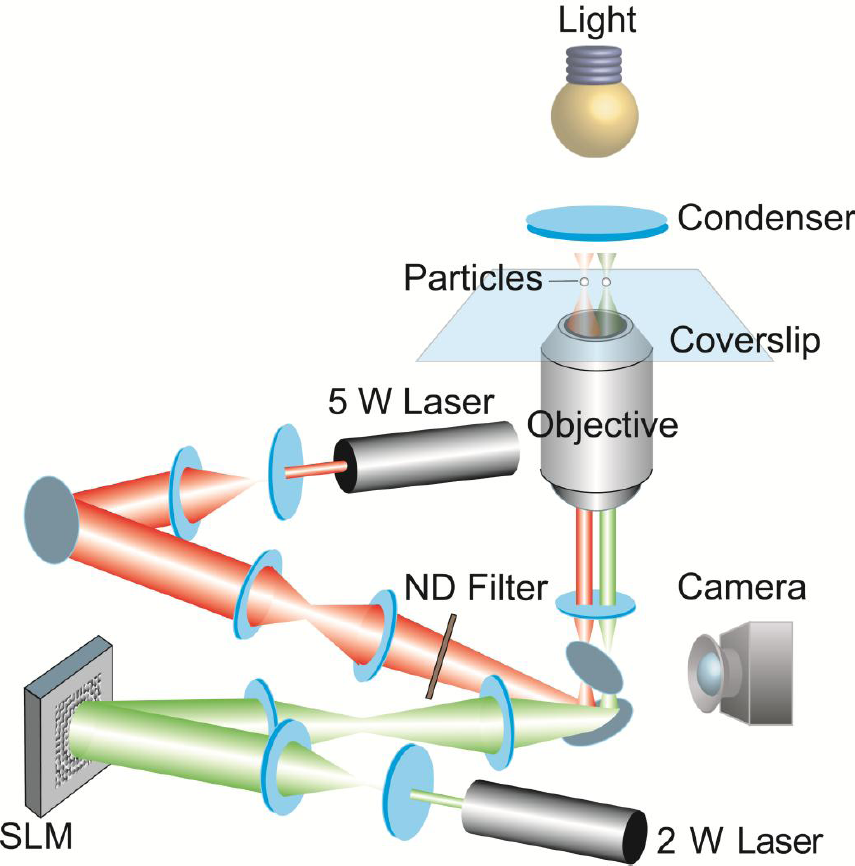
\includegraphics[width=0.9\textwidth]{Figures/chapter-intro/tweezers_configuration2.png}%
    \caption{\label{tweezers-configuration}}
  \end{subfigure}
  \begin{minipage}{0.35\textwidth}
  \begin{subfigure}{0.99\textwidth}
    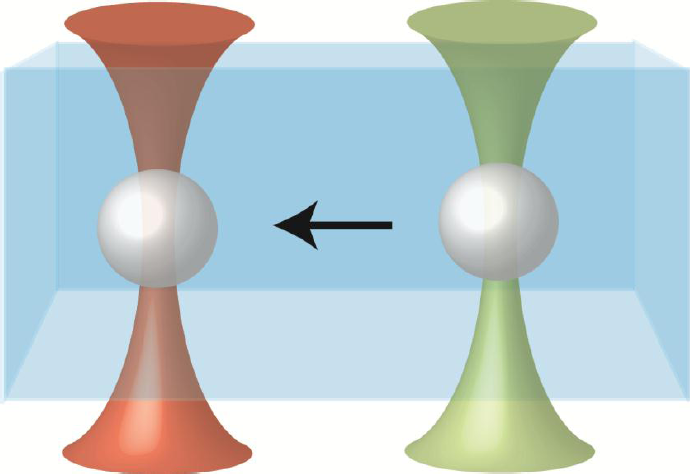
\includegraphics[width=0.9\textwidth]{Figures/chapter-intro/tweezers_particles.png}%
    \caption{\label{tweezers-particles}}
  \end{subfigure}%

  \begin{subfigure}{0.99\textwidth}
    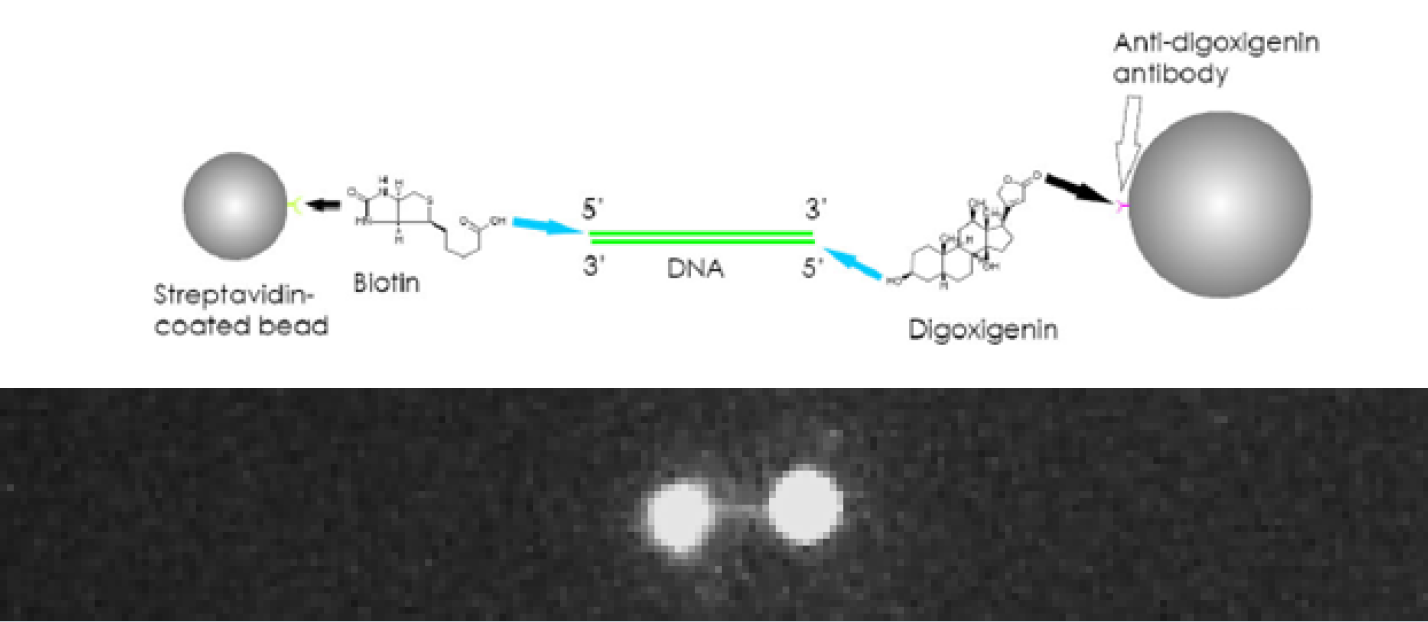
\includegraphics[width=0.9\textwidth,height=3cm]{Figures/chapter-intro/tweezers_linkage.png}%
    \caption{\label{tweezers-linkage}}
  \end{subfigure}
\end{minipage}

\caption[Optical Tweezers]{\protect\subref{tweezers-configuration} Current
optical tweezers configuration in our lab. \protect\subref{tweezers-particles}
Exertion of force moving the right trap. One of the bead (red-left) is fixed by
the most powerful trap. \protect\subref{tweezers-linkage} Linkage of the
 polymer stained with fluorescence particles (double stranded DNA) to the beads,
 and below, visualization of the fluorescence. Images by courtesy of group mate,
 Sandy Suei. }
\label{fig:optical_tweezers}
\end{figure}

%  Since the bending rigidity of the polymer is
% of the thermal energy order, the equilibrium length L_{eq} is determined by the
% transverse fluctuations of u.

Thanks to optical tweezers and Atomic Force Microscopy
(AFM)\citep{janshoff_force_2000} force-extension curves of many
biopolymers have been measured, e.g. DNA\citep{marko_stretching_1995},
polysaccharides\citep{marszalek_atomic_1999} and others. At low strain, the WLC
model captures well the system behavior, but at higher forces, a hookean
extension regime must be incorporated to account for enthalpic stretching
beyond the contour length.
Such a model is called \emph{extensible wormlike chain}
(EWLC)\citep{wang_stretching_1997}:

\begin{equation}\label{EWLC}
f(x)=\frac{\kbolt{}T}{\ell_p} \Big[ \frac{1}{4(1 - x/L_c + f(x)/K_0)^2}
-\frac{1}{4}+\frac{x}{L_c} + \frac{f(x)}{K_0}\Big]
\end{equation}


where $K_0$ is the elastic spring constant. Another model, the
\emph{clickable extensible wormlike chain} (CEWLC) incorporates extra
enthalpic components of the chain, for example taking into
account the conformational changes of sugar rings induced by high forces in polysaccharides\citep{haverkamp_model_2007}.


\begin{figure}[ht]
\begin{center}
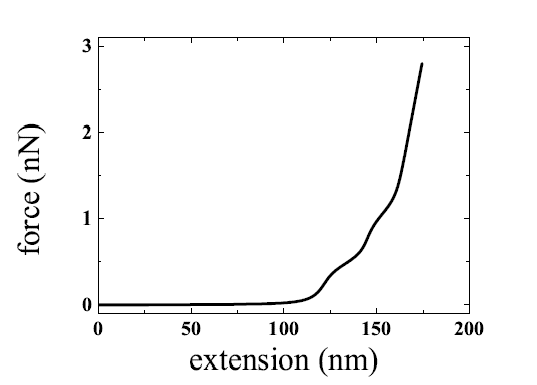
\includegraphics[width=0.7\textwidth,height=0.5\textwidth]{Figures/chapter-intro/forceextension_CEWLC.png}%

\caption[Force extension curve: CEWLC]{Force-extension curve of a CEWLC model
from Ref. \citep{schuster_hierarchical_2011}. It fits the experimental
force-extension curve of a single polysaccharide (pectin) chain \citep{haverkamp_model_2007} }
\label{fig:force_extension_CEWLC}
\end{center}
\end{figure}

\section{Networks of semiflexible chains:}
After the study of single chains, we have to study how all those chains interact
with themselves, with each other and with the media where they are.
The WLC is a model for ideal chains because the interaction between
monomers of the chain are ignored. This is not a problem in straight
(i.e. stiff) chains, but would be unrealistic in coiled chains, which are better
modeled with a self avoiding walk, where distant monomers cannot occupy the
same position, or with the inclusion of an excluded volume, that takes into
account the interaction between monomers, and the forbidden configurations.

The way the monomers of the chain interact with other monomers or with the
solvent has been studied for long time. The Flory interaction parameter $\chi$
which depends on temperature, and pressure of the system, is a way to
characterize it.
\begin{equation}\label{FloryInteraction}
\chi=\chi_{MS} - \frac{1}{2}(\chi_{MM} + \chi_{SS})
\end{equation}
where  $\chi_{MM}$ is related with monomer-monomer interactions. $\chi_{MS}$
with monomer-solvent, and $\chi_{SS}$ with solvent-solvent
interactions.

The relation between solvent, and monomers interaction can be classified using
$\chi$:
\begin{enumerate}
  \item Athermal. $\chi=0$. Solvent is very similar to other monomers.
  \item Good solvent. $\chi<1/2$. Monomers of the chain prefer to interact with
  the solvent than with other monomers.
  \item Poor solvent. $\chi>1/2$. Monomers prefer to be closer to other
  monomers. For example, hydrophobic materials in water solvent.
  \item Theta solvent. $\chi=1/2$. Occurs at a temperature $T=\Theta$, and
  corresponds to the exact cancellation between steric repulsion and van der
  Waals attraction between monomers. The excluded volume:
  \begin{equation}\label{excludedvolume}
  \upsilon=(1-2\chi)a^3
  \end{equation}
  where $a$ is the effective length between monomers, is zero in theta solvents,
  and chains behave as nearly ideal.\citep{gennes_scaling_1979}
\end{enumerate}

Also, the concentration of polymers has important effects on the system. The
overlap threshold parameter $c*$ acts as an order parameter to distinguish dilute
polymer solutions, where the coils are separate, and more concentrated solution
where the chains overlap. This threshold is not sharp, it is more properly
defined as a crossover between regions, but the scaling properties of $c*$ with
concentration are essential.
\begin{enumerate}
  \item Dilute. $c<c*$. Chains can be studied as an ideal gas, with almost no
  interaction between them.
  \item Dense. $c>c*$
  \item Semi-dilute. The chains do overlap but the polymer fraction
  $\phi=ca^3$ is still low $\phi*\ll\phi\ll1$. Since $\phi$ is small, the monomer-monomer interaction can
  be described very simply, such as with the excluded volume parameter
  $\upsilon$ in \ref{excludedvolume}. In the case of dense systems we would need more complex
  relations used in liquids/fluids systems.
\end{enumerate}


In dilute systems polymer chains flow through
the solvent, acting similar to a liquid state, in the other hand, dense system
are more like solids, but they are not completely frozen. The transition between
both regimes is called the gelation point. Th gelation is a connectivity
transition, where parts of the system becomes correlated by a path of
interconexion. In the gelation point, the chains stop to flow as a liquid. We
can think in an incipient gel, where a cluster of chains started to form (giant cluster), connecting the boundaries of the
material. This incipient gel will behave differently to a fully connected
network, where the giant cluster is connecting all the chains.

It is not easy to give a closed definition of
gels\citep{gennes_scaling_1979,rubinstein_polymer_2003}, I like to think about
it in these terms: it is the point in the phase space of parameters, where a significant correlation, between two points in the
spatial domain, appears over a length scale of the system size.
%Definition of gel, wikipedia UIAC.

\section{Bulk Rheology}
\subsection{Linear viscoelasticity}
Any elastic material can be studied as a linear spring, whereby the
extension (strain) $\gamma$ is proportional to the applied stress $\sigma$ (force/area) :
$\sigma=G'\gamma$ , where $G'$ is called the elastic modulus, and it is a
measure of sample's elasticity.

However, the material response to the force is not always that simple. Some
materials such as silk, rubber, and glass are subjected to a shear
stress and the corresponding Hooke's law deformation occurs, however it is
followed by an unexpected continuous deformation termed as ``creep''. Upon
removal of the shear stress, certain materials come back to the initial state,
while other are permanently deformed. The phenomena of a time dependant shear
response is called viscolelasticity. \citep{macosko_rheology:_1994}.

One way to study the deformation and flow of viscoelastic materials under
strain, is to externally apply a small amplitude
sinusoidal strain:
$\gamma(t)=\gamma_0\sin(\omega t)$. We can expect (not always, e.g. non-linear
regime) that the stress output of the material will be:
\begin{equation}\label{viscoelastic-response}
\sigma(t) = \sigma_0 \sin(\omega t + \delta)
\end{equation}
This stress output can be
analyzed by decomposition into two waves of frequency $\omega$, one in phase
with the strain, and the other $\pi/2$ out of phase:

\begin{equation}\label{viscoelastic-stress}
\sigma(t) = \sigma'(t) \sin(\omega t) + \sigma''(t)\cos(\omega t)
\end{equation}

where $ \tan \delta=\sigma''(t)/\sigma'(t)$. This allows the definition of two
moduli: $G'=\sigma'(t)/\gamma_0$ and $G''=\sigma''(t)/\gamma_0$ which are the
elastic (i.e. storage) modulus and viscous (i.e. loss) modulus respectively.

The stress can be expressed in terms of these two moduli:
\begin{equation}\label{viscoelastic-stress-G}
\sigma(t) = G'\gamma_0 \sin(\omega t) + G''\gamma_0\cos(\omega t) = G'\gamma(t)
 + \frac{G''}{w}\dot{\gamma}(t)
\end{equation}

$G''$ has a physical meaning, it is associated with the energy dissipation
per cycle of deformation, which provides and indication of viscous
loss \citep{macosko_rheology:_1994}. Note also that $\eta'=\frac{G''}{w}$
corresponds to the dynamic viscosity, used to characterize stress-response in pure liquids.

\subsection{Nonlinear behaviour: strain stiffening}
\label{intro-strainstiffening}
At small strain the stress-response is linear, but when the strain amplitude is
increased beyond a certain point, non-linear responses arise. In this situation,
the premise imposed in Eq.\ref{viscoelastic-response} that the stress response is linear does not
hold, however the qualitative study of $G'$ and $G''$ still provides information
about the nature of the non-linearities.
\citep{storm_nonlinear_2005,mackintosh_elasticity_1995,yao_nonlinear_2011,sheinman_nonlinear_2012,carrillo_nonlinear_2013}.

Fig. \ref{fig:strainstiffening-storm} shows that most of the biopolymer networks
share the same non-linear behaviour at high strains: strain-stiffening. In plain
words, the higher the strain is, the tougher the material becomes, or the more you pull,
the harder it is to pull more. The universal behavior in
biopolymers may have an evolutionary origin, due to the role of the strain-stiffening in biological functions such as cell motility
and mechano-transduction.

One way to study strain-stiffening experimentally is to use a \emph{large
amplitude oscillatory shear rheology} (LAOS) \citep{hyun_review_2011}. This
technique consists in pre-stress the network at a selected constant strain, and
then, study the frequency response applying other small amplitude sinusoidal strain, as in the
linear viscoelasticity situation.


 \begin{figure}[ht]
\begin{center}
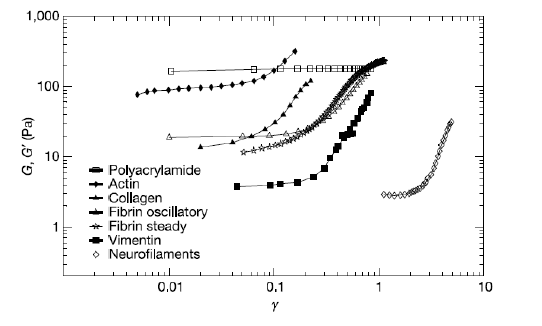
\includegraphics[width=0.7\textwidth,height=0.5\textwidth]{Figures/chapter-intro/strainstiffening_storm.png}%

\caption[Strain-stiffening in semiflexible
polymers]{ Elastic shear moduli versus
strain from Ref.\citep{storm_nonlinear_2005}. Strain-stiffening behavior in
different cross-linked biopolymer networks
\citep{carrillo_nonlinear_2013}.}
\label{fig:strainstiffening-storm}
\end{center}
\end{figure}


The research on strain-stiffening in biopolymers is really
active \citep{storm_nonlinear_2005, onck_alternative_2005,
head_distinct_2003,head_deformation_2003,wilhelm_elasticity_2003,huisman_three-dimensional_2007,yao_nonlinear_2011}.
Stiffening can result from the response of the chain between cross-links, from
alterations in the network structure, or from both.

 In a seminal paper,
\citet{storm_nonlinear_2005} showed that: for low to middle strains, under
the assumptions that networks are homogeneous, isotropic, and strain uniformly
(affine deformations), the strain-stiffening is primarily due to the
longitudinal stiffening of the single chains (i.e.
the non-linearity of the force response curve such as
Fig.\ref{fig:force_extension_CEWLC}).

 \begin{figure}[ht]
\begin{center}
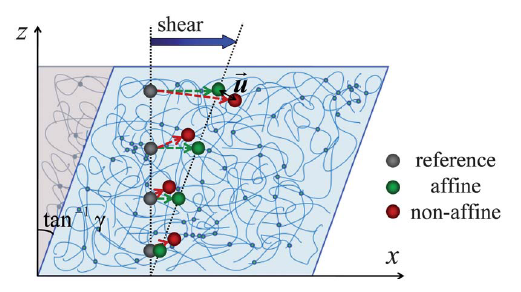
\includegraphics[width=0.6\textwidth]{Figures/chapter-intro/nonaffine.png}%

\caption[Affine and non-affine deformations]{ Difference between affine
and non-affine deformation of a network under shear. Figure adopted from
references \citep{wen_non-affine_2012,basu_nonaffine_2011}
}
\label{fig:nonaffine}
\end{center}
\end{figure}
The affine deformation assumption (Fig.\ref{fig:nonaffine}) is well-known in
network models for rubber elasticity, and allows for a relatively
simple description of the overall network response on the basis of the behavior
of a single filament. But, this assumption does not always hold.

The small-strain affine deformation assumption in two-dimensional
networks of straight filaments has
been studied in great detail by \citet{head_distinct_2003,head_mechanical_2005}
and \citet{wilhelm_elasticity_2003}, (Fig.\ref{fig:nonaffine-head}) who conclude
that network deformation is non-affine for compliant, low-density networks
and affine for stiff, high-density networks.
 \begin{figure}[ht]
\begin{center}
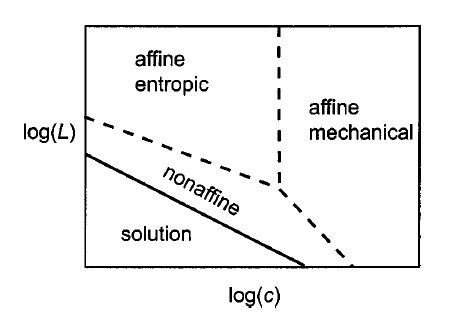
\includegraphics[width=0.6\textwidth]{Figures/chapter-intro/nonaffine-head.png}%

\caption[Affine and non-affine phases]{ Figure from
\citet{head_mechanical_2005}. Diagram showing the various elastic regimes in
terms of molecular weight (L) and concentration (c). The solid line represents
the rigidity percolation transition, where rigidity first appears at
macroscopic level}
\label{fig:nonaffine-head}
\end{center}
\end{figure} 

 Also, \citet{chandran_affine_2006}
showed that non-affinity governs individual fibril kinematics when the load
transfer is from fibril to fibril, with no matrix of fibrils involved.

% motivation link
\section{Motivation}%
\label{sec:motivation-intro}
Non-affinity and network architecture or connectivity are closely related, which
is the \textbf{main motivation} behind this work to stablish analytical methods to study images
from where gather the geometry of networks.

The well-established and trusted method to gather structural information of the size of the network
is scattering, particularly small-angle x-ray scattering (SAXS). Information such as porous
size and persistence length are at range of these techniques. However, because its
averaging nature, it is impossible to gather more detailed information about the specific geometry
and connectivity of the network.

So we will rely on gathering structural information directly from images taken from a range microscopy techniques depending on the size of the biopolymer under study.
One of the concerns of this approach, shared specially among the scattering community is: can we trust the images, does it provide a true representation of the material taken into account that the sample has been modified for the requirements of microscopy preparation? We will answer this, providing a way to compare SAXS data with images, setting the scale at which both techniques give similar result, providing a size range where image features can be trusted.

But before, and in order to study network geometry reliably, we need to provide an image analysis tool-set with algorithms that can be applied to volumetric data, such as tomography and stack of images.
We will extend to 3D, and in a high-performance computing language, state-of-the-art wavelet analysis algorithms, that will aid in our task of gathering the network architecture from images.
We then extract in-silico networks from real 3D images.
These in-silico networks with full details, can be used by theoreticians as starting points for non-affinity modeling, instead of the currently most-used random mikado methods which only generates homogeneous and isotropic networks.
We finish providing a method to reconstruct these networks fully in-silico, just with statistical
distributions gathered from the networks extracted from real images. This allow exploration and speculation of optimal network architectures for different processes completely in-silico, but rooted on networks found in nature.


% Chapter Template

\chapter{Spatial Graph Extraction: Analysis of microscopy images to obtain network architecture} % Main
% chapter title

\label{Chapter-Image} % Change X to a consecutive number; for referencing this
% chapter elsewhere, use \ref{ChapterX}

\lhead{Chapter 4. \emph{Spatial Graph Extraction}}

\section{Motivation}%
\label{sec:motivation-image}

The goal of this chapter this chapter is two folds: report denoising and segmentation methods applied to 3D images of biopolymer networks, and from a binary image, obtain a spatial graph representation of the material, which encodes the connectivity and geometry of the network.
The spatial graph abstraction can be used to characterize the network studying statistical distributions of different properties of the graph, but also as a direct way to encode the architecture in a format usable by computational models of network behaviour under strain.

\section{Introduction}%
\label{sec:introduction}

The geometry or architecture of a biopolymer network impacts its mechanical
properties and biological functions.
The goal of this chapter is to explain the algorithms and software used to
obtain an abstract representation, a \gls{Spatial Graph}, of this architecture from volumetric images taken from any microscopy technique.

A \gls{Spatial Graph} (see \autoref{fig:spatial_graph_intro_1}), is a graph containing geometrical information about the image from which it is extracted. It is defined by two sets:
\begin{itemize}[topsep=0pt]
  \item A set of nodes or vertices (i.e. end-points or junctions), characterizing the spatial position of chain junctions.
  \item A set of edges (i.e. links), connecting pairs of those nodes. The geometric information is contained in a set of ordered edge points, reflecting the path of the connection.
\end{itemize}

The graph connectivity is described by an adjacency list \autoref{fig:spatial_graph_intro_2}, with extra labels representing the position of nodes, and the set of edge points.
\begin{figure}[!htb]
  \centering
  \begin{subfigure}{0.5\textwidth}
    \centering
    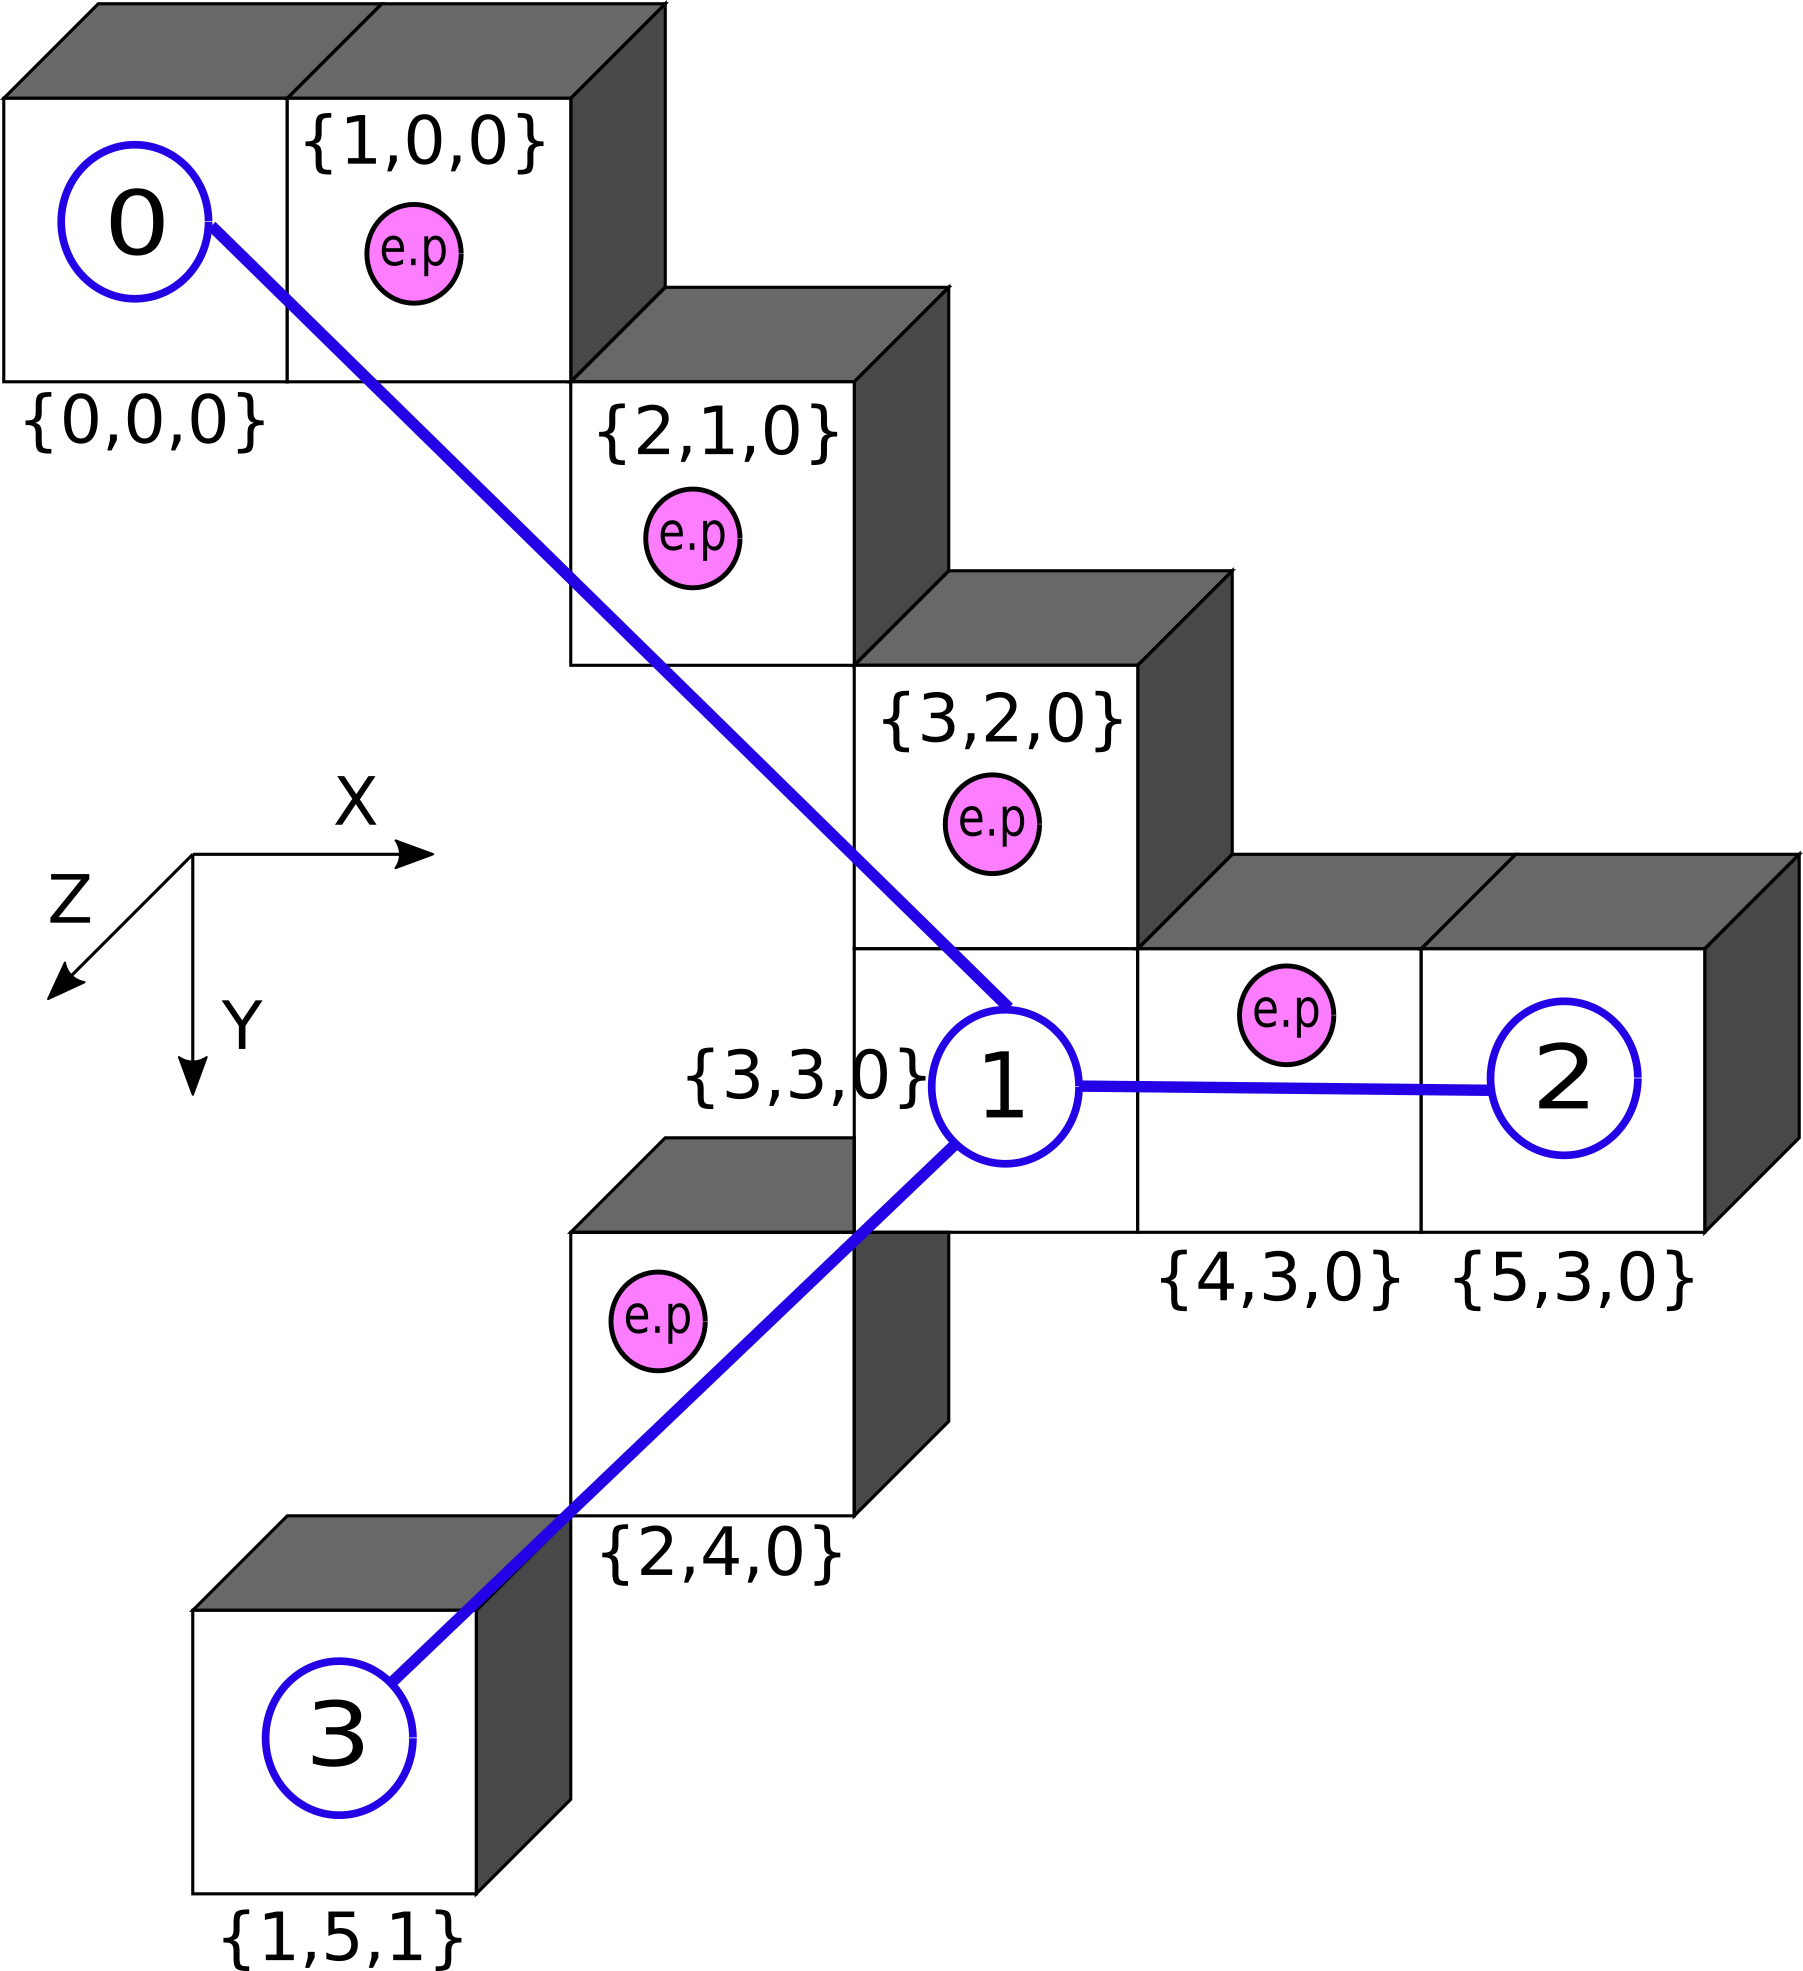
\includegraphics[width=0.6\textwidth]{Figures/chapter-image/spatial_graph_intro1.png}%
  \caption{\gls{Spatial Graph} extracted from a set of voxels. Numbers in circles represent each node id. In brackets, the index position of each voxel.}
    \label{fig:spatial_graph_intro_1}
  \end{subfigure}%
  \begin{subfigure}{0.5\textwidth}
    \centering
    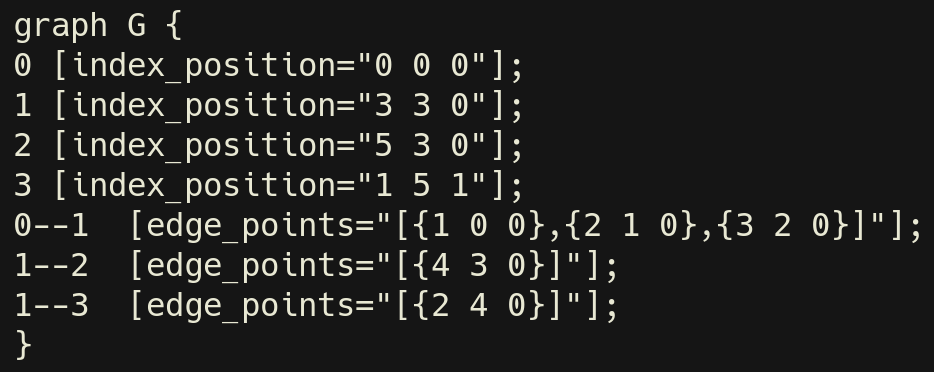
\includegraphics[width=0.9\textwidth]{Figures/chapter-image/spatial_graph_intro2.png}%
    \caption{Adjacency list representing the graph with labels containing the index position of nodes and edges points.}
    \label{fig:spatial_graph_intro_2}
  \end{subfigure}%
  \caption{Visualization of a \gls{Spatial Graph} (\ref{fig:spatial_graph_intro_1}) and the corresponding adjacency list (\ref{fig:spatial_graph_intro_2}).
    The graph is represented in blue, formed by nodes (voxels with id) and edges connecting them.
  The voxel positions (in brackets in \ref{fig:spatial_graph_intro_1}) of nodes and edge points are stored as labels in the adjacency list.}
  \label{fig:spatial_graph_intro}
\end{figure}

The following representation fully contains all the information needed to describe a network structure, as described elsewhere \cite{palmer_constitutive_2008}:
\begin{enumerate}[topsep=0pt]
  \item Distribution of the distance between nodes, i.e. end-to-end distances.
  \item Distribution of the fully extended length of edges, i.e. contour lengths.
  \item Network connectivity, i.e. degree of nodes: representing the number of other nodes connected to it.
  \item Orientation distribution. i.e. angles and direction cosines of angles between adjacent edges.
\end{enumerate}

Firstly, to accomplish a reliable extraction of the spatial graph from volumetric images, the image processing analysis used to segment the biopolymer from images will be introduced, this includes the pre-processing and denoising steps in \autoref{sec:denoising} and the binarization in \autoref{sec:segmentation}.

Secondly, the thinning or skeletonization
algorithm developed for creating a thin (one-pixel wide) image representation of the network in \autoref{sec:skeletonization} will be presented.

Thirdly, from the resulting thin image, the abstract representation in form of the described \gls{Spatial Graph} will be discussed in \autoref{sec:spatial_graph_extraction}.

Once extracted, any \gls{graph} property can be computed from our extracted spatial graph using the tool-set of complex networks,
from degree distribution to clustering coefficient. In addition also the spatial information allows us to compute geometric quantities, such as distance between nodes or angle between adjacent edges.

Finally, statistical distributions will be computed from our extracted graphs: degrees, end-to-end distances, contour lengths and direction cosines, that capture, in an analytical form, the network architecture (\autoref{sec:statistical_distributions_of_graph_properties}.

\textbf{Outline:}
\begin{enumerate}
  \item \hyperref[sec:denoising]{Denoising}

  \item \hyperref[sec:segmentation]{Segmentation}

    \begin{itemize}
      \item \hyperref[sub:binarization]{Binarization}
      \item \hyperref[sub:hole_filling]{Hole Filling}
    \end{itemize}

  \item \hyperref[sec:skeletonization]{Thinning / Skeletonization}

    \begin{itemize}
      \item \hyperref[sub:critical_kernels_framework]{Critical Kernels Framework}
    \end{itemize}

  \item \hyperref[sec:spatial_graph_extraction]{Spatial Graph Extraction}
\end{enumerate}

% Second, we will explain the two
% methods that we have tested, FIRE and Avizo. At the same time, using confocal
% images of actin networks obtained from our lab,  we will extract statistical
% distributions of some properties of the network using both algorithms. Finally,
% we will compare the results from both algorithms, and comment about future
% directions and improvements.

\subsection{Notation}%
\label{sub:notation}

 The \textbf{pixel}, \textbf{pixel position}, or \textbf{pixel index} is defined as:
 $\vect{p}\equiv(x,y,z)\, \epsilon \,V$, where
 $x\eps{}[0,X - 1]$, $y\eps{}[0,Y - 1]$, $z\eps{}[0,Z - 1]$ are the integer coordinates and
 $V\subset \mathbb{I}^3$ is the volume of the stack of images $V=\{X\times
 Y\times Z\}$.
 With $Z$ the number of images in the stack, and $X,Y$ the size of the $2D$ images.

 \textbf{Pixel value} or \textbf{pixel intensity} refer to the value of the pixel in the corresponding
 image.
 The value could be an integer, a boolean, or a real number, depending on the type of image:
 gray-scale, binarized or a distance map.
 The original \textbf{gray-scale image} $I$ is defined as:
 $I(\vect{p}):V \longrightarrow G$ where
 $G$ is a set of integers representing the gray-scale.
 $G=\{0,1,\ldots,G_M\}\subset\mathbb{I}$ where $0$ represents black, $G_M$
pure white, and the others correspond to different gray-scale values. $G_M=255$
in $8$ bits images, and $G_M=2^{16} - 1 = 65535$ in higher quality images of $16$ bits.

The \textbf{binarized image} B is defined as the map:
$$f_B: I \longrightarrow B_T \,\,|$$ 
\begin{equation}
 B_T(\vect{p})=
   \begin{cases} 
     1               & \mbox{if } I(\vect{p}) > T   \\
     0               & \mbox{if } I(\vect{p}) < T
   \end{cases}
   \label{eq:bin}
\end{equation}
Where $T\eps{}G$ is the threshold value of the binarization. The threshold can also be expressed as
a normalized intensity value $T_P \eps{}[0,1]\subset \mathbb{R}$. If
$I_{max}\eps{}G$ is the max value of $I$, then the threshold  is
$T=round(T_P \cdot I_{max})$  where the round function converts a real number
into the nearest integer. The binary threshold can also be characterized with a percentage of the
brightest gray-scale value involving
cumulative histograms of $I$.

\section{Denoising}%
\label{sec:denoising}

Pre-processing the image to remove spurious noise is fundamental to obtain a good segmentation of our network in the next step.

% Add/Show wavelet denoising, and TotalVariation (proxTV)
The wavelet tools developed in ~\autoref{Chapter-Wavelets} were used to perform a phase analysis \cite{held_steerable_2010} in the image. This will equalize local brightness differences, and homogenize intensity values of foreground objects. Then, an anisotropic denoising is performed, which avoids blurring information in edges of objects.

Total variation regularization \cite{barbero_fast_2011, barbero_modular_2014} methods were applied to our 3D images, showing effective denoising and maintaining sharp transitions between edges of objects and background.

% Figure with results, one for each process.
\begin{figure}[!htb]
  \centering
  \begin{subfigure}{0.33\textwidth}
    \centering
    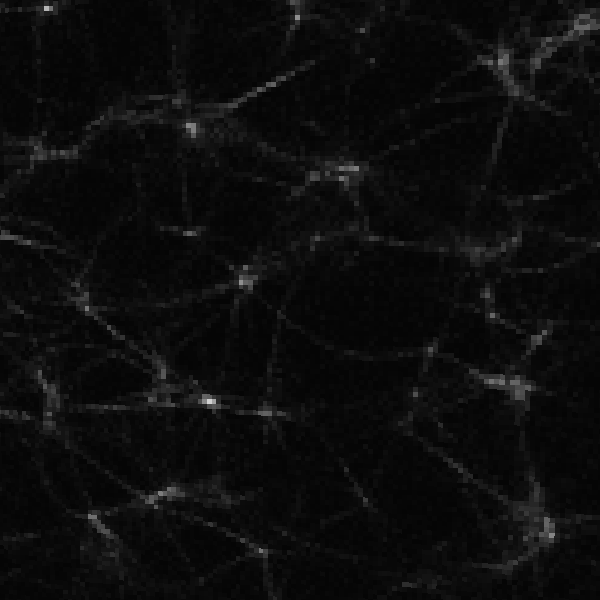
\includegraphics[width=0.95\textwidth]{Figures/chapter-image/denoise_actin1_original.png}%
    \caption{Original}
    \label{subfig:denoise_original}
  \end{subfigure}%
  \begin{subfigure}{0.33\textwidth}
    \centering
    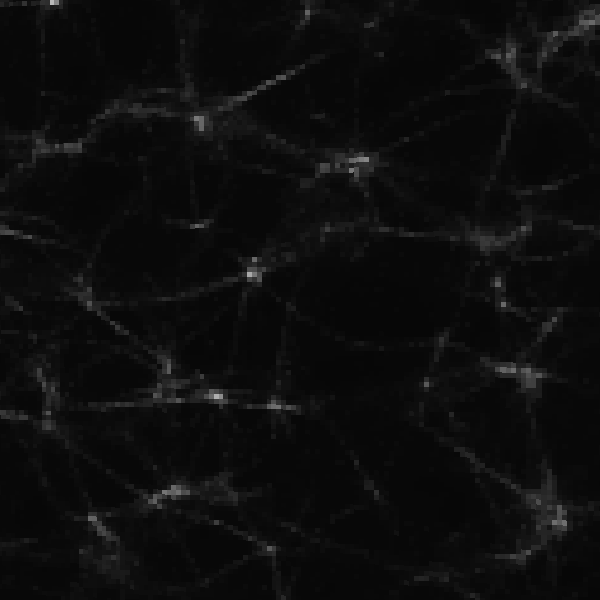
\includegraphics[width=0.95\textwidth]{Figures/chapter-image/denoise_actin1_tv1.png}%
    \caption{Total Variation $\lambda = 1$}
    \label{subfig:denoise_tv}
  \end{subfigure}%
  \begin{subfigure}{0.33\textwidth}
    \centering
    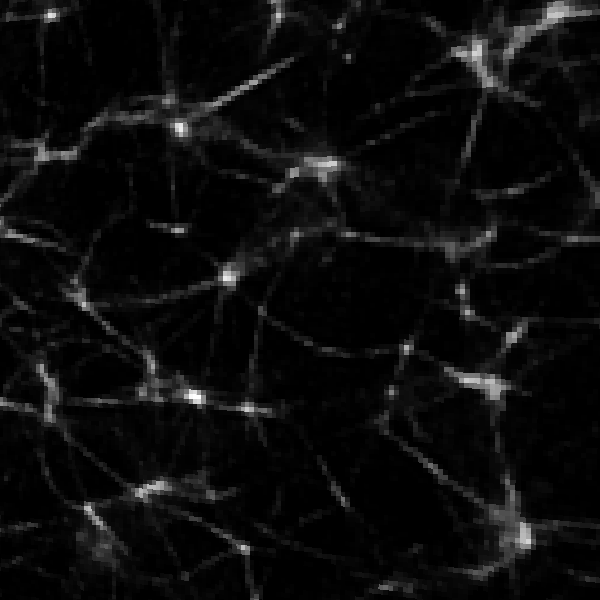
\includegraphics[width=0.95\textwidth]{Figures/chapter-image/denoise_actin1_wavelet.png}%
    \caption{Wavelet based}
    \label{subfig:denoise_wavelet}
  \end{subfigure}
  \caption{Pre-processing the image (actin): denoising with wavelets and total variation methods.}
  \label{fig:denoise}
\end{figure}


\section{Segmentation}
\label{sec:segmentation}

Segmentation refers to the extraction of the objects of interest from an image, discarding the rest of information. When the image is composed by many different objects, with different shapes and pixel
intensities, complex approaches must be taken to reliably extract the objects of interest.
For example in biology the segmentation might want to extract only cells of certain type from an
image with many other actors.

In our case, our images are only composed by biopolymers, so our segmentation is easier, it reduces
to a binarization task: separate background and noise from the biopolymer objects.

Easier doesn't mean easy though, grouping all the information into two clusters is inherently hard.
The goal is to find an intensity value that acts as a threshold for the two groups.
If the intensity along the image is not bright-normalized, it might happen that objects with absolute lower intensity are lost.
This is the reason why a local approach using a region growing algorithm is preferred, where first seeds in the middle of our object of interest are selected, and then, the algorithm will grow those seeds to fill the whole region of interest based on intensity differences between neighbor pixels and the seeds.

Any binarization filter is seriously affected by noise present in the images. That is why the pre-processing and denoising step is fundamental to get a reliable result from this process.

\subsection{Binarization}
\label{sub:binarization}
The gray levels of pixels belonging to an object are substantially
different from the gray levels of the background. Thresholding is a way to
separate objects from the background.

\citet{sezgin_survey_2004} is a good review about the subject. The output of the
thresholding process is a binary image, whose one state will indicate the
foreground objects, while the complementary state will correspond to the
background.

\begin{figure}[!htb]
\begin{subfigure}{0.5\textwidth}
  \centering
  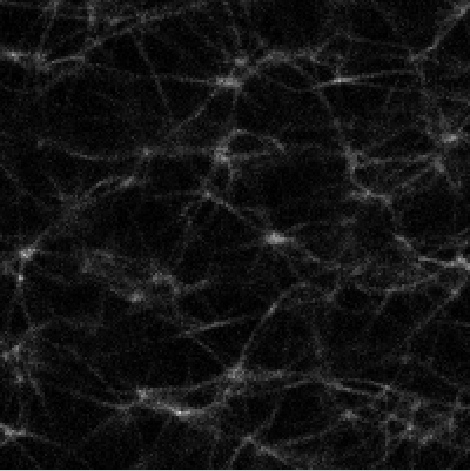
\includegraphics[width=0.9\textwidth]{Figures/chapter-image/binary/fig_bin_original.png}%
  \caption{Input Image - Original}
  \label{binoriginal}
\end{subfigure}%
\begin{minipage}{0.5\textwidth}
  \centering
  \begin{subfigure}{0.5\textwidth}
    \centering
    
\includegraphics[width=0.9\textwidth]{Figures/chapter-image/binary/fig_bin_01.png}%
    \caption{$T_P$=0.01}
    \label{bin001}
  \end{subfigure}%
  \begin{subfigure}{0.5\textwidth}
    \centering
    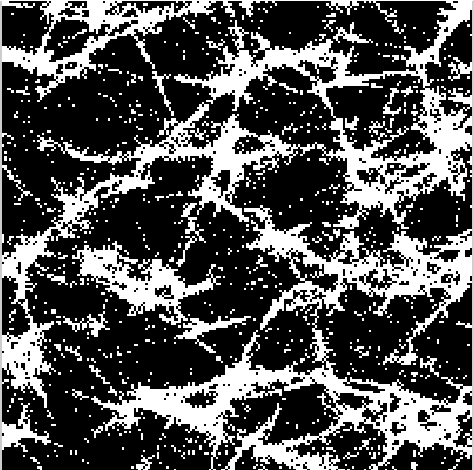
\includegraphics[width=0.9\textwidth]{Figures/chapter-image/binary/fig_bin_08.png}
    \caption{$T_P$=0.08}
    \label{bin008}
  \end{subfigure}

  \begin{subfigure}{0.5\textwidth}
    \centering
    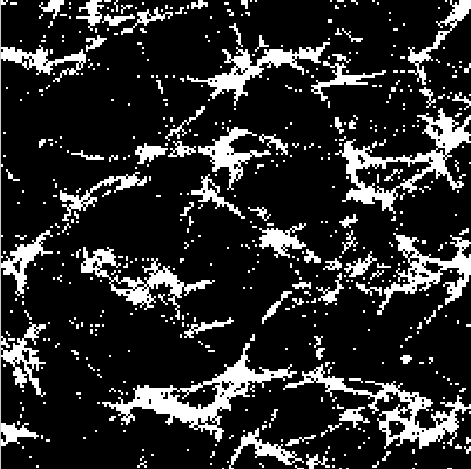
\includegraphics[width=0.9\textwidth]{Figures/chapter-image/binary/fig_bin_01176Otsu.png}%
    \caption{$T_P$=0.1176}
    \label{binotsu}
  \end{subfigure}%
  \begin{subfigure}{0.5\textwidth}
    \centering
    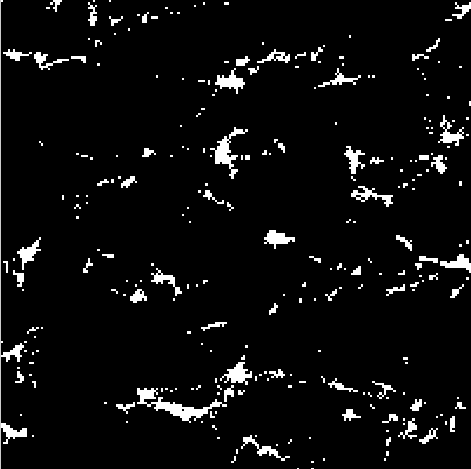
\includegraphics[width=0.9\textwidth]{Figures/chapter-image/binary/fig_bin_20.png}%
    \label{bin020}
    \caption{$T_P$=0.20}
  \end{subfigure}%
\end{minipage}

\caption[Different threshold values on networks]{Different threshold values applied to a confocal image of an actin network.
$T_P$ is a normalized threshold value, if $G_{max}$ is the brightest pixel, then
$T=T_P\cdot P_{max}$. According to eq \ref{eq:bin}, any pixel which value is greater than T transforms to $1$
(white) after the binary filter.
At low values of threshold (case \subref{bin001}), networks are blurred, but
at high values (case \subref{bin020}), some connectivity information is lost.
The case \subref{binotsu} corresponds to the threshold calculated by Otsu's
method.}
\label{fig:binary}
\end{figure}

A significant body of work already exists on thresholding. One of the most famous binary
filters is Otsu's method, which minimizes the weighted sum of within-class variances of the
foreground and background pixels to establish an optimum threshold
\citep{sezgin_survey_2004}. This method belongs to the clustering-based methods
of thresholding. Further classification of thresholding is based on:
\begin{itemize}
  \item \textbf{Histogram shape.} Peaks, valleys and curvatures of the smoothed
  gray-level histogram are analyzed. \emph{Peak-and-valley}.
  \item \textbf{Clustering.} The gray levels are clustered in two parts, one
  corresponding to the background and the other to the foreground. This method
  analyses separately each cluster. \emph{Otsu, Minimum error, fuzzy}.
  \item \textbf{Entropy.} Exploits the entropy of the distribution of the gray
  levels in the image. Maximization of entropy is indicative of high information transfer.
  Low cross-entropy between input gray level and output binary means
  preservation of information. \citet{pal_automatic_1983}
  were the first to use Shannon entropy in image analysis.
 \citep{pal_image_1988}
  \item \textbf{Object attribute.} Select the threshold based on some attribute
  quality between the original and binarized image. \emph{Edge matching, connectivity,
  shape compactness}.
  \item \textbf{Spatial methods}. This class not only uses the gray
  distribution, also studies the dependency of pixels in a neighborhood, for example, correlation
functions or co-occurrence probabilities.
  \item \textbf{Local adaptive methods.} A threshold is calculated at each
  pixel, which depend on some local statistics, like \emph{variance}.
  \item \textbf{Region growing.} The binarization starts from seed pixels placed in the interior
    of objects wanted to be segmented. These algorithms study the neighborhood of these seeds and under some criteria, for example intensity difference, it adds the neighbor pixel to the foreground region. The process is repeated until no new pixel is added.
\end{itemize}

For our purposes, the binarization threshold will have an impact in obtaining the
network. If the threshold is too high, long fibers will break in short,
unconnected pieces. If the threshold is too low, fibers that are clearly
separated, will become blurred together.

In Fig.\ref{fig:binary}
the geometry of a small area of an actin network is compared after
applying different binary thresholds. The stack of images of
networks used here was obtained in our group by Dr. Allan
Raudsepp using confocal microscopy on actin.

\subsubsection{Region Growing Segmentation}%
\label{subsub:region_growing_segmentation}

The risk of region growing algorithms is that a seed will be planted outside our foreground objects. However, I have found planting the seeds with a normalized threshold $T_p$ I don't have to fine tune the lower threshold too much. The results are quite resilient against small changes of these parameters, where a pure thresholding approach will suffer a lot of variation and be prone to noise artifacts.

Using \href{https://itk.org/Doxygen/html/classitk_1_1ConnectedThresholdImageFilter.html}{itk::ConnectedThresholdImageFilter} with the script:
\href{https://github.com/phcerdan/ITKfilters/blob/master/scripts-cpp/regionGrowingSegmentation.cxx}{regionGrowingSegmentation.cxx}

\noindent\textbf{Parameters:}

\begin{itemize}[topsep=0pt]
  \item \textbf{Lower threshold} and \textbf{upper threshold: } The region won't grow into pixels outside these limits. Combined with a conservative $T_p$ for initial seeds the results do not change with small variation of these parameters.
  \item \textbf{Normalized Threshold $T_p$ for initial seeds: } Create initial seeds based on a normalized binary threshold. Taking a conservative low value, the region will grow from these seeds to fill the object.
\end{itemize}

\subsection{Hole Filling}%
\label{sub:hole_filling}

Due to noise, tiny holes might still be created in the binarization process. These holes (areas of OFF pixels surrounded by ON pixels) have an important effect in the following skeletonization step because they change the topology of the object and the network to be extracted. To solve it, an aggressive fill of these small holes with an iterative hole filling algorithm is realized.


Using \href{https://itk.org/Doxygen/html/classitk_1_1VotingBinaryIterativeHoleFillingImageFilter.html}{itk::VotingBinaryIterativeHoleFillingImageFilter} with the script:
\href{https://github.com/phcerdan/ITKfilters/blob/master/scripts-python/binary_denoise_3d_fillholes_iterative.py}{binary denoise 3D fillholes}

\noindent\textbf{Parameters:}

\begin{itemize}[topsep=0pt]
  \item \textbf{Majority: } Number of ON pixels in the neighborhood of an OFF pixel, to switch it into ON. By default, majority = 1, this means that an off pixel will be turned on if in the neighborhood (set by radius) there are at least 50\% + 1 pixels ON. If $\text{radius} = \{1,1,1\}$ neighborhood size will be $3\times3 = 9$ pixels. If 5 pixels around an OFF pixel are ON, then it will be switched.
  \item \textbf{Neighbor Radius: } Number of neighbors to check. $R = 1$ in 3D is a $3\times3\times3$ neighborhood.
  \item \textbf{Iterations: } Number of iterations before stopping, the algorithm also stop if no changes are generated after last iteration.
\end{itemize}

A high value of majority and a small neighborhood is selected to only fills small holes, but let bigger empty spaces unaffected. \newline
For 3D images, a value of:\newline
Majority = 3, Radius = 1, Iterations = $\infty$ works well for our purpose of removing just small holes.


\section{Skeletonization}%
\label{sec:skeletonization}

The skeleton of an object is a representation of the object, which contain both,
shape features and topological structures of the original object. It is widely
used in computer graphics, character recognition, and analysis of biomedical
images.\citep{bai_skeleton_2007,golland_fixed_2000,ge_generation_1996}. The
skeletonization is very sensitive to noise and boundary deformations, which generates redundant skeleton branches that disturb the
topology of the skeleton graph (Fig.\ref{fig:skeleton-fixedtopo}(b)). This being the reason why the mentioned pre-processing steps of the image are important for a reliable skeletonization.

What are then the desirable properties of a skeletonization process?
\begin{enumerate*}[label=\textbf{\alph*)}]
  \item Preserves the topology of the original object, i.e. it has the same tails
  and holes.
\item Generates a minimal or thin skeleton, i.e. the width of the skeleton is one point, only containing points which removal would alter the topology.
  \item The skeleton is centered in the object.
  \item Stable under small deformation of the boundaries (noise) of the object, not generating spurious branches.
\end{enumerate*}

There is no single skeletonization algorithm in the literature that fully complies with all these desirable properties, the more difficult being the robustness against rough and noisy boundaries.

\begin{figure}[!htb]
  \centering
  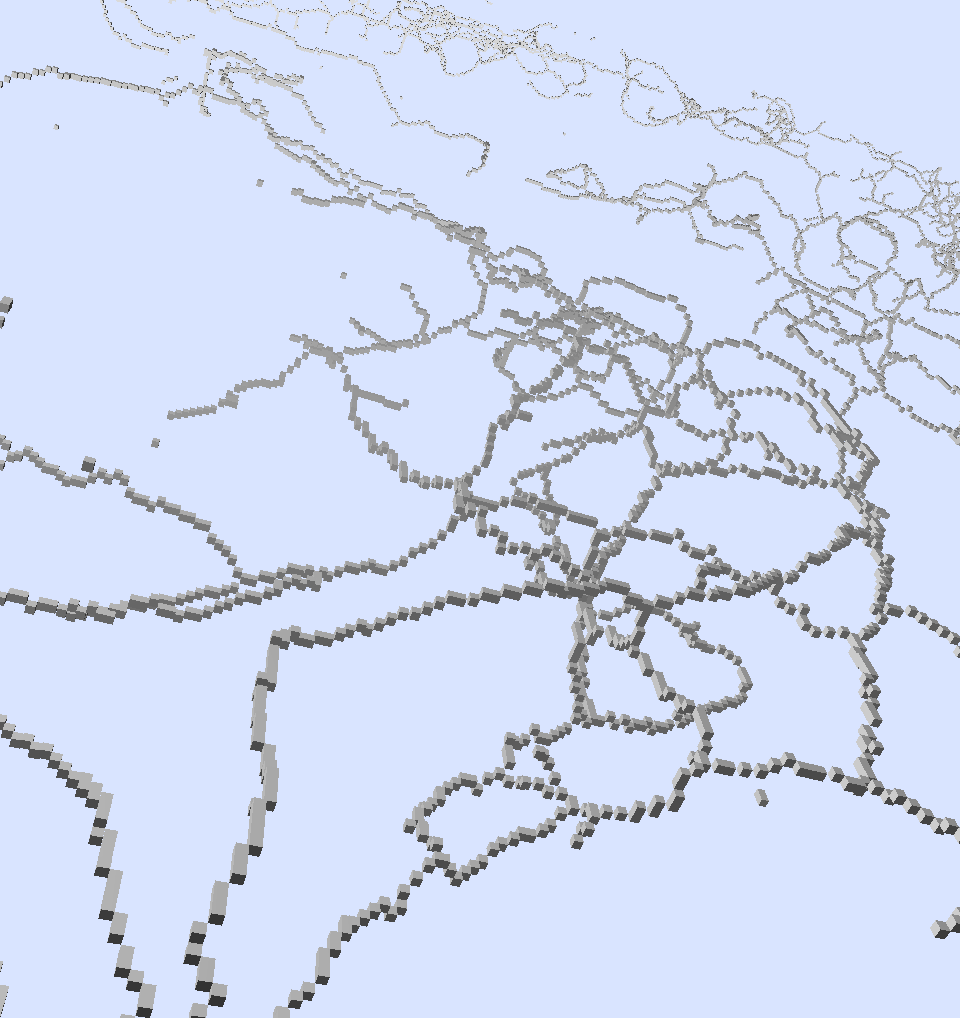
\includegraphics[width=0.8\textwidth]{Figures/chapter-image/skeleton_3D_viewer.png}%
  \caption{Thin image of a pectin network after skeletonization performed with the critical kernels framework (see \autoref{sub:Pectin}) and visualized with a 3D Viewer. The skeleton keeps the topology of the original object, is thin, centered, and robust against rough and noisy boundaries.}
  \label{fig:thin_3Dviewer}
\end{figure}

The most important skeletonization algorithms can broadly be classified by:

\begin{enumerate}
  \item \label{itm:voronoi} Based on Voronoi diagrams \citep{ogniewicz_hierarchic_1995}.
    These methods search the locus of centers of the maximal disks
    contained in the contour of the object. The skeleton can be
    extracted with accurate position and topology, but the time
    of computation is usually prohibitive, and the complicated skeleton needs to be
    pruned due to spurious branches.
  \item \label{itm:ridges} Based on detecting ridges
    in the distance map from the boundary points. The
    position of the skeleton is centered, but does not guarantee to preserve
    the same topology than the original object
    \citep{ge_generation_1996}.
    % The two methods analyzed from literature are based on
    % this kind of skeletonization.
  \item \label{itm:simple} Based on iteratively peeling off points from the boundary of the object \cite{palagyi_sequential_2001,brimkov_topology_2012}. The only points of the object that are deletable are simple points (a point is simple if its deletion preserves
    the object topology). The generated skeleton preserves the topology of the object, however is not guaranteed to be centered. The simple points can be removed sequentially or in parallel.
    The order in which these points are selected affects if the skeleton is thin and/or centered. However the skeleton is not stable except for small objects, usually generating many spurious branches.
  \item \label{itm:critical} Based on the critical kernels framework \cite{couprie_asymmetric_2016}. The generated skeleton keeps the same topology than the original object, is thin, and the skeleton is much more stable compared to the removal of just simple points, generating less spurious branches. The original implementation \cite{couprie_asymmetric_2016} does not guarantee centered skeletons, but it can be enforced with the help of a distance map.
\end{enumerate}

\subsection{Distance maps}%
\label{sub:distance_maps}

The distance map calculates the distance from a
white pixel to the nearest black pixel. Every white pixel in the binary image
has now a real value calculated using any selected distance function (euclidean,
quasi-euclidean,\ldots ). Distance maps can be calculated from a binary image, or from
any image with shapes that are labeled differently.
Fig.\ref{fig:distancemap} has some distance maps of actin networks.
Fig.\ref{fig:fire_LMPS} shows the values of a distance map which have
been simplified from real to integer numbers for clarity.

\begin{figure}[H]
\begin{minipage}{0.5\textwidth}
  \centering
  \center{\textbf{Binarization}}\\
  % \begin{minipage}{0.5\textwidth}
  \begin{subfigure}{0.5\textwidth}
    \centering
    
\includegraphics[width=0.9\textwidth]{Figures/chapter-image/binary/fig_bin_01.png}
    \caption{$T_P$=0.01}
  \end{subfigure}%
  \begin{subfigure}{0.5\textwidth}
    \centering
    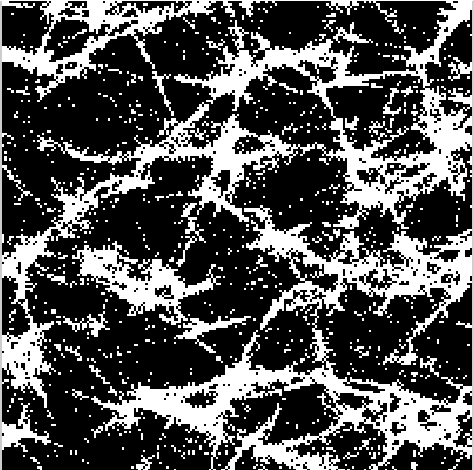
\includegraphics[width=0.9\textwidth]{Figures/chapter-image/binary/fig_bin_08.png}
    \caption{$T_P$=0.08}
  \end{subfigure}

  \begin{subfigure}{0.5\textwidth}
    \centering
    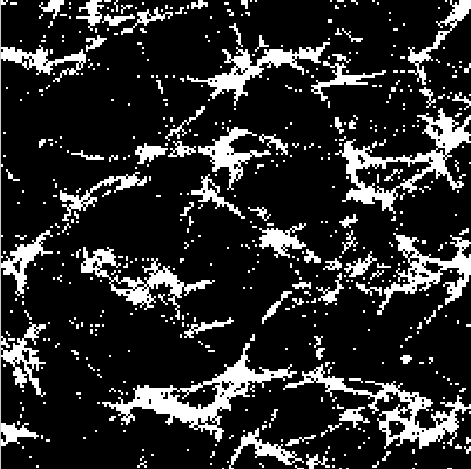
\includegraphics[width=0.9\textwidth]{Figures/chapter-image/binary/fig_bin_01176Otsu.png}
    \caption{$T_P$=0.1176}
  \end{subfigure}%
  % \hspace{1pt}
  \begin{subfigure}{0.5\textwidth}
    \centering
    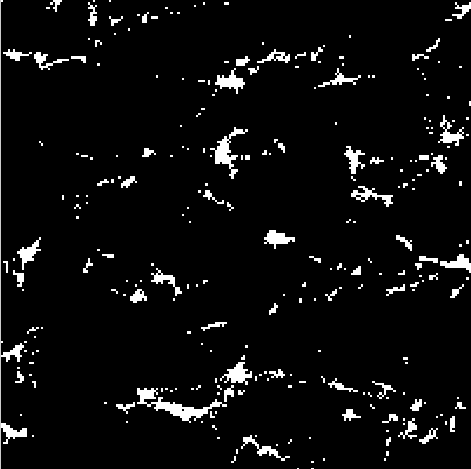
\includegraphics[width=0.9\textwidth]{Figures/chapter-image/binary/fig_bin_20.png}
    \caption{$T_P$=0.20}
  \end{subfigure}%
\end{minipage}
\begin{minipage}{0.5\textwidth}
  \centering
  \center{\textbf{Distance map}}\\
  \begin{subfigure}{0.5\textwidth}
    \centering
    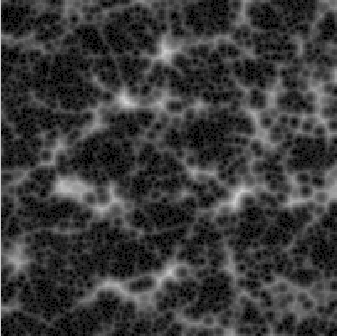
\includegraphics[width=0.9\textwidth]{Figures/chapter-image/distance/fig_dist_01.png}
    \caption{$T_P$=0.01}
  \end{subfigure}%
  \begin{subfigure}{0.5\textwidth}
    \centering
    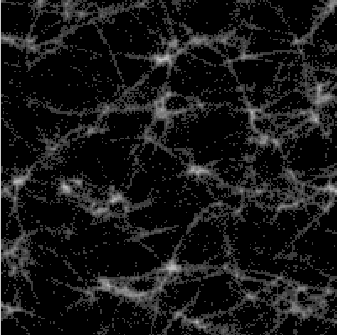
\includegraphics[width=0.9\textwidth]{Figures/chapter-image/distance/fig_dist_08.png}
    \caption{$T_P$=0.08}
  \end{subfigure}

  \begin{subfigure}{0.5\textwidth}
    \centering
    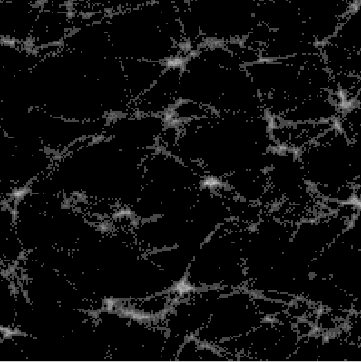
\includegraphics[width=0.9\textwidth]{Figures/chapter-image/distance/fig_dist_01176Otsu.png}
    \caption{$T_P$=0.1176}
    \label{distotsu}
  \end{subfigure}%
  \begin{subfigure}{0.5\textwidth}
    \centering
    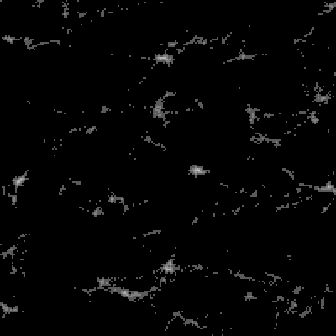
\includegraphics[width=0.9\textwidth]{Figures/chapter-image/distance/fig_dist_20.png}
    \caption{$T_P$=0.20}
    \label{dist014}
  \end{subfigure}
\end{minipage}
\caption[Distance map - Actin]{Example of distance maps calculated from binarized images
with different normalized thresholds $T_P$. Images (A) to (D) show binarization images with increasing threshold and (E)-(H) show the associated distance maps. In (A) the threshold is too low, getting much of the background noise, in (D), the threshold is too high, trimming the target signal from the biopolymer.}
\label{fig:distancemap}
\end{figure}

\subsection{Critical Kernels Framework}%
\label{sub:critical_kernels_framework}

    I contributed with this framework to DGtal \url{https://github.com/DGtal-team/DGtal} \cite{david_coeurjolly_dgtal-team/dgtal:_2018}, an open-source digital topology
    library in c++.
    The work was reviewed, accepted and merged in the library since version 0.9.4 (see~\ref{sub:contribution_dgtal} for more information).

I refer the interested reader to the original work of Bertrand and Couprie about Critical Kernels \cite{bertrand_parallel_2017}. Here I will introduce a short summary of the framework, and options for the script used in this work. This summary was contributed to the \href{https://dgtal.org/doc/nightly/moduleVoxelComplex.html}{documentation of DGtal library}.

\begin{itemize}[topsep=0pt]
  \item \textbf{Isthmus: } ``Intuitively a voxel x of an object X is said to be a 1-isthmus (resp. a 2-isthmus)
    if the neighborhood of x corresponds -up to a thinning- to the one of a point belonging to a curve (resp. a surface)."
  \item \textbf{Reducible: } The complex X is reducible only if it is possible to reduce it (with thinning) to a single voxel.
  \item \textbf{d-cell: }
    A d-cell where $ d \in \{0,1,2,3\} $ is a pointel for $d = 0$, a linel for $d = 1$, a surfel for
    $d = 2$, or a spel for $d = 3$.

    For example, a voxel contains 1 spel, 6 surfels, 12 linels, and 8 pointels. And the intersection of two neighbor voxels sharing a face contains 1 surfel, 4 linels and 4 pointels.
  \item \textbf{Clique: }
    Let $ d \in \{0,1,2,3\} $ and let $ C \in V^3 $ with $V^3$ being the collection of all
    voxel complexes (a finite set composed solely of voxels).
    C is a d-clique if the intersection of all voxels of C is a d-cell.

    Any complex C made of a single voxel is a 3-clique. Furthermore, any voxel of a complex
    constitutes a 3-clique that is \textbf{essential} for X. Essential is the minimal clique for X.
  \item \textbf{K-neighborhood (of voxel S): }
    $K(S)$ is the set of all voxels adjacent to S. And $K^*(S) = K \setminus  S$.
  \item \textbf{Regular Clique: }
    The clique C is \textbf{regular} for X if $K^*(C) \cap X $ is \textit{reducible} to a
    single voxel.
  \item \textbf{Critical Kernel: }
    C is \textbf{critical} for X if C is not regular.
    Note that if C is a single voxel x, then C is regular for X, only if x is simple for X.
\end{itemize}

Removing simple voxels in parallel is known to change its topology, but using \textit{critical kernels} it is ensured to keep the same topology and homotopy type after thinning.

\begin{theorem}
  The complex Y is a thinning of X if any clique that is \textbf{critical} for X,
  contains at least one voxel of Y.
\end{theorem}

The details of the algorithm can be summarized in the implementation of four masks
$K_0$, $K_1$, $K_2$, $ K_3$, that given a d-cell (pointel, linel, surfel, spel) return a d-clique and a boolean flag with its criticality. Where $K_3$ corresponds to the well-known simplicity check of a voxel. An iterative thinning algorithm is then applied as shown in \autoref{fig:algo_persistence}.

\begin{figure}[!htb]
  \centering
  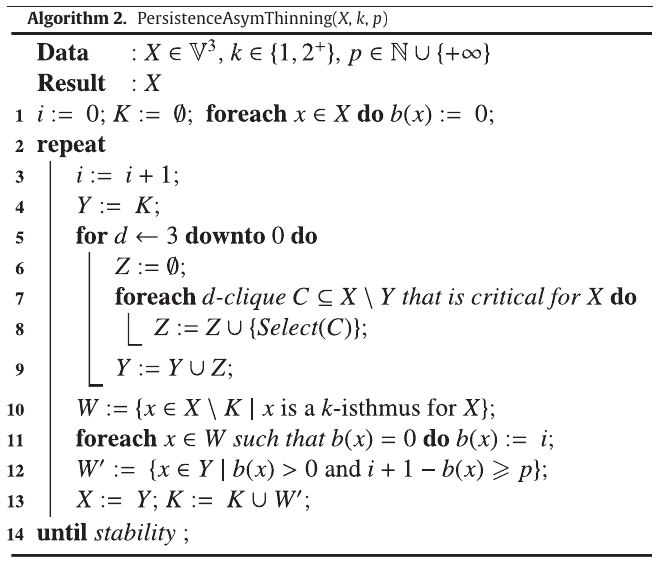
\includegraphics[width=0.8\linewidth]{Figures/chapter-image/dgtal/voxelComplexAlgoPersistence.png}
  \caption{Asymmetric thinning algorithm with persistence, from Ref.~\cite{couprie_asymmetric_2016}}
  \label{fig:algo_persistence}
\end{figure}

Based on this framework, the concept of persistence of a voxel in the thinning \cite{couprie_asymmetric_2016} is implemented. The motivation is to automatically prune those branches that do not belong to a robust skeleton.

Let $i$ be the generation (see \autoref{fig:algo_persistence}) at which a voxel $x$ becomes an isthmus for the first time, we name it \textit{birth date} $b(x) = i$ of the voxel. In a later generation $j$ of the thinning process, the voxel might become deletable, we call it \textit{death date} $d(x) = j$.
The definition of \textit{persistence} of a voxel is the difference between death and birth date, $p(x) = d(x) - b(x)$.
We can choose to only keep isthmuses that have a persistence greater than a selected threshold. This persistence can be interpreted as a relative measure of the elongation of an object. With the persistence parameter, the user decides how much the elongation of an object must exceed its width to be preserved. This effectively prunes short and insignificant branches.

\begin{figure}[!htb]
  \centering
  \begin{subfigure}{0.333\textwidth}
    \centering
    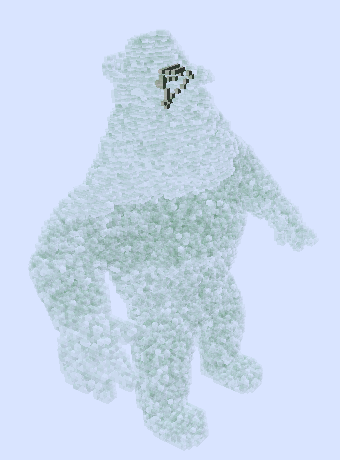
\includegraphics[width=0.95\textwidth]{Figures/chapter-image/dgtal/voxelComplexAlUltiP0.png}%
    \caption{}
    \label{subfig:thin_al_ulti}
  \end{subfigure}%
  \begin{subfigure}{0.333\textwidth}
    \centering
    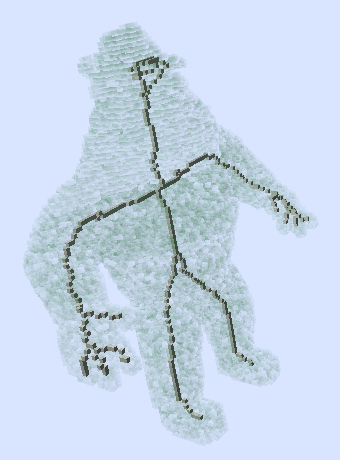
\includegraphics[width=0.95\textwidth]{Figures/chapter-image/dgtal/voxelComplexAl1IsthtmusP0.png}%
    \caption{}
    \label{subfig:thin_al_p0}
  \end{subfigure}%
  \begin{subfigure}{0.333\textwidth}
    \centering
    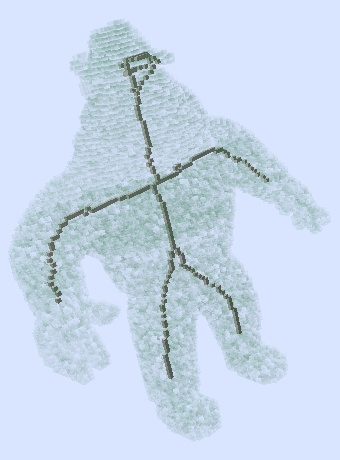
\includegraphics[width=0.95\textwidth]{Figures/chapter-image/dgtal/voxelComplexAl1IsthtmusP10.png}%
    \caption{}
    \label{subfig:thin_al_p10}
  \end{subfigure}
  \caption{Asymmetric thinning of a volume with different parameters. (\subref{subfig:thin_al_ulti}): Ultimate skeleton, only voxels that conserve topology are kept. (\subref{subfig:thin_al_p0}): keeps 1-isthmus as part of the skeleton. (\subref{subfig:thin_al_p10}): 1-isthmus with persistence parameter $p = 10$}
  \label{fig:thin_al}
\end{figure}

The implementation also allows unlimited flexibility, thanks to a functional style, to choose the \textit{Select} and \textit{Skel} function for any purpose.

The \textit{Select} function chooses a voxel from a given pool. This is necessary given the parallel or asymmetric nature of the algorithm. The options are:

\begin{itemize}[topsep=0pt]
  \item \textbf{selectRandom: } Given a set of voxels (a clique), chooses one at random.
  \item \textbf{selectFirst: } Select the first voxel in lexicographical order.
  \item \textbf{selectMaxValue: } Select a voxel with the max value of another user-defined function. This wrap will be used with a distance map (see \autoref{sub:distance_maps}).
\end{itemize}

The \textit{Skel} function provides a way to keep voxels that are wanted to be preserved in the final skeleton.

\begin{itemize}[topsep=0pt]
  \item \textbf{skelUltimate: } Null, only preserve voxels whose removal alters the topology.
   The result of the thinning in a solid object without holes and no branches is just one voxel.
  \item \textbf{skelEnd: } Preserve voxels that have only one neighbor.
  \item \textbf{OneIsthmus: } Preserve 1-isthmus voxels.
  \item \textbf{TwoIsthmus: } Preserve 2-isthmus voxels.
  \item \textbf{skelIsthmus } Preserve 1 and 2-isthmus voxels.
  \item \textbf{skelWithTable } Accepts a look-up-table (LUT) of pre-computed values of certain property for certain configuration of voxels. This is used with pre-computed LUT tables for isthmus to greatly speed up the computation. It is greatly recommended and LUT tables for 26\_6 (fully connected in 3D) topology are provided.
\end{itemize}

\begin{figure}[!htb]
\begin{center}
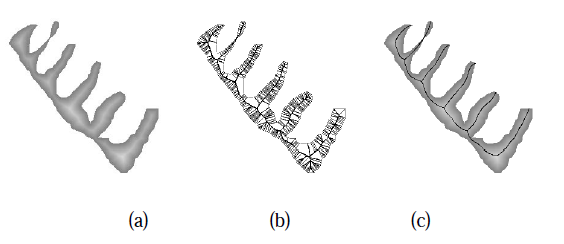
\includegraphics[width=0.8\textwidth]{Figures/chapter-image/skeleton-fixedtopo_letters.png}%
\caption[Skeletonization]{Skeletonization process. (a) Distance
map. (b) Traditional skeleton with no pruning. (c) Skeleton generated using
fixed topology methods. From Ref.\citep{bai_skeleton_2007,golland_fixed_2000}}.
\label{fig:skeleton-fixedtopo}
\end{center}
\end{figure}

The original implementation \cite{couprie_asymmetric_2016} does not ensure obtaining a centered skeleton, but here I introduce the use of a distance map for our \textit{Select} skeletonization function, to first select the voxels which have max value in the distance map. This selects the voxels in the medial axis, obtaining a centered skeleton while keeping the same topology.
To our knowledge, this is the first time where such state of the art digital topology algorithms are applied to biopolymers images.

\section{Spatial Graph Extraction}%
\label{sec:spatial_graph_extraction}

From the skeletonization using the Critical Kernels Framework (see \autoref{sub:critical_kernels_framework}) a thin image is obtained, where all the pixels belonging to an object in the binary image are reduced to a thin representation of it, in the sense that this generated skeleton is one-pixel wide.

From here, our task is to transform this thin image or skeleton into a \gls{graph}. A set of nodes connected to each other through edges. The first step, and also contributed to the DGtal library, is to obtain a \textbf{raw graph}, a graph where each node is a voxel of the skeleton, and neighbor voxels have an edge connecting them.

For regular images, this raw graph is enormous, imagine a voxel in the interior of an object, assuming a fully connected topology, this voxel would be in the center of a $3\times3\times3\times$ cube of voxels, having 26 connected neighbors, i.e. 26 edges or degree = 26. These neighbors voxels are nodes as well, and might be connected to others.
But for thin images, where the number of voxels is greatly reduced, this allow us to start using tools from graph theory to extract a more meaningful graph, a \gls{Spatial Graph}.

In a \gls{Spatial Graph} only nodes with degree different than 2 are considered vertices (see \autoref{fig:spatial_graph}). These end (degree = 1) and junction (degree > 2) nodes are connected to similar nodes via \glspl{Spatial Edge}, where the bending points (degree = 2) connecting those are stored in the spatial edge as \textbf{edge points} (see \autoref{fig:spatial_graph_intro_2} for an example). The rest of vertices are kept with the same connectivity as \glspl{Spatial Node}, adding its index or spatial position from the image.

This transform uses a Depth First Search (\gls{DFS}) visit, starting from end-points vertices (degree=1), it follows the connected neighbors (chain-nodes of degree 2) until it reaches another end-point or another vertex with degree 3 or more. When this happens, two \glspl{Spatial Node} are added to the new \gls{Spatial Graph} (the starting node source and the end node), and one \gls{Spatial Edge}, containing all the visited 2-degree pixels.

The \gls{DFS} algorithm is applied iteratively in the graph, but the visited nodes are marked to avoid re-visiting them. After starting with end-points, it re-starts with any non-visited junction nodes (degree > 2). And to finish, self-loops are discovered, circular structures where all nodes have degree 2. Because the graph doesn't allow self-loops, edges where source and target are the same node. These self-loops are encoded into two nodes, the first is the original vertex, and the second one is created in the median of the \gls{Spatial Edge}. So these self loops are two nodes with two parallel edges of about the same number of edge-points between them.

The \gls{DFS} algorithms is quite fast thanks to its marking of already visited nodes. There are two filters that can be applied to the process that have an impact in the generated \gls{Spatial Graph}.

The original \textbf{Raw Graph} can be optionally post-processed, if there are three nodes with degree 3 connected between them, the longest edges (diagonals) are removed (see \autoref{subfig:graph_raw_merged}).


\begin{figure}[!htb]
  \centering
  \begin{subfigure}{0.5\textwidth}
    \centering
    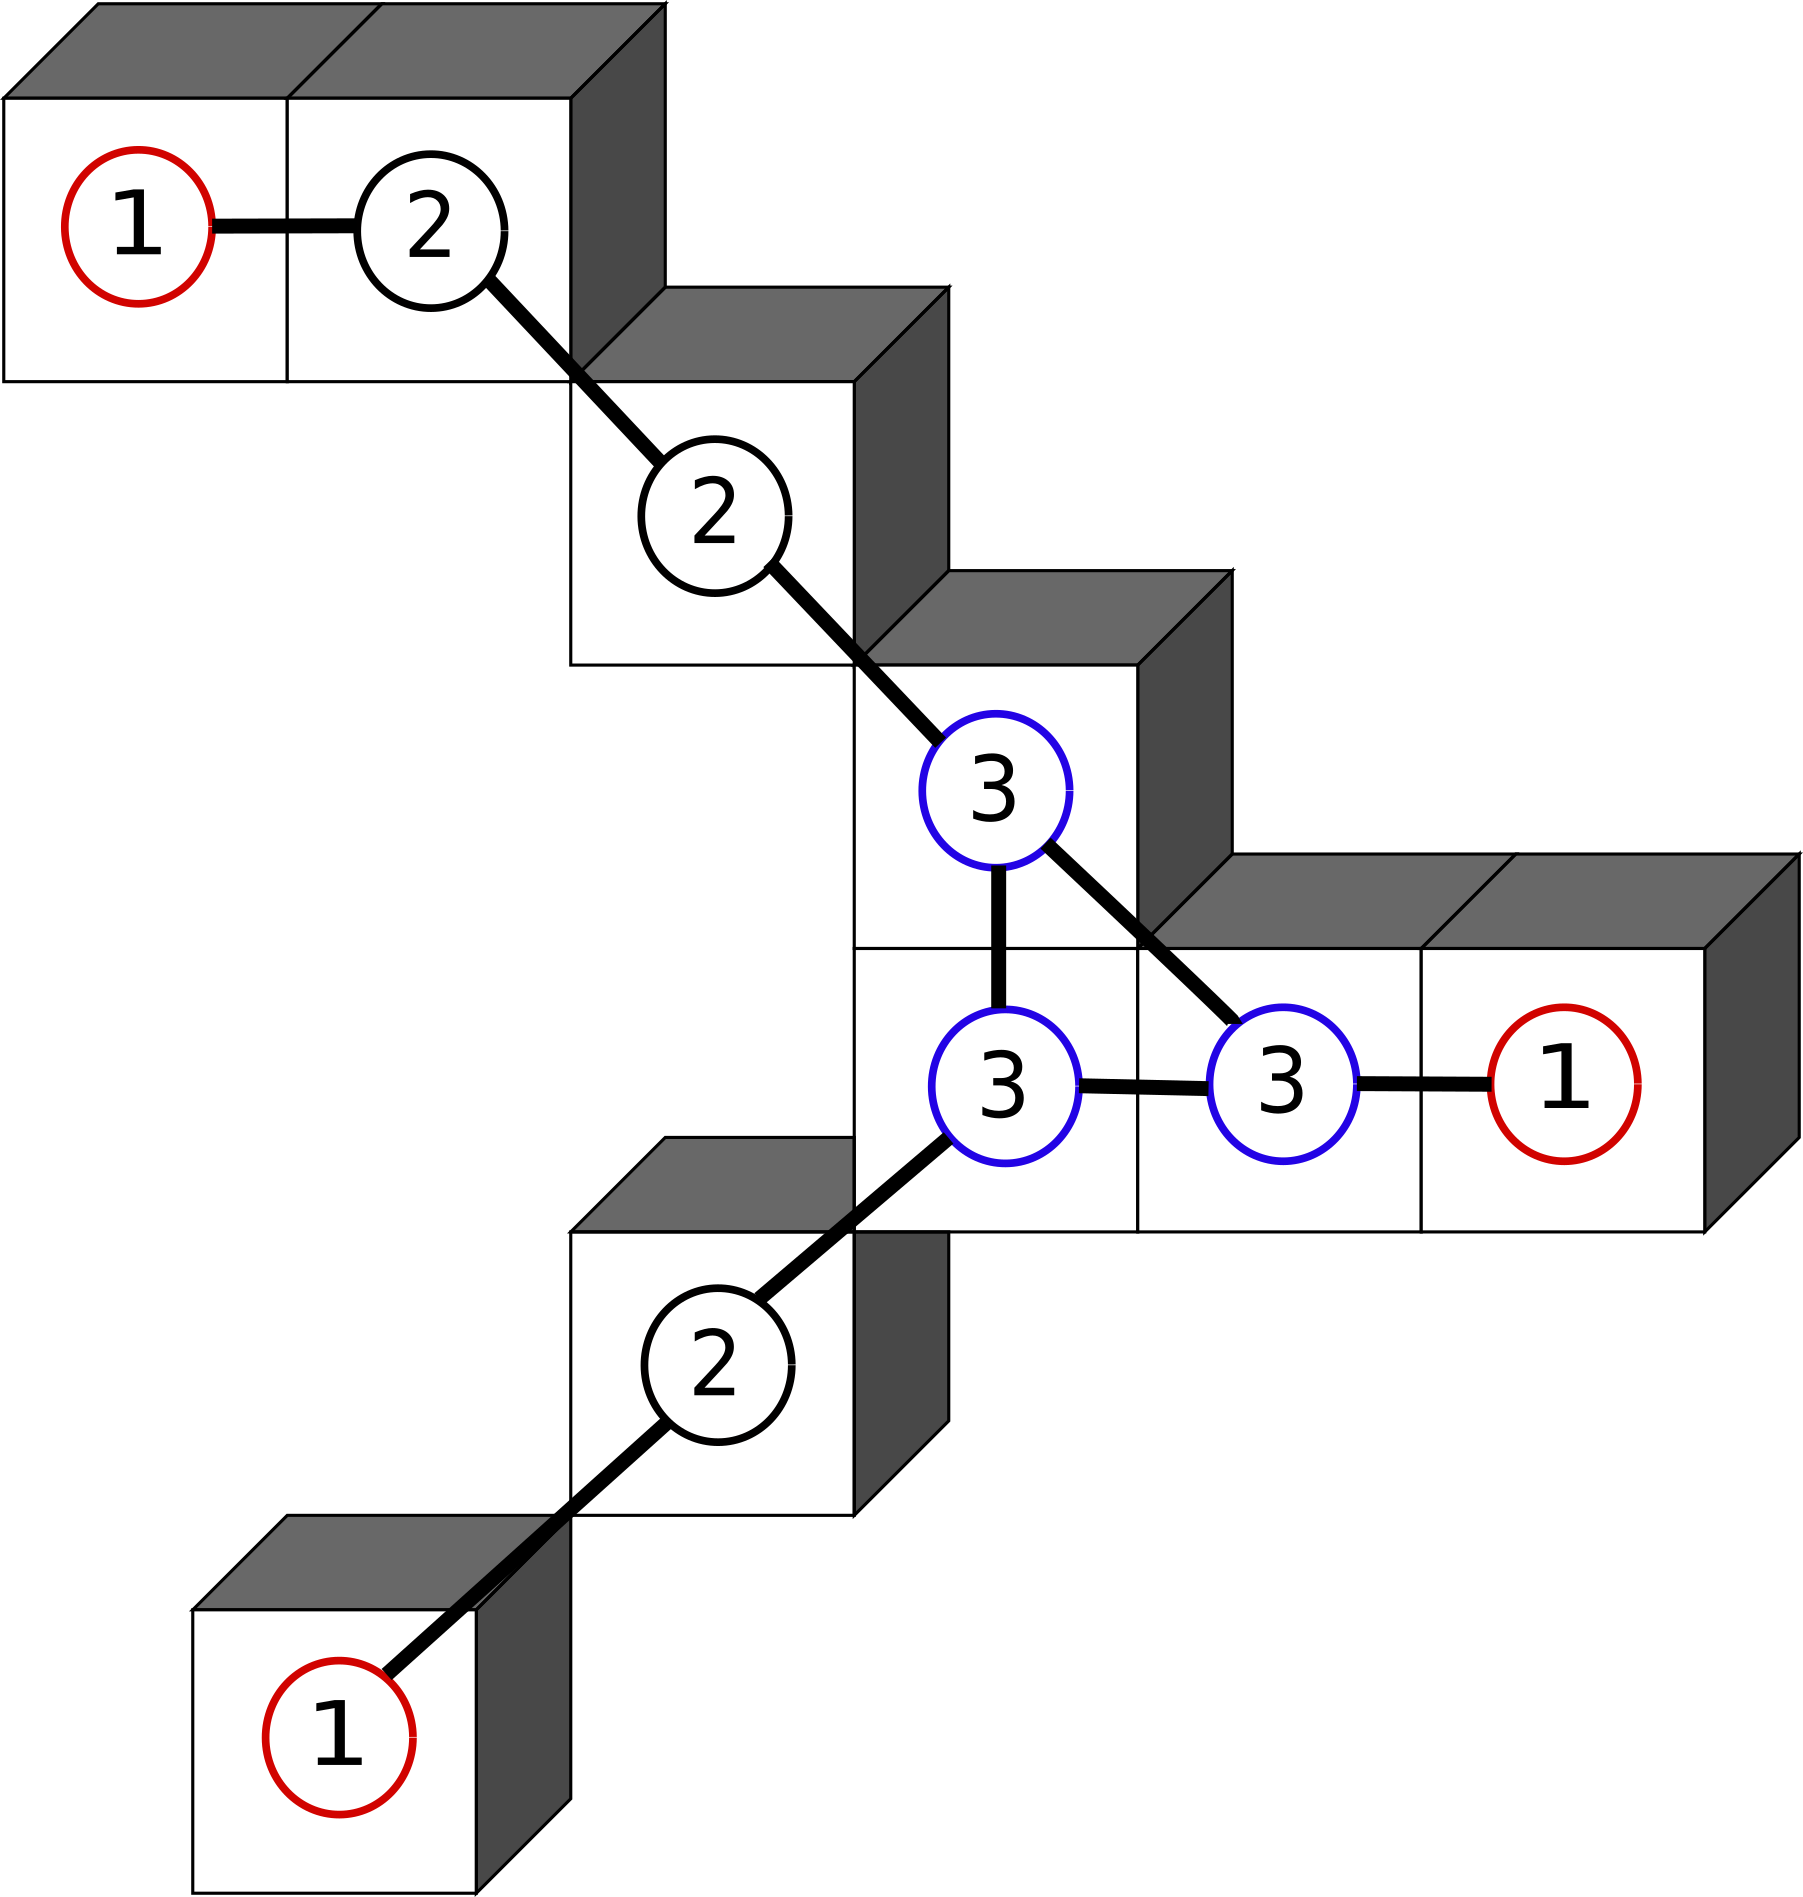
\includegraphics[width=0.9\textwidth]{Figures/chapter-image/dgtal/voxels_raw.png}%
    \caption{Raw Graph.}
    \label{subfig:graph_raw}
  \end{subfigure}%
  \begin{subfigure}{0.5\textwidth}
    \centering
    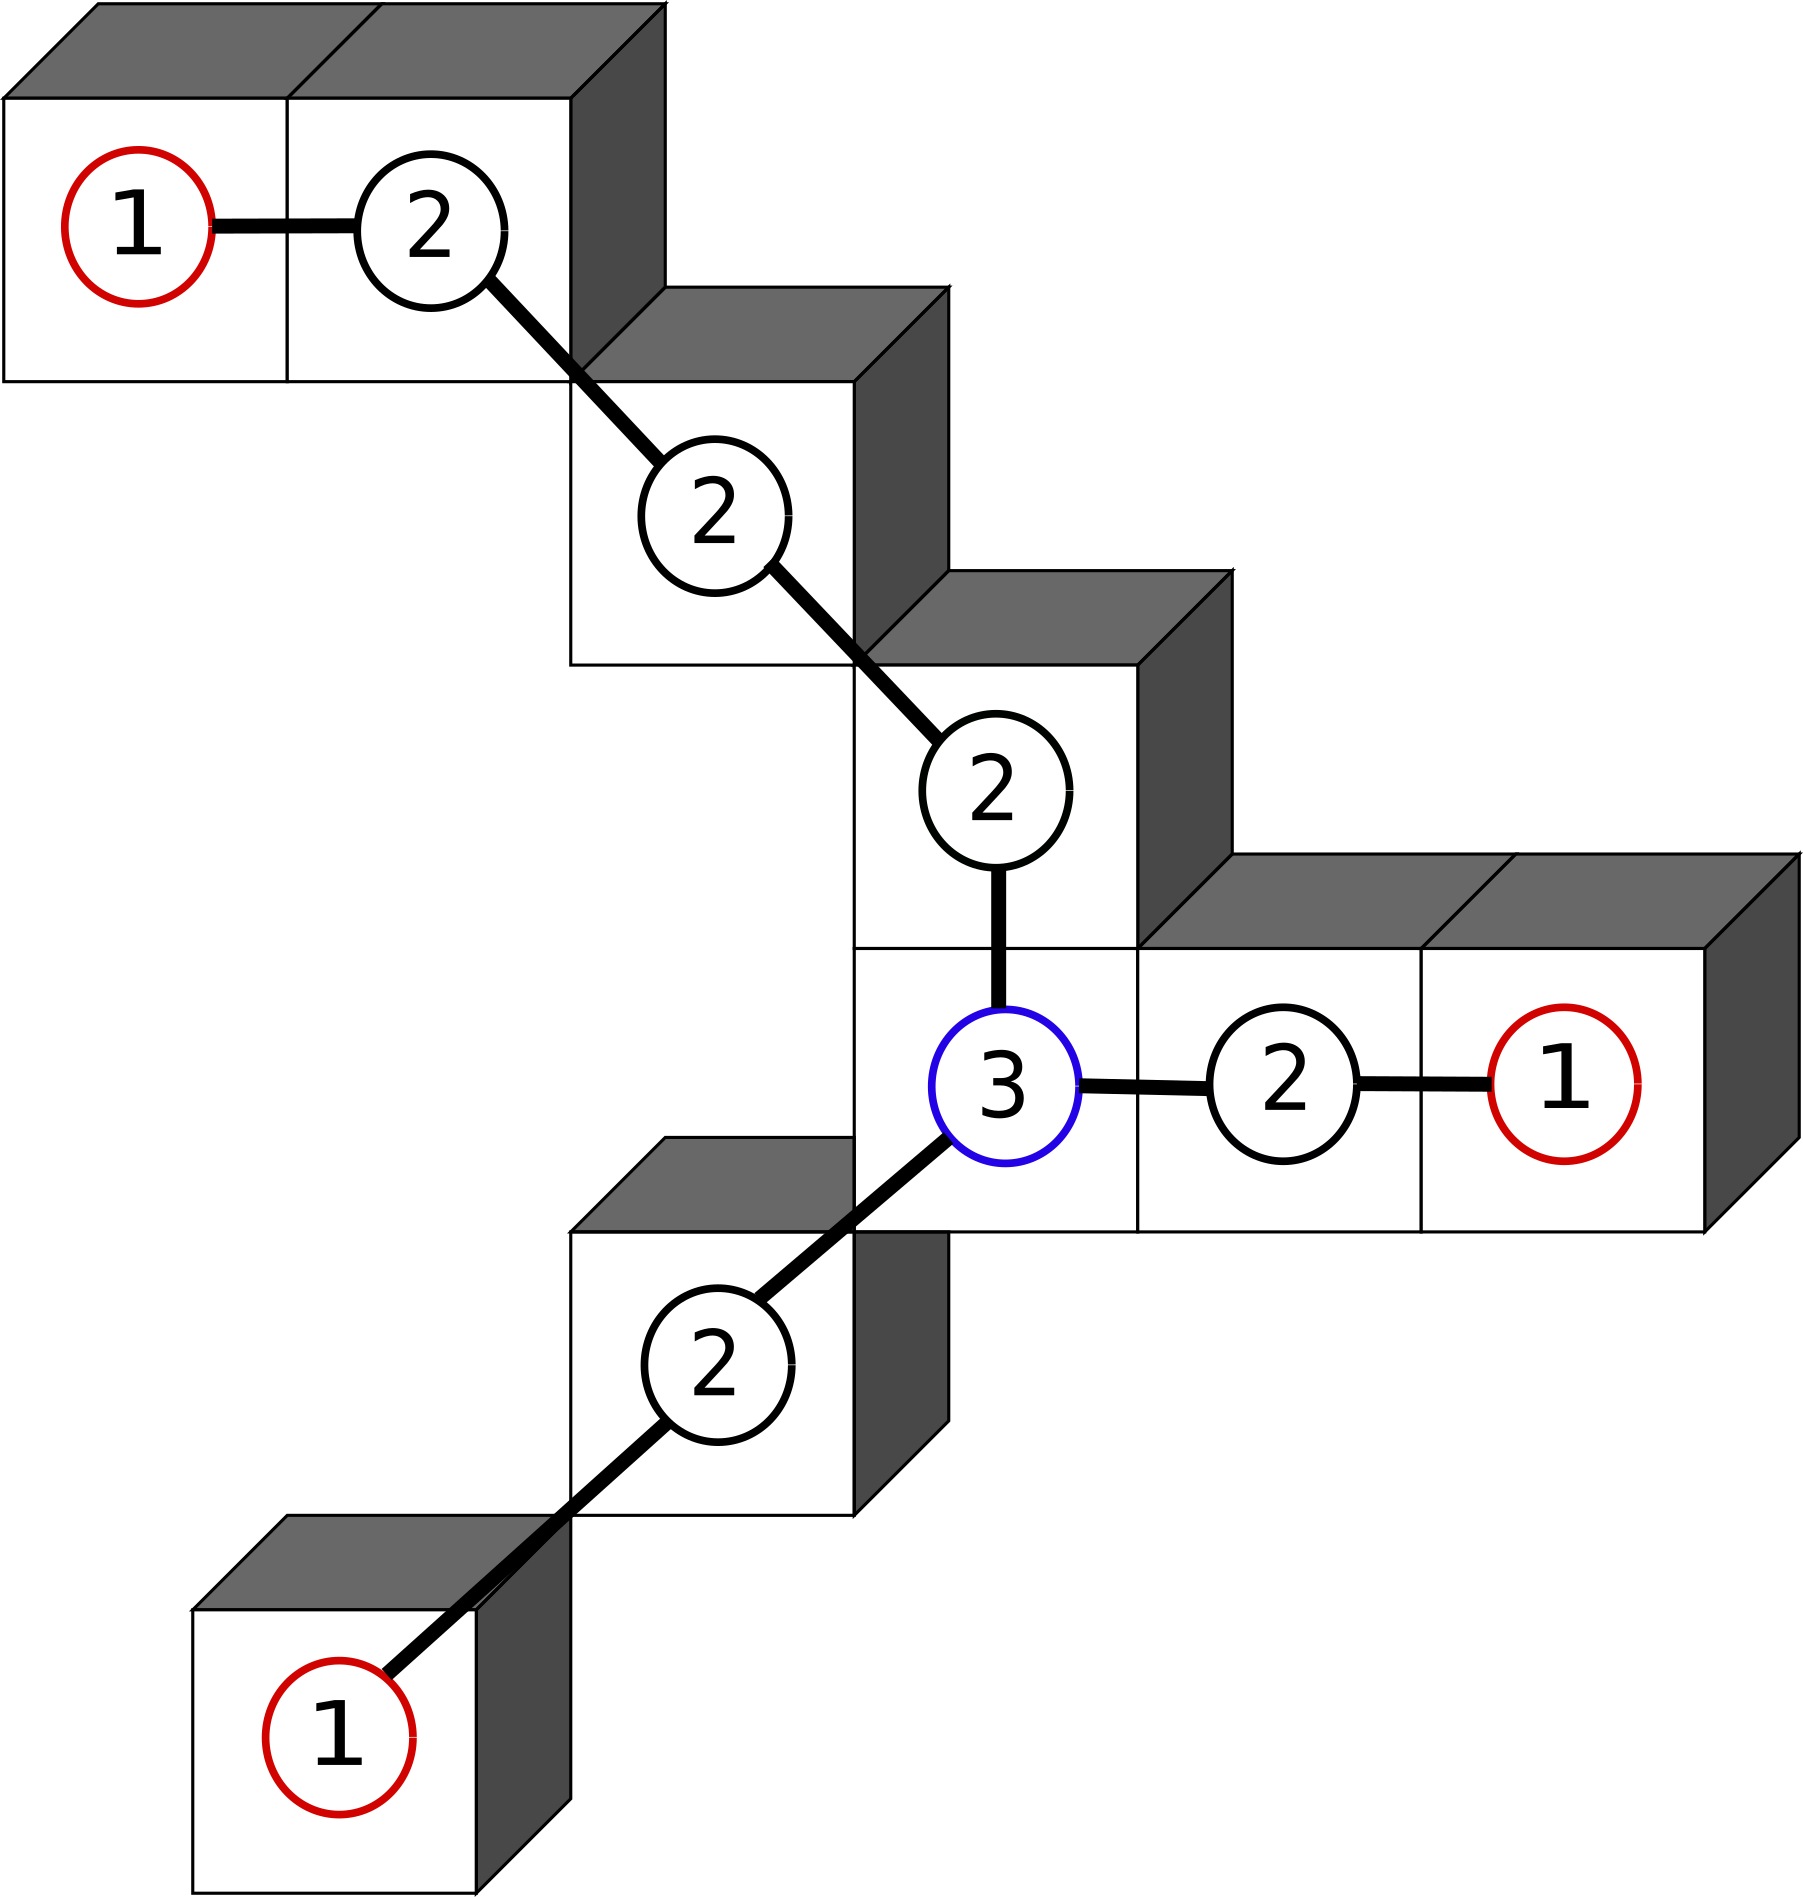
\includegraphics[width=0.9\textwidth]{Figures/chapter-image/dgtal/voxels_raw_merged.png}%
    \caption{Raw Graph merged}
    \label{subfig:graph_raw_merged}
  \end{subfigure}%
  \caption{Extracting the raw graph from the thin image and post processed to remove the largest edges between tri-connected nodes with degree 3. Numbers show the number of edges (degree) of each node. }
  \label{fig:raw_graph_extraction}
\end{figure}


\begin{figure}[!htb]
  \centering
  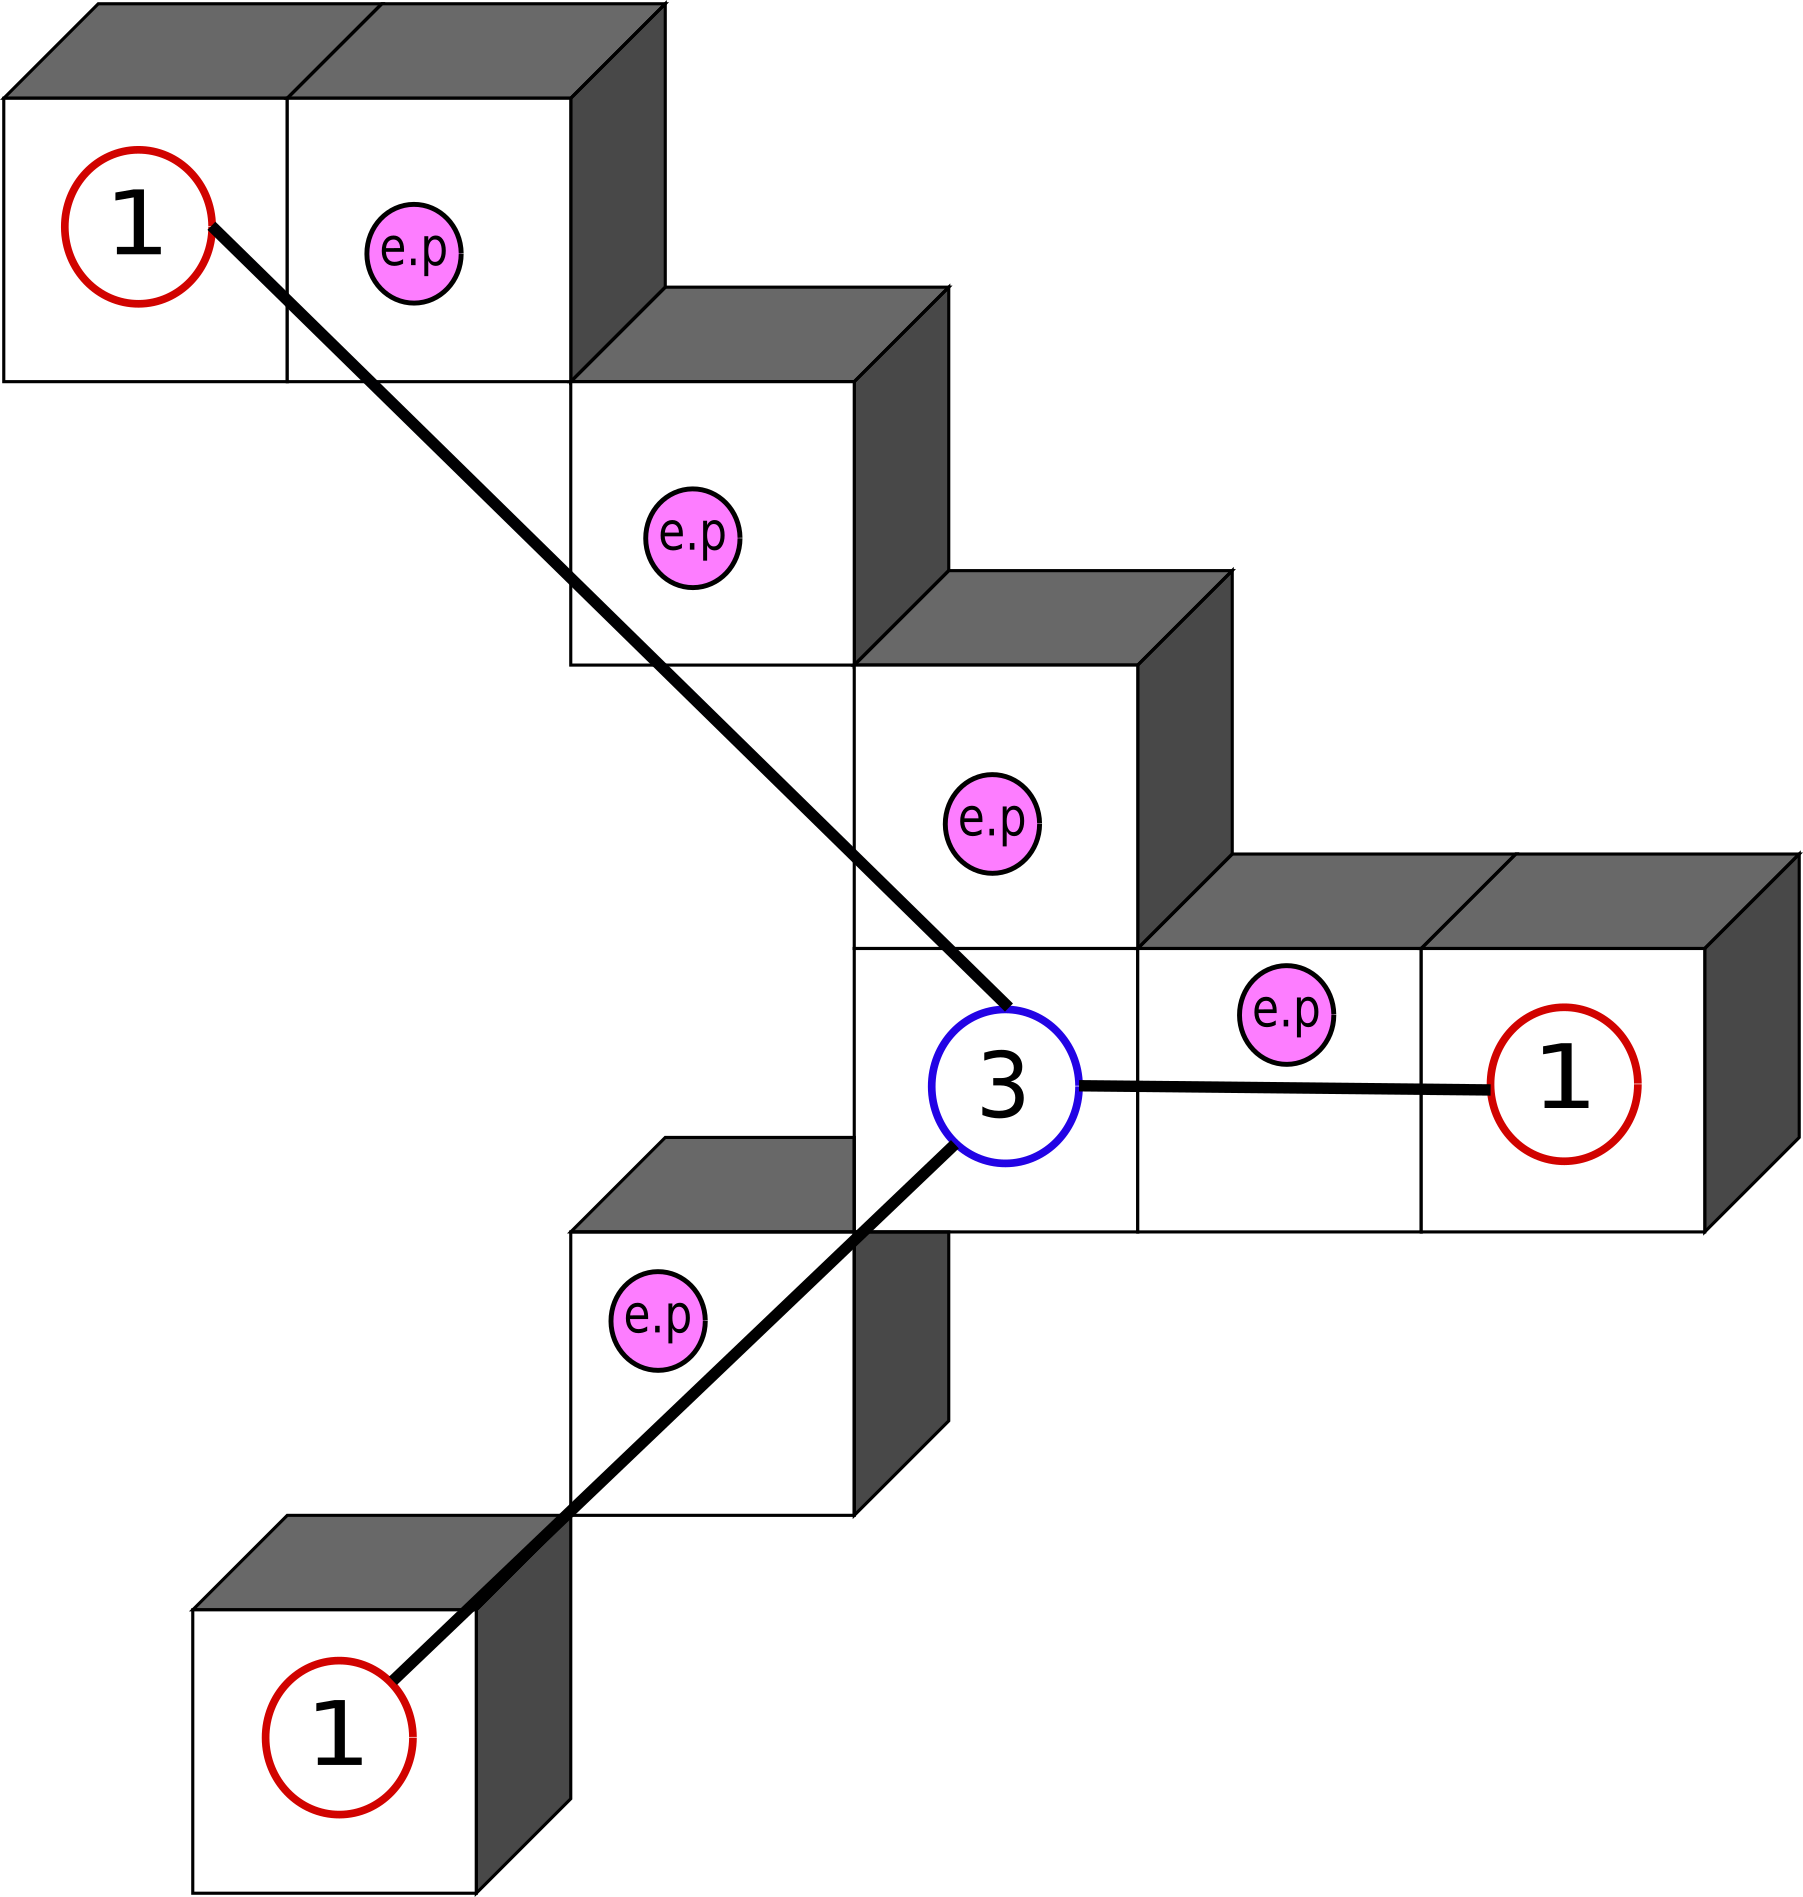
\includegraphics[width=0.45\textwidth]{Figures/chapter-image/dgtal/voxels_spatial_merge.png}%
  \caption{\gls{Spatial Graph} where vertices with degree 2 are deleted, and its position are stored as edge points in the new edges. Numbers in circles represent degree of each node.}
  \label{fig:spatial_graph}
\end{figure}

The spatial graph gives access to the complete network geometry, and additionally allows us to analyze the architecture with sharper tools.

\section{Statistical distributions of graph properties}%
\label{sec:statistical_distributions_of_graph_properties}

With the spatial graph in hand we have at our disposal all the tool-box from the field of
complex networks to characterize the network plus all the geometrical measurements that might be needed due to the storage of positions of each node and edge points in the spatial graph.

Following the approach of Lindstrom to characterize networks from statistical distributions \cite{lindstrom_finite-strain_2013, lindstrom_biopolymer_2010}, the degree distribution, the end-to-end distance between nodes (ignoring edge points), the contour lengths between nodes (taking into account edge points), and the angles between adjacent edges and direction cosines of those angles are computed.

Also any existing short branch can be pruned when computing these properties, the spatial graph won't be affected, only the data extracted from it. Usually, the extremely short branches with only one or two edge points are chosen for removal to have a cleaner vision of the important branches of the network. These really short edges are not significant when getting a broad representation of network properties, but the user decides if and to what extent they are ignored.

For all our networks the degree-distribution can be described by a geometric distribution (see \autoref{degree-dist}), truncated for branch-points (only nodes with degree greater than 3) .

The end-to-end distance between nodes and the contour lengths distributions fits to a
log-normal distribution, see \autoref{length-dist}. This distribution is used to describe multiplicative processes in many fields.
In biology they are used to describe growth processes \cite{mitzenmacher_brief_2004}.

These distributions are the result of the generative processes in network formation, and can be used to infer the details of such processes and patterns \cite{frank_common_2009, frank_how_2014}.

The direction cosines of the angles between adjacent edges is fitted to a truncated power series \cite{lindstrom_finite-strain_2013}, that fits well for all the networks studied, see \autoref{cosines-dist}.


\section{Testing existing thinning algorithms}%
\label{sec:testing_other_thinning_algorithms}

Thinning algorithms have been applied to confocal microscopy images containing biopolymer protein networks before \cite{stein_algorithm_2008, lindstrom_biopolymer_2010}.
In this section I test and describe the algorithms used on these extractions, and discuss why I discarded them and used the recently developed Critical Kernel Framework \cite{bertrand_powerful_2014} described in \autoref{sub:critical_kernels_framework}.

\subsection{FIbeR Extraction -FIRE-}
\label{sub:FIRE}

FIRE has been developed in Matlab by Andrew M. Stein
  \citep{stein_mathematical_2007} to extract collagen networks from confocal
  images. It is an open source application with a BSD licence and it can be downloaded from
  \url{https://github.com/uw-loci/fiber-extraction}. The method
  \citep{stein_algorithm_2008} is based on an original idea of
  \citet{wu_automated_2003}. The main upgrade is the use of multiple nucleation
  points  and the restriction that each branch extends only  in a single
  direction from a nucleation point. In \citet{wu_automated_2003} the network has a single nucleation point at the global maximum of the image distance function D.

 \begin{enumerate}[label=\textbf{\Alph*}]

 \item \textbf{Smooth filter} Smooth the image with a Gaussian filter.
 \item \textbf{Binarization threshold} Keep a percentage of the brightest pixels.
 \item \textbf{Distance map D} Distance map using Euclidean distance. It
 assigns a value to each pixel equal to the distance from that pixel to the nearest black value.

 \item \textbf{Nucleation points NPs} They are the
 local maxima of the distance map $D(\vect{u})$. The locality is defined by a
 box of chosen radius $s_{xbox}=5$. They are only selected if they
 exceed a tunable threshold $\theta_{nuc}=2$. A single nucleation point of
 value $4$ is denoted by the thick circle in \ref{fig:fire_LMPS}\subref{LMP1}.

 \item \textbf{Extension of branches LMPs} The next step is to trace the
 branches, extending from the nucleation points. To do that FIBER finds a set of
 Local Maximum Points (LMPs) at \emph{each} nucleation point. LMPs occur where
 there is a local maximum in $D(\vect{u})$ on the surface of the box centered in the NP
 $\vect{u}$, and with radius(in pixels) the rounded up value of $D(\vect{u})$.
 See Fig. \ref{fig:fire_LMPS}\subref{LMP1}. LMPs are then extended with other
 LMPs only if the direction of extension is straight enough
 (Fig. \ref{fig:fire_LMPS}\subref{LMP2}). If there is no LMP with that
 condition, or it arrives at another nucleation point, the iteration ends.
 \end{enumerate}


\begin{figure}[H]
  \centering
  \begin{subfigure}{0.5\textwidth}
    \centering
    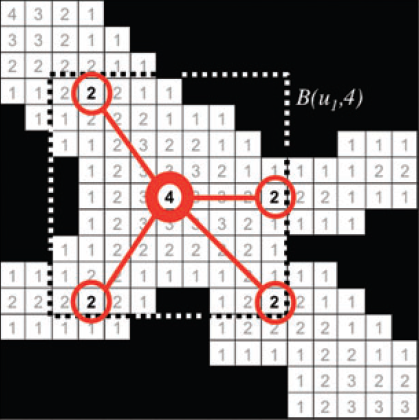
\includegraphics[width=0.8\textwidth]{Figures/chapter-image/fire/nucleation1.png}%
    \caption{Step 1}
    \label{LMP1}
  \end{subfigure}%
  \begin{subfigure}{0.5\textwidth}
    \centering
    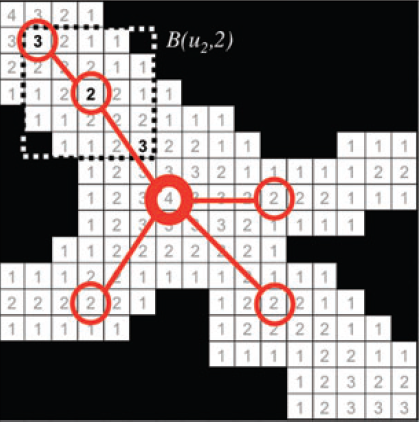
\includegraphics[width=0.8\textwidth]{Figures/chapter-image/fire/nucleation2.png}
    \caption{Step 2}
    \label{LMP2}
  \end{subfigure}
  \caption[FIRE algorithm - Find LMP]{Tracing of the ridges of the distance
    map using FIRE from Ref.\citep{stein_algorithm_2008}: \ref{LMP1} Step 1:
    Pick a nucleation point (thick circle) and find all LMPs. \ref{LMP2} Step 2:
    Pick a LMP and find the next LMP which continues in the same direction. See
  text for details.}
  \label{fig:fire_LMPS}
\end{figure}

\subsubsection{Results in FIRE}
 I have used FIRE to analyse our
 confocal stacks obtained from actin networks. For testing purposes, the images
have been cropped due to the slowness of FIRE
processing big networks, due to being in Matlab and the nature of the algorithm itself.
From an original image of Actin of
$V=1024\times1024\times39$, I have cropped it to $V=200\times200\times20$.

Fig.\ref{fig:fire_stepbystep} shows the different steps of the FIRE
algorithm. In Fig.\ref{fig:fire_histograms} a plot is shown with the statistical distribution
of end-to-end distances and degree for different thresholds $T_P$.
These distributions will be further discussed in \autoref{sec:statistical_distributions_of_graph_properties} and \autoref{Chapter-Reconstruction}.

The drawback of FIRE is that the topology of the networks is not guaranteed to be conserved in the extracted skeleton. Some branches could be missed depending of its parameters,
and noisy skeletons are generated. These are restrictions inherited from the algorithm originally developed in 2003 \cite{wu_automated_2003}.
The other drawback is that is developed for Matlab which is designed for fast prototyping of algorithms, but the speed of the computations is compromised without further optimizations. Even though the software is open source, it requires that users own a license of Matlab to run the algorithm.

\begin{figure}[H]
  \centering
  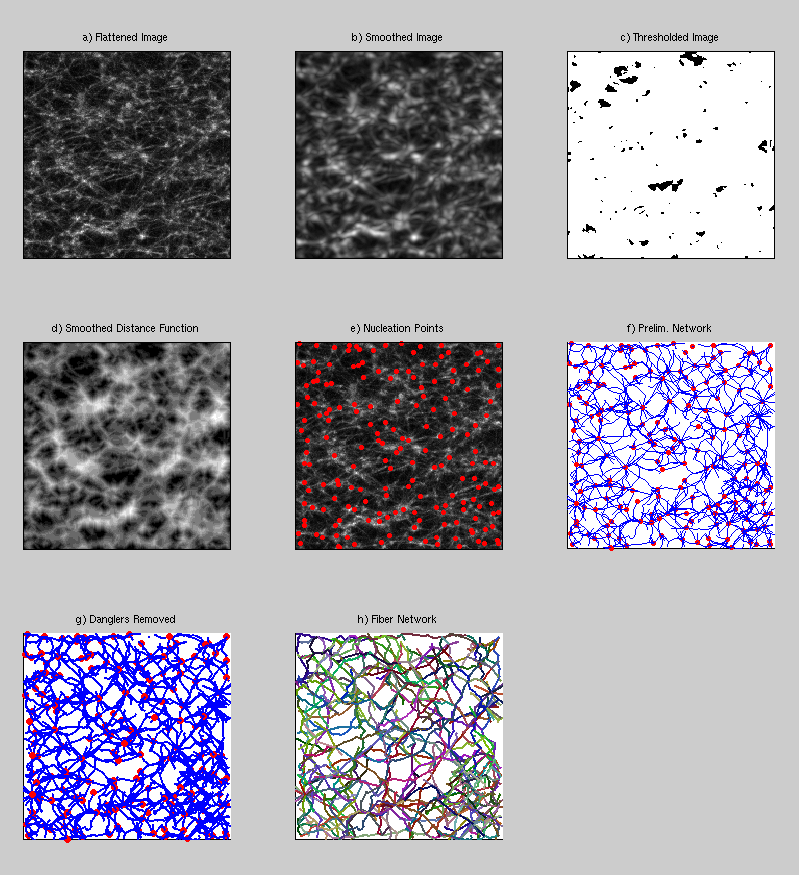
\includegraphics[width=0.9\textwidth]{Figures/chapter-image/fire/fire012.png}%
  \caption[Fire: Step by step for $T_P=0.12$]{FIRE: step by step}
  \label{fig:fire_stepbystep}
\end{figure}

\begin{figure}[H]
  \centering
  \begin{subfigure}{0.5\textwidth}
    \centering
    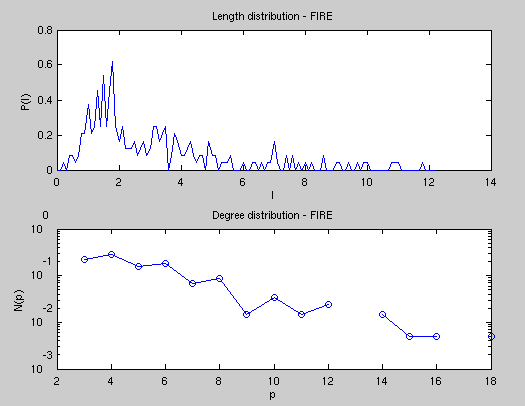
\includegraphics[width=0.95\textwidth]{Figures/chapter-image/fire/fire017histo.png}%
    \caption{$T_P=0.17$}
    \label{firehisto017}
  \end{subfigure}%
  \begin{subfigure}{0.5\textwidth}
    \centering
    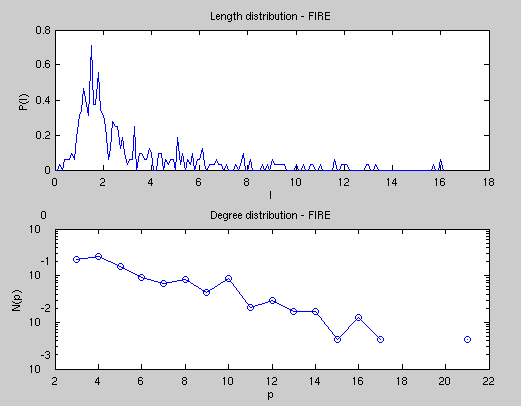
\includegraphics[width=0.95\textwidth]{Figures/chapter-image/fire/fire012histo.png}%
    \caption{$T_P=0.12$}
    \label{firehisto012}
  \end{subfigure}

  \begin{subfigure}{0.5\textwidth}
    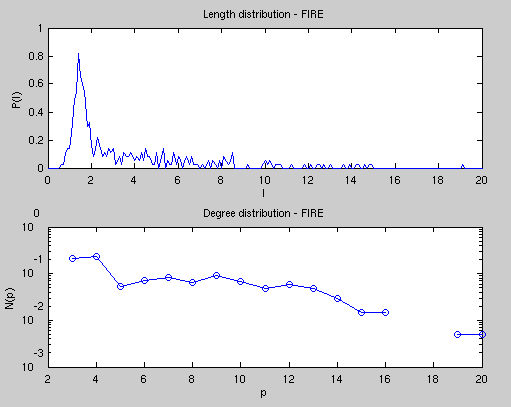
\includegraphics[width=0.95\textwidth]{Figures/chapter-image/fire/fire008histo.png}%
    \caption{$T_P=0.08$}
    \label{firehisto008}
  \end{subfigure}
\caption[Distributions of length and degree in FIRE]{Extracting statistical
distributions for different binary thresholds using FIRE from cropped
actin netwoks.}
\label{fig:fire_histograms}
\end{figure}

% A useful statistical distribution is the one studying the angles between edges
% that are incident to the same node. I am currently working on a way to extract
% the direction cosines (angles) distribution from FIRE.

\subsection{Avizo: XSkeleton}
\label{sub:avizo}
 Avizo is a software commercialized by
 \href{http://www.vsg3d.com/avizo/overview}{FEI: Visualization Sciences Group}.
Access to Avizo was obtained through a collaboration with Fonterra (Food company,
NZ).

Avizo uses a Distance Ordered Homotopic Thinning (DOHT) algorithm, that ensures homotopy (i.e. keeps the same topology than the original object),
thinness and centered skeletons.

\textbf{XSkeleton} is the package or module that used to extract the
network topology. The algorithm and the result are different to FIRE. Here
follows a description step by step:
\begin{enumerate}[label=\textbf{\Alph*}]
 \item\textbf{Smooth filter} Smooth the image with a Gaussian filter
 \item\textbf{Binarization threshold} Multi-threshold module. This threshold is
 not based in percentage of the brightest pixel. It is a classical threshold turning
 to pure white $255$ all pixels with a value greater than the
 threshold value, and black all the pixels below that value.
 \item\textbf{Distance map} Distance map using Euclidean distance. It assigns a
 value to each pixel equal to the distance from that pixel to the nearest black value.
 \item\textbf{Thinner module} This is the \textbf{skeletonization} step. The
 module takes as input a label-field to be thinned and a distance map scalar field. It removes voxel by voxel from the segmented
 object until only a string of connected voxels remains.
 The thinning algorithm automatically detects dead end branches of skeleton
 spatial graphs. A parameter is used to distinguish them from noise on the
 interface  of the considered regions to avoid spurious branches.  Its default
 value is 5, i.e. the branches with a dead end which length is lower  than 5
 voxels are automatically considered as noise and removed.  Setting this to 10,
 which is a rather large value, leads to only a few branches remaining in the
 skeleton.  The drawback is that you also might miss real endpoints.

\item\textbf{Trace lines module} Converts an image that contains lines
represented by voxels into a spatial graph object.

 \end{enumerate}

\begin{figure}[H]

% \begin{minipage}{0.5\textwidth}

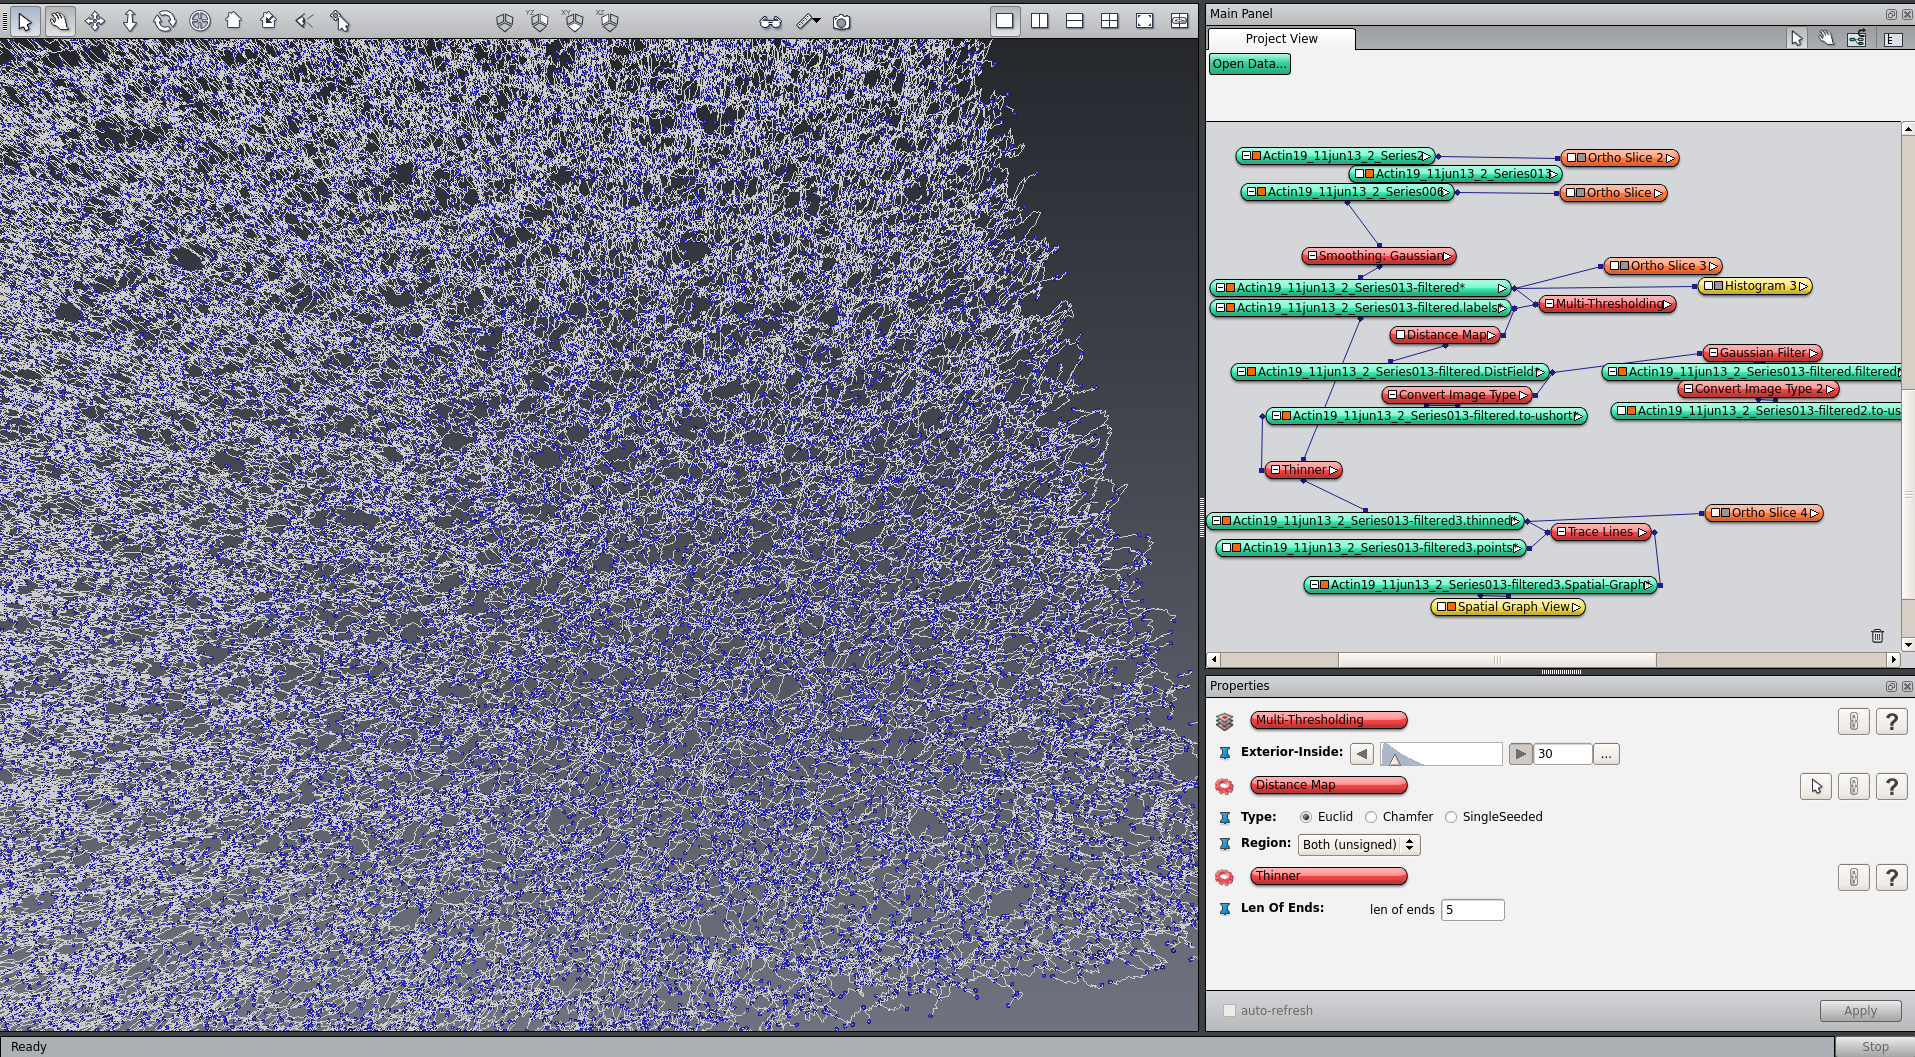
\includegraphics[width=0.9\textwidth]{Figures/chapter-image/avizo/workspace-wholedata.png}%

\caption[Avizo image: Actin network visualization and workspace]{Avizo
workspace. \emph{Left:} Visualization of the whole network of Actin data.
\emph{Top right:} Filters applied step by step. \emph{Bottom right:} Most
influential filters parameters, binarization threshold ($30$ in the image) and
skeletonization parameter: pruning of branches that length is lesser than the
threshold ($5$ in the image)}
\label{fig:avizo_workspace}
\end{figure}


\subsubsection{Avizo results:}
The whole stack of our confocal images of actin
($V=1024\times1024\times39$) is analyzed. The key parameters in Avizo are the binarization
$T$ and the pruning threshold $P$.

In Fig.\ref{fig:avizo_workspace}, a regular workspace in Avizo can be seen. The
different filters, the key parameters, and the result of the process, the actin
network are visualized.

In Fig.\ref{fig:avizo_histograms30} the statistical distributions are extracted
from the network that will be used in chapter \ref{Chapter-Reconstruction} for
the reconstruction of the network.

Fig.\ref{fig:avizo_histograms21} shows that statistical distributions
are quite robust versus small changes in the key parameters $T$ and $P$.

\begin{figure}[H]
  \centering
  \begin{subfigure}{0.5\textwidth}
    \centering
    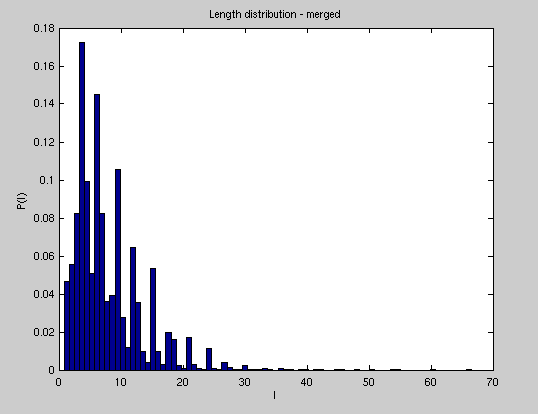
\includegraphics[width=0.92\textwidth]{Figures/chapter-image/avizo/ActinZ39b21l5-histo-length.png}%
    \label{avizo305-length}
  \end{subfigure}\\[1ex]
  \begin{subfigure}{0.5\textwidth}
    \centering
    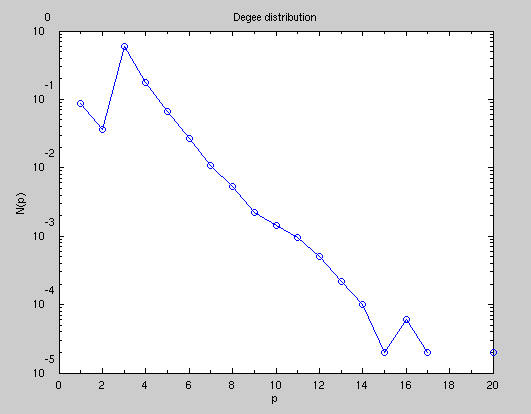
\includegraphics[width=0.92\textwidth]{Figures/chapter-image/avizo/ActinZ39b21l5-histo-degree.png}%
    \label{avizo305-degree}
  \end{subfigure}\\[1ex]
  \begin{subfigure}{0.5\textwidth}
    \centering
    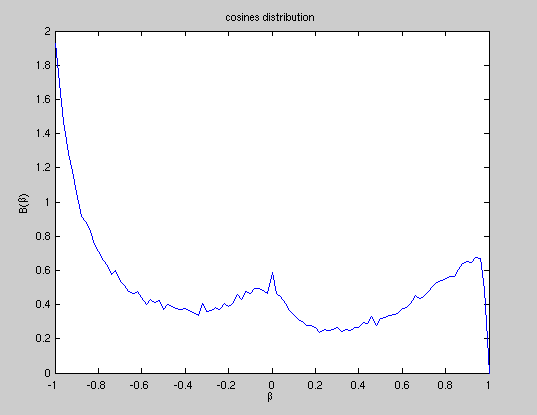
\includegraphics[width=0.92\textwidth]{Figures/chapter-image/avizo/ActinZ39b21l5-histo-cosines.png}
    \label{avizo305-cosines}
  \end{subfigure}

  \caption[Distributions of length, degree, and cosines with Avizo for
  actin with T=30,P=5]{Actin data analyzed with Avizo with binary threshold
    $T=30$ and pruning parameter $P=5$. \subref{avizo305-length} Length following a
    log-normal or exponential distribution. \subref{avizo305-degree} Degree
    following a geometrical distribution. \subref{avizo305-cosines}  Direction
  cosines following an unknown distribution.}
  \label{fig:avizo_histograms30}
\end{figure}

\begin{figure}[H]
  \centering
  \begin{subfigure}{0.45\textwidth}
    \centering
    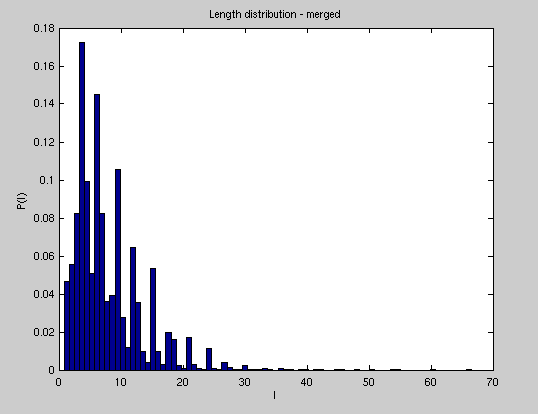
\includegraphics[width=0.92\textwidth]{Figures/chapter-image/avizo/ActinZ39b21l5-histo-length.png}%
  \end{subfigure}
  \begin{subfigure}{0.45\textwidth}
    \centering
    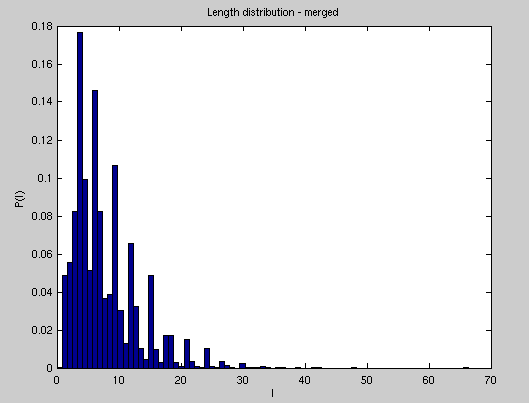
\includegraphics[width=0.92\textwidth]{Figures/chapter-image/avizo/ActinZ39b21l8-histo-length.png}%
  \end{subfigure}\\[1ex]
  \begin{subfigure}{0.45\textwidth}
    \centering
    \includegraphics[width=0.92\textwidth]{Figures/chapter-image/avizo/ActinZ39b21l5-histo-degree.png}%
  \end{subfigure}
  \begin{subfigure}{0.45\textwidth}
    \centering
    \includegraphics[width=0.92\textwidth]{Figures/chapter-image/avizo/ActinZ39b21l8-histo-degree.png}%
  \end{subfigure}\\[1ex]
  \begin{subfigure}{0.45\textwidth}
    \centering
    \includegraphics[width=0.92\textwidth]{Figures/chapter-image/avizo/ActinZ39b21l5-histo-cosines.png}%
  \end{subfigure}
  \begin{subfigure}{0.45\textwidth}
    \centering
    \includegraphics[width=0.92\textwidth]{Figures/chapter-image/avizo/ActinZ39b21l8-histo-cosines.png}%
  \end{subfigure}

\caption[Distributions of length, degree, and cosines with Avizo for
actin with T=21,P=5]{Actin data analyzed with Avizo with binary threshold
$T=21$ and pruning parameter: $P=5$ in the first column, and  $P=8$ in the second
column. It can be appreciated that small changes in the parameters
do not have much effect much on the statistical distributions.}
\label{fig:avizo_histograms21}
\end{figure}

% The statistical distribution must be further compared with those in FIRE (with
% a whole network), but we can see that the algorithm seems stable against minor
% changes in the important parameters.

The parallel implementation of the skeletonization in Avizo, based on \cite{fouard_skeletonization_2004}, makes it very fast even for big volumetric images.
The main drawbacks are two: firstly the algorithm generates spurious branches in noisy contours,
these can be mitigated a-posteriori with the pruning parameter $P$, but with the high risk of missing significant branches.
Secondly, the cost of the licence for Avizo and the needed Skeletonization package is at the range of more than fifty thousands \$ per year. The exact price is not disclosed, and may vary from the packages and user cases, but it effectively makes this skeletonization only available for big institutions or industries.

\section{Application of the Network Analysis Pipeline to Different Biopolymer Networks.}%
\label{sec:sg_results}

% \subsubsection{Comparison with the Critical Kernels Framework}%
% \label{subsub:comparison}

I chose to implement the critical kernel framework from \citep{bertrand_powerful_2014} for biopolymer networks extraction instead of the mentioned cases to use bleeding edge algorithms from the digital topology research community in an open source format, available for any researcher to use. Being based on isthmuses instead of simple points makes it much more resilient against noise and the persistence parameter effectively removes the remaining small spurious branches. In fact, the algorithm ranks first in a quantitative evaluation of the robustness of thinning algorithms \cite{bertrand_powerful_2014, couprie_3d_2015}.

The following pipeline is applied: denoising, binarization, skeletonization, extracting the spatial graph and fitting statistical distributions described in previous sections to three sets of volumetric images, obtained for three different biopolymer networks, and from the two most common 3D imaging modalities.

\begin{itemize}[topsep=0pt]
  \item \textbf{Actin: } Stack of images from Confocal Light Microscopy.
  \item \textbf{Carrageenan: } Image from \gls{TEM} tomography.
  \item \textbf{Pectin: } Image from \gls{TEM} tomography.
\end{itemize}

\subsection{Confocal Light Microscopy: Actin}%
\label{sub:actin}

The actin network studied was prepared using 0.3 mg/ml actin in 40 mMol MgCl2 and stained with phalloidin.
The images were taken using Confocal Laser Scanning Microscopy (CLSM) with a Leica Instrumentat (model TCS SP5).

The volumetric image used in this study has a size of 1024$\times$1024$\times$106 pixels, with resolution 0.505$\times$0.505$\times$1.0070 \si{\micro\metre} per pixel.
%0.505050745877353$\times$0.505050745877353$\times$1.00708103855232 \si{\micro\metre} per pixel.

The parameters used in the image pipeline:

\textbf{Denoise:}

\noindent Using the c++ script \citetitle*{phcerdan_rieszwaveletphaseanalysis_2018} \cite{phcerdan_rieszwaveletphaseanalysis_2018}.
\begin{minted}{bash}
export WAVELET_TYPE=Simoncelli # options: Held, Vow, Shannon
export LEVELS=4
export BANDS=4
rieszWaveletPhaseAnalysis -i ${INPUT_IMAGE} -o ${OUTPUT_FOLDER} \
       -w ${WAVELET_TYPE} -l ${LEVELS} -b ${BANDS}
\end{minted}

I apply an anisotropic denoise step with the itk filter CurvatureAnisotropicDiffusion,
using the python script  \citetitle*{phcerdan_denoise_input_2018} \cite{phcerdan_denoise_input_2018}.

\begin{minted}{bash}
export DENOISE_ITERATIONS=20
export DENOISE_CONDUCTANCE=2.0
export DENOISE_TIMESTEP=0.0625 #default optimal value for 3D
python denoise_input.py ${OUTPUT_WAVELET} ${OUTPUT_FOLDER} \
      ${DENOISE_ITERATIONS} ${DENOISE_CONDUCTANCE}
\end{minted}

Result: \autoref{fig:actin_denoised}.

\textbf{Segmentation:}
Apply a region growing algorithm as explained in \autoref{subsub:region_growing_segmentation},
using the c++ script  \citetitle*{phcerdan_regionGrowingSegmentation_2018} \cite{phcerdan_regionGrowingSegmentation_2018}.
\begin{minted}{bash}
export BIN_RG_LOWER=0.0
export BIN_RG_UPPER=5000
export BIN_SAFE_PERCENTAGE=0.2
regionGrowingSegmentation -i ${OUTPUT_DENOISE} -o ${OUTPUT_FOLDER}\
    -l ${BIN_RG_LOWER} -u ${BIN_RG_UPPER} -p ${BIN_SAFE_PERCENTAGE}
\end{minted}

And the hole filling algorithm described in \autoref{sub:hole_filling},
using the python script  \citetitle*{phcerdan_binary_denoise_3d_fillholes_iterative_2018} \cite{phcerdan_binary_denoise_3d_fillholes_iterative_2018}.

\begin{minted}{bash}
export HOLE_MAJORITY=3
export HOLE_RADIUS=1
export HOLE_ITERATIONS=10000
python binary_denoise_3d_fillholes_iterative.py ${OUTPUT_BINARY} ${OUTPUT_FOLDER}\
${HOLE_MAJORITY} ${HOLE_RADIUS} ${HOLE_ITERATIONS}
\end{minted}

Result: \autoref{fig:actin_segmentation}.

\textbf{Skeletonization}

Apply a thinning using the critical kernels framework contributed to DGtal (see \autoref{sub:critical_kernels_framework})
using the c++ script  \citetitle*{phcerdan_thin_2018} \cite{phcerdan_thin_2018}.

\begin{minted}{bash}
export SKEL_SELECT=dmax
export SKEL_TYPE=1isthmus
export SKEL_PERSISTENCE=2
thin --input ${OUTPUT_SEGMENTATION} -o ${OUTPUT_FOLDER} \
  --select ${SKEL_SELECT} --skel ${SKEL_TYPE} \
  -p ${PERSISTENCE} --foreground white
\end{minted}

The option \textit{dmax} generates a distance map as shown in \autoref{subfig:actin_dmap}.

Result: \autoref{subfig:actin_skeleton}.

\textbf{Spatial Graph Extraction}

The conversion from the thin image to the spatial graph representation as described in \autoref{sec:spatial_graph_extraction},
uses the c++ script  \citetitle*{phcerdan_analyze_graph_2018} \cite{phcerdan_analyze_graph_2018}.

\begin{minted}{bash}
export GRAPH_IGNORE_SHORT_EDGES=1
export GRAPH_SPACING="5.05050745877353E-07 5.05050745877353E-07 1.00708103855232E-06"
analyze_graph --input ${OUTPUT_SKELETONIZATION} \
 --exportReducedGraph ${OUTPUT_FOLDER} --exportData ${GRAPH_DATA_FOLDER}
 --reduceGraph --removeExtraEdges  --mergeThreeConnectedEdges \
 --ignoreAngleBetweenParallelEdges \
 --ignoreEdgesShorterThan ${GRAPH_IGNORE_SHORT_EDGES} \
 --spacing ${GRAPH_SPACING}
\end{minted}

\textit{exportData} computes the graph properties: degree, end-to-end distances, contour lengths, angle and direction cosines, and saves them into a file.

\textit{exportReducedGraph} outputs the spatial graph in a .dot (graphviz) format, similar to \autoref{fig:spatial_graph_intro_2}, that can be read by any graph library.

\textit{removeExtraEdges} applies the removal of diagonal edges at intersections, as described in \autoref{subfig:graph_raw_merged}.

The result is a spatial graph. \autoref{fig:actin_graph} shows a representation of that graph without representing contour lengths, instead lines are just straight lines connecting end-to-end nodes. Node glyphs are not represented to avoid cluttering the 3D scene.


% \begin{minted}{bash}
% # Wavelet Phase Analysis
% export WAVELET_TYPE=Simoncelli
% export LEVELS=4
% export BANDS=4
% # Anisotropic Denoise
% export DENOISE_ITERATIONS=20
% export DENOISE_CONDUCTANCE=2.0
% export DENOISE_TIMESTEP=0.0625
% ## Region Growing Binarization
% export BIN_RG_LOWER=0.0
% export BIN_RG_UPPER=5000
% export BIN_SAFE_PERCENTAGE=0.2
% ## Hole Filling
% export HOLE_MAJORITY=3
% export HOLE_RADIUS=1
% export HOLE_ITERATIONS=10000
% ## Skeletonization
% export SKEL_SELECT=dmax
% export SKEL_TYPE=1isthmus
% export SKEL_PERSISTENCE=2
% ## Spatial Graph Extraction
% export GRAPH_IGNORE_SHORT_EDGES=1
% export GRAPH_SPACING=""
% \end{minted}


% \begin{figure}[!htb]
\begin{figure}[H]
  \centering
  \begin{subfigure}{0.5\textwidth}
    \centering
    \includegraphics[width=0.9\linewidth]{Figures/chapter-image/pipeline_screenshots/actin_volume.png}
    \caption{Original volume.}
    \label{fig:actin_original}
  \end{subfigure}%
  \begin{subfigure}{0.5\textwidth}
    \centering
    \includegraphics[width=0.9\linewidth]{Figures/chapter-image/pipeline_screenshots/actin_denoised_wavelet_anisotropic.png}
    \caption{Denoised.}
    \label{fig:actin_denoised}
  \end{subfigure}\\[1ex]
  \begin{subfigure}{0.5\textwidth}
    \centering
    \includegraphics[width=0.9\linewidth]{Figures/chapter-image/pipeline_screenshots/actin_segmented_sparse.png}
    \caption{Segmentation.}
    \label{fig:actin_segmentation}
  \end{subfigure}%
  \begin{subfigure}{0.5\textwidth}
    \centering
    \includegraphics[width=0.9\linewidth]{Figures/chapter-image/pipeline_screenshots/actin_dmap.png}
    \caption{Distance Map.}
    \label{subfig:actin_dmap}
  \end{subfigure}\\[1ex]
  \begin{subfigure}{0.5\textwidth}
    \centering
    \includegraphics[width=0.9\linewidth]{Figures/chapter-image/pipeline_screenshots/actin_skeleton.png}
    \caption{Skeletonization (p = 2).}
    \label{subfig:actin_skeleton}
  \end{subfigure}%
  \begin{subfigure}{0.5\textwidth}
    \centering
    \includegraphics[width=0.9\linewidth]{Figures/chapter-image/pipeline_screenshots/actin_graph.png}
    \caption{Graph.}
    \label{fig:actin_graph}
  \end{subfigure}%
  \caption{Actin spatial graph extraction steps.}
  \label{fig:actin_all}
\end{figure}

\textbf{Fit graph data to distributions}

I fit the graph data generated in the analysis to statistical distributions depending on the property, as described in \autoref{sec:statistical_distributions_of_graph_properties}.
An estimation of the $R^2$ of the fit using Effron's formula \cite{lindstrom_finite-strain_2013} is shown.
The degree is fitted to the mentioned truncated geometric distribution also showing the percentage of end-nodes, see \autoref{subfig:actin_degree}.

It uses the python script  \citetitle*{phcerdan_fit_to_distribution_from_data_2018} \cite{phcerdan_fit_to_distribution_from_data_2018} with parameters:

\begin{minted}{bash}
export HISTO_ETE_BINS=30
export HISTO_COSINES_BINS=21
export HISTO_CONTOUR_BINS=30
python fit_to_distributions_from_data ${GRAPH_DATA} \
   ${HISTO_ETE_BINS} ${HISTO_COSINES_BINS} ${HISTO_CONTOUR_BINS} log
\end{minted}

\begin{figure}[H]
% \begin{figure}[!htb]
  \centering
  \begin{subfigure}{0.5\textwidth}
    \centering
    \includegraphics[width=0.99\linewidth]{Figures/chapter-image/pipeline_screenshots/actin_degree_tile4_c_m.png}
    \caption{Degree distribution. Geometric.}
    \label{subfig:actin_degree}
  \end{subfigure}%
  \begin{subfigure}{0.5\textwidth}
    \centering
    \includegraphics[width=0.99\linewidth]{Figures/chapter-image/pipeline_screenshots/actin_cosines_tile4_c_m_iPA_iShort1_bins21.png}
    \caption{Direction cosines. Truncated (3) power-series.}
    \label{subfig:actin_cosines}
  \end{subfigure}\\[1ex]
  \begin{subfigure}{0.5\textwidth}
    \centering
    \includegraphics[width=0.99\linewidth]{Figures/chapter-image/pipeline_screenshots/actin_ete_distance_tile4_c_m_iPA_iShort1_bins30.png}
    \caption{End-to-End node distances. Log-normal.}
    \label{subfig:actin_ete}
  \end{subfigure}%
  \begin{subfigure}{0.5\textwidth}
    \centering
  \includegraphics[width=0.99\linewidth]{Figures/chapter-image/pipeline_screenshots/actin_contour_length_tile4_c_m_iPA_iShort1_bins30.png}
    \caption{Contour lengths. Log-normal.}
    \label{subfig:actin_contour}
  \end{subfigure}
  \caption{Statistical distributions (PDF) of actin network. Computed properties of the graph are represented in histograms with bins and normalized by area to obtain the PDF. Orange line shows the function with parameters obtained from a non-linear least squares fit to the data.
    Green lines show the same function with fixed parameters: \ref{subfig:actin_degree}: mean degree ($Z$) of the network, \ref{subfig:actin_ete}: mean ($\mu_l$) and standard deviation ($s_l$) of logarithmic end-to-end distances,
  \ref{subfig:actin_contour} mean ($\mu_l$) and standard deviation ($s_l$) of logarithmic contour lengths.
Histogram bins: end-to-end distances (30), direction cosines (21) contour lengths (30) }
  \label{fig:actin_thin}
\end{figure}

\subsection{TEM preparation}%
\label{sub:tem_preparation}

The polysaccharides carrageenan and pectin are imaged with \gls{TEM} tomography with the preparation published in \citep{hernandez-cerdan_structural_2018-2} and reproduced here for completion:

Gels were fixed with 0.1\% Ruthenium Red and phosphate buffered 2.5\% glutaraldehyde prior to dehydration in a graded ethanol series and embedding in an epoxy resin (ProCure 812, ProSciTech, Thuringowa, Australia). Fixation mechanisms for aldehydes are known to some extent from protein crystallographic studies, where in particular covalent bonding with lysine residues is employed \cite{wine_elucidation_2007}, but no comparable studies exist for polysaccharides. Ruthenium Red \cite{sterling_crystal-structure_1970} was found to be essential for maintaining sample integrity during dehydration. It was observed this was due to the formation of a skin on the gel pieces. The role of glutaraldehyde in preserving or altering structure is unknown but our observations suggest that there is no effect on the bulk structure down to the level of individual molecules, where some combination of fixation and staining changes the native morphology. Indeed, some deviation from native structure must be expected due to the use of one or more of these reagents. Sections with nominal thickness of 150 nm were cut with an ultramicrotome and post-stained with 2\% uranyl acetate prior to visualisation. Previous work using tomography to acquire images from pecin gels in 3D \cite{mansel_zooming_2015} suggests that this post-staining is effective throughout the section thickness. Imaging areas were pre-irradiated for 15 minutes at low magnification prior to image acquisition. Two-dimensional micrographs were recorded on a JEOL JEM-1400 transmission electron microscope with a $\text{LaB}_6$ cathode operated at 120 kV under low-dose conditions with synchronised beam blanking and acquisition.

\subsection{Transmission Electron Microscopy: Carrageenan}%
\label{sub:carrageenan}


Ion-exchanged sodium kappa-carrageenan samples were provided by Dupont. Relevant salt solutions (30 mM KCl  or 300 mM NaCl) were first made by dissolving the required amount of salt in a volumetric flask and using millQ water. The required amount of dry carrageenan in order to produce 1\% w/w solutions was then weighed out and subsequently suspended in the relevant salt solution. The solutions were then heated to \SI{60}{\degreeCelsius} while stirring until all powder was dissolved. This solution was then loaded hot into the requisite sample cells for \gls{TEM}.

The volumetric tomography image used in this study has a size of 896$\times$896$\times$64 pixels, with resolution 0.86$\times$0.86$\times$0.86 \nm per pixel.

\textbf{Denoise:}

I use total variation denoising in these particular TEM images using the python script \citetitle*{phcerdan_denoise_tv_2018} \cite{phcerdan_denoise_tv_2018}, which uses proxTV library \cite{barbero_modular_2014}.

\begin{minted}{bash}
export TV_LAMBDA=20
python denoise_tv ${INPUT_IMAGE} ${OUTPUT_FOLDER} ${TV_LAMBDA}
\end{minted}

Result: \autoref{fig:carra_denoised}.

The rest of the pipeline is the same than for actin (see \autoref{sub:actin}), except BIN\_SAFE\_PERCENTAGE.
In the Spatial Graph Extraction GRAPH\_IGNORE\_SHORT\_EDGES is increased from $1$ to $2$,
and GRAPH\_SPACING (that represent the voxel size of the image) is changed accordingly to the metadata of the original image.
The histogram bins of distances (end-to-end and contour lengths) have been increased from $30$ to $50$.

\begin{minted}{bash}
## Region Growing Binarization
export BIN_RG_LOWER=0.0
export BIN_RG_UPPER=5000
export BIN_SAFE_PERCENTAGE=0.05
## Hole Filling
export HOLE_MAJORITY=3
export HOLE_RADIUS=1
export HOLE_ITERATIONS=10000
## Skeletonization
export SKEL_SELECT=dmax
export SKEL_TYPE=1isthmus
export SKEL_PERSISTENCE=2
## Spatial Graph Extraction
export GRAPH_IGNORE_SHORT_EDGES=2
export GRAPH_SPACING="0.86E-09 0.86E-09 0.86E-09"
## Fit graph data to distributions
export HISTO_ETE_BINS=50
export HISTO_COSINES_BINS=21
export HISTO_CONTOUR_BINS=50
\end{minted}

\begin{figure}[H]
% \begin{figure}[!htb]
  \centering
  \begin{subfigure}{0.5\textwidth}
    \centering
    \includegraphics[width=0.9\linewidth]{Figures/chapter-image/pipeline_screenshots/carra_original_tile1.png}
    \caption{Original volume.}
    \label{fig:carra_original}
  \end{subfigure}%
  \begin{subfigure}{0.5\textwidth}
    \centering
    \includegraphics[width=0.9\linewidth]{Figures/chapter-image/pipeline_screenshots/carra_denoised_tv20_tile1.png}
    \caption{Denoised.}
    \label{fig:carra_denoised}
  \end{subfigure}\\[1ex]
  \begin{subfigure}{0.5\textwidth}
    \centering
    \includegraphics[width=0.9\linewidth]{Figures/chapter-image/pipeline_screenshots/carra_segmented_tile1.png}
    \caption{Segmentation.}
    \label{fig:carra_segmentation}
  \end{subfigure}%
  \begin{subfigure}{0.5\textwidth}
    \centering
    \includegraphics[width=0.9\linewidth]{Figures/chapter-image/pipeline_screenshots/carra_dmap_tile1.png}
    \caption{Distance Map.}
    \label{subfig:carra_dmap}
  \end{subfigure}\\[1ex]
  \begin{subfigure}{0.5\textwidth}
    \centering
    \includegraphics[width=0.9\linewidth]{Figures/chapter-image/pipeline_screenshots/carra_skeleton_tile1.png}
    \caption{Skeletonization (p = 2).}
    \label{subfig:carra_skeleton}
  \end{subfigure}%
  \begin{subfigure}{0.5\textwidth}
    \centering
    \includegraphics[width=0.9\linewidth]{Figures/chapter-image/pipeline_screenshots/carra_graph_tile1.png}
    \caption{Graph.}
    \label{fig:carra_graph}
  \end{subfigure}%
  \caption{Potassium carrageenan spatial graph extraction steps.}
  \label{fig:carra_all}
\end{figure}

\begin{figure}[H]
% \begin{figure}[!htb]
  \centering
  \begin{subfigure}{0.5\textwidth}
    \centering
    \includegraphics[width=0.99\linewidth]{Figures/chapter-image/pipeline_screenshots/carra_degree_tile1_c_m.png}
    \caption{Degree distribution. Geometric.}
    \label{subfig:carra_degree}
  \end{subfigure}%
  \begin{subfigure}{0.5\textwidth}
    \centering
    \includegraphics[width=0.99\linewidth]{Figures/chapter-image/pipeline_screenshots/carra_cosines_tile1_c_m_iPA_iShort2_bins21.png}
    \caption{Direction cosines. Truncated (3) power-series.}
    \label{subfig:carra_cosines}
  \end{subfigure}\\[1ex]
  \begin{subfigure}{0.5\textwidth}
    \centering
    \includegraphics[width=0.99\linewidth]{Figures/chapter-image/pipeline_screenshots/carra_ete_distance_tile1_c_m_iPA_iShort2_bins50.png}
    \caption{End-to-End node distances. Log-normal.}
    \label{subfig:carra_ete}
  \end{subfigure}%
  \begin{subfigure}{0.5\textwidth}
    \centering
    \includegraphics[width=0.99\linewidth]{Figures/chapter-image/pipeline_screenshots/carra_contour_length_tile1_c_m_iPA_iShort2_bins50.png}
    \caption{Contour lengths. Log-normal.}
    \label{subfig:carra_contour}
  \end{subfigure}
  \caption{Statistical distributions (PDF) of Potassium Carrageenan network. Computed properties of the graph are represented in histograms with bins and normalized by area to obtain the PDF. Orange line shows the function with parameters obtained from a non-linear least squares fit to the data.
    Green lines show the same function with fixed parameters: \ref{subfig:carra_degree}: mean degree ($Z$) of the network, \ref{subfig:carra_ete}: mean ($\mu_l$) and standard deviation ($s_l$) of logarithmic end-to-end distances,
  \ref{subfig:carra_contour} mean ($\mu_l$) and standard deviation ($s_l$) of logarithmic contour lengths.
Histogram bins: end-to-end distances (50), direction cosines (21) contour lengths (50) }
  \label{fig:carra_thin}
\end{figure}

\subsection{Transmission Electron Microscopy: Pectin}%
\label{sub:Pectin}

The gelation method exploited herein has been described in detail previously \cite{mansel_zooming_2015} and used in \cite{hernandez-cerdan_structural_2018-2}.
To summarize: a commercially available pectin sample that had a high degree of methylesterification (DM) (78\%) was modified using a processive pectin methyl esterase (PME) extracted from oranges and sourced from Sigma, to obtain a block-wise sample with DM of around 40\%, and the resulting polymer freeze dried. The polymeric fine structure was measured using capillary electrophoresis as described elsewhere \cite{mansel_zooming_2015}. Subsequently a solution was made by dissolving \SI{0.02}{\g} of the freeze-dried pectin in \SI{1.5}{\ml} of deionized water. Next \SI{0.16}{\g} of glucono delta-lactone (GDL) was dissolved in water and mixed with the pectin solution as quickly as possible, in order to minimize any hydrolysis of GDL occurring before mixing, while being careful not to form bubbles. This solution was then loaded into the requisite sample cells for \gls{TEM}.

The volumetric tomography image used in this study has a size of 1000$\times$1000$\times$32 pixels, with resolution 1.72$\times$1.72$\times$1.72 \nm per pixel.

The pipeline is the same than for carragenan \autoref{sub:carrageenan}, with the exception of GRAPH\_SPACING
\begin{minted}{bash}
# TV denoising
export TV_LAMBDA=20
## Region Growing Binarization
export BIN_RG_LOWER=0.0
export BIN_RG_UPPER=5000
export BIN_SAFE_PERCENTAGE=0.05
## Hole Filling
export HOLE_MAJORITY=3
export HOLE_RADIUS=1
export HOLE_ITERATIONS=10000
## Skeletonization
export SKEL_SELECT=dmax
export SKEL_TYPE=1isthmus
export SKEL_PERSISTENCE=2
## Spatial Graph Extraction
export GRAPH_IGNORE_SHORT_EDGES=2
export GRAPH_SPACING="1.72E-09 1.72E-09 1.72E-09"
## Fit graph data to distributions
export HISTO_ETE_BINS=30
export HISTO_COSINES_BINS=21
export HISTO_CONTOUR_BINS=30
\end{minted}

\begin{figure}[H]
% \begin{figure}[!htb]
  \centering
  \begin{subfigure}{0.5\textwidth}
    \centering
    \includegraphics[width=0.9\linewidth]{Figures/chapter-image/pipeline_screenshots/pectin_original.png}
    \caption{Original volume.}
    \label{fig:pectin_original}
  \end{subfigure}%
  \begin{subfigure}{0.5\textwidth}
    \centering
    \includegraphics[width=0.9\linewidth]{Figures/chapter-image/pipeline_screenshots/pectin_denoised_tv20.png}
    \caption{Denoised.}
    \label{fig:pectin_denoised}
  \end{subfigure}\\[1ex]
  \begin{subfigure}{0.5\textwidth}
    \centering
    \includegraphics[width=0.9\linewidth]{Figures/chapter-image/pipeline_screenshots/pectin_segmented.png}
    \caption{Segmentation.}
    \label{fig:pectin_segmentation}
  \end{subfigure}%
  \begin{subfigure}{0.5\textwidth}
    \centering
    \includegraphics[width=0.9\linewidth]{Figures/chapter-image/pipeline_screenshots/pectin_dmap.png}
    \caption{Distance Map.}
    \label{subfig:pectin_dmap}
  \end{subfigure}\\[1ex]
  \begin{subfigure}{0.5\textwidth}
    \centering
    \includegraphics[width=0.9\linewidth]{Figures/chapter-image/pipeline_screenshots/pectin_skeleton.png}
    \caption{Skeletonization (p = 2).}
    \label{subfig:pectin_skeleton}
  \end{subfigure}%
  \begin{subfigure}{0.5\textwidth}
    \centering
    \includegraphics[width=0.9\linewidth]{Figures/chapter-image/pipeline_screenshots/pectin_graph.png}
    \caption{Graph.}
    \label{fig:pectin_graph}
  \end{subfigure}%
  \caption{Pectin spatial graph extraction steps.}
  \label{fig:pectin_all}
\end{figure}

\begin{figure}[H]
% \begin{figure}[!htb]
  \centering
  \begin{subfigure}{0.5\textwidth}
    \centering
    \includegraphics[width=0.99\linewidth]{Figures/chapter-image/pipeline_screenshots/pectin_degree_c_m.png}
    \caption{Degree distribution. Geometric.}
    \label{subfig:pectin_degree}
  \end{subfigure}%
  \begin{subfigure}{0.5\textwidth}
    \centering
    \includegraphics[width=0.99\linewidth]{Figures/chapter-image/pipeline_screenshots/pectin_cosines_c_m_iPA_iShort2_bins21.png}
    \caption{Direction cosines. Truncated (3) power-series.}
    \label{subfig:pectin_cosines}
  \end{subfigure}\\[1ex]
  \begin{subfigure}{0.5\textwidth}
    \centering
    \includegraphics[width=0.99\linewidth]{Figures/chapter-image/pipeline_screenshots/pectin_ete_distance_c_m_iPA_iShort2_bins50.png}
    \caption{End-to-End node distances. Log-normal.}
    \label{subfig:pectin_ete}
  \end{subfigure}%
  \begin{subfigure}{0.5\textwidth}
    \centering
    \includegraphics[width=0.99\linewidth]{Figures/chapter-image/pipeline_screenshots/pectin_contour_length_c_m_iPA_iShort2_bins50.png}
    \caption{Contour lengths. Log-normal.}
    \label{subfig:pectin_contour}
  \end{subfigure}
  \caption{Statistical distributions (PDF) of Pectin network. Computed properties of the graph are represented in histograms with bins and normalized by area to obtain the PDF. Orange line shows the function with parameters obtained from a non-linear least squares fit to the data.
    Green lines show the same function with fixed parameters: \ref{subfig:pectin_degree}: mean degree ($Z$) of the network, \ref{subfig:pectin_ete}: mean ($\mu_l$) and standard deviation ($s_l$) of logarithmic end-to-end distances,
  \ref{subfig:pectin_contour} mean ($\mu_l$) and standard deviation ($s_l$) of logarithmic contour lengths.
Histogram bins: end-to-end distances (50), direction cosines (21) contour lengths (50) }
  \label{fig:pectin_thin}
\end{figure}

\section{Conclusions}%
\label{sec:conclusions_image}

An image pipeline was generated to extract the network architecture
of biopolymer networks of different scales, both for proteins and polysaccharides.
The network architecture is represented as a \gls{Spatial Graph}, containing the connectivity and
the geometric information to fully describe the network geometry.

Computing some graph properties, degree, end-to-end distances, contour lengths and direction cosines of angles of the different biopolymers, it is observed they share the same statistical distribution for those properties. These distributions were reported already for collagen and fibrin networks \cite{lindstrom_finite-strain_2013}, but never for polysaccharides. I think this universality in distributions, which suggests independence from the scale of the polymer, originates from the network formation with cross-links.

The spatial graph can be used by theoreticians as a starting scaffold for dynamic simulations, instead of the over-simplified methods currently used in literature (see \autoref{sec:network_structure} for a survey). This might help for models able to predict the whole range of dynamics in non-affine networks.% micro-networks behaviours, and it is able to integrate cross-links dynamics.

The set of parameters can be divided in two, those related with the segmentation, and those related with the network extraction. The segmentation set includes the denoising and the binarization algorithms. The segmentation should be supervised and non-automatic, but it is easy to get a good result. As a suggestion, better to get false negatives --lose biopolymer information--, than false positives --treat noise as biopolymer--. In the other set of network extraction parameters, the more influential is the persistence parameter --similar to pruning spurious branches--, and it is dependant on the data, it can even be kept at zero for images with low noise in the surface of the biopolymer, but usually values from 1 to 3 are enough in most situations to remove hairy, non-existing branches introduced by noise.

All the code is freely available and open to be re-used, modified and improved by interested users.


% The comparison between the FIRE algorithm in Matlab and Avizo is not trivial.
% Here I select the most important:
%
% {\large\textbf{FIRE algorithm in Matlab}}
% \begin{itemize}
% \item \textbf{Pros:}
%
% \begin{itemize}
%   \item \textbf{Open source code.} With the free access to the code I have the
%   opportunity to change and manipulate all the process in function of my needs.
%   This process is also quite instructive. 
%
%   \item \textbf{Reliable.} This method has been tested carefully
% \citep{stein_mathematical_2007}, and its reliability has been demonstrated in fluorescence confocal
% images of stiff collagen filaments.
% \end{itemize}
% \item  \textbf{Contras:}
% \begin{itemize}
%   \item \textbf{No beautiful visualization.} I can implement a code to visualize
%   the network in $3D$, but it is not as detailed as in Avizo
%   \item \textbf{Slow.} It is not implemented using parallel capabilities, and
%   can be quite slow for large networks.
% \end{itemize}
% \end{itemize}
%
% {\large\textbf{Avizo}}
% \begin{itemize}
%   \item \textbf{Pros:}
%
%
% \begin{itemize}
%   \item \textbf{$3D$ filters.} All the filters, and image manipulation
%   algorithms comes from the computer vision community and they work in $2D$.
%   There are reliable open source libraries(tested code) of $2D$ filters, but
%   not in $3D$.
%   The implementation of a $3D$ from a $2D$ isn't usually that hard, but it is
%   extra work that Avizo solves for you, with the drawback of having no access to
%   those libraries because its condition of commercial software.
%    \item \textbf{Visualization of the network.} It uses a computer graphics
%    library called VTK (open source) to visualize the network in a beautiful and
%    effective way.
%    \item \textbf{Skeletonization.} It uses a skeletonization method based on the
%    distance map that seems fast and effective. But knowing the exact algorithm
%    would be helpful.
% \end{itemize}
% \item \textbf{Contras:}
% \begin{itemize}
%   \item \textbf{Commercial Software.} It is really expensive, we have access to
%   it thanks to a collaboration agreement with Fonterra researchers. 
%   \item \textbf{Black Box.} It
%   shares the drawbacks of commercial software: it is impossible to
%   manipulate it at your will to fit your requirements. Having no access to the
%   algorithms is like using a black box, you don't know exactly what is
%   happening behind the curtains. 
%   \item \textbf{Development Toolbox.} There is a development add-on (extra
%   cost), where you can create new filters and interact with the rest of the framework
%   in Avizo. I have to carefully study if the efforts of learning this tool will
%   have a decisive improvement in the image analysis.
% \end{itemize}
% \end{itemize}
% FIBER algorithm seems very reliable, but I think it has
% room for at least, technical improvement, such as parallel implementation.
% The way it expands nucleation points using traces along the maximal ridges
% of the distance map doesn't seem to be based in any well
% established/optimized skeletonization algorithm from the computer vision
% community. The free access to the code allow us to improve it or change it at our will.
%
% The main drawback of Avizo is that I cannot access or alter the
% skeletonization algorithm.
% To solve that, I should implement my own skeletonization algorithm, using the
% latest computer vision techniques\citep{bai_skeleton_2007}, and then interact with Avizo to represent the network.
% The TEM microscopy analysis
% requirements will be the key input to decide the way to follow.
%
% Despite the algorithm used, we have to choose the set of parameters that best reproduces the topology (i.e.
% architecture) of the network at the end of the image analysis process.
% I cite \citet{stein_algorithm_2008}: ``We have found that with confocal
% images of fluorescently labeled collagen, it is relatively straight forward
% to chose a threshold that qualitatively appears to maintain
% network topology". I agree with that affirmation but if it holds with
% other materials, or other microscopy techniques (TEM) have to be tested. The
% unique way to test it is to rely on the best image analyser that we have available, our brain.
%
% To generate a network filtered by the brain, we follow the chains, count
% the nodes, and draw a small volume of the network, using as unique analyzer our vision, and then
% compare it with the topology of the automatized algorithm
% \citep{chandran_affine_2006}.
% Despite the suggested complexity of the process,
% it is straight forward to choose, at least, a short range of threshold values that approximates the architecture. The
%  information extracted from the image analysis process seems to be quite robust
% against the fine-tuning of the parameters, sharing the same shape with the
% changes.
% These distributions, especially the angle, differ along
% different materials, as shown in the literature
% \citep{lindstrom_finite-strain_2013}, and also comparing actin data from our lab
% with collagen data from the literature\citep{lindstrom_biopolymer_2010}. These
% differences create a good opportunity to relate them with mechanical properties of the bulk
% system, in the context of non-affine networks.
%


% Chapter Template

\chapter{Reconstructing networks from statistical distributions} % Main
% chapter title

\label{Chapter-Reconstruction} % Change X to a consecutive number; for
% referencing this chapter elsewhere, use \ref{ChapterX}

\lhead{Chapter 5. \emph{Reconstructing the Network from Statistical
Distributions}} % Change X to a consecutive number; this is for the header on each page - perhaps a shortened title

%----------------------------------------------------------------------------------------
%	SECTION 1
%----------------------------------------------------------------------------------------

\section{Methods}

The software used in this chapter, has been independently developed here, but is based on the
idea of \citet{lindstrom_biopolymer_2010} about reconstructing the network
architecture of polymers networks from a statistical description. They were
based on the work of \citet{yeong_reconstructing_1998,yeong_reconstructing_1998-1}
about reconstructing random porous media.\\
The input for the in-silico reconstruction of biopolymer networks is the
statistical distributions of $3$ properties in this case. This is the minimal
set of information required to reconstruct the architecture of the network to study the
mechanical properties (but other parameters could be added to study other or
more complex situations). For example, if the structure of the edges / chains is
heterogeneous  (bio-functional areas, or different charge distribution), extra
statistical distributions can be added with minimal effort.

So in order to regenerate the network in-silico, the following distributions
should be obtained from the image analysis:
\begin{figure}[h!]
\begin{center}
\includegraphics[width=1.0\textwidth]{Figures/chapter-reconstruct/lindstrom-paper-images.png}

\caption[Collagen distributions]{Collagen I distributions proposed by Lindstrom
\citep{lindstrom_biopolymer_2010}}

\end{center}
\end{figure}

\begin{enumerate}
\item \textbf{Degree of nodes $N(p)$.} i.e. number of edges per node
or cross-link.
\item \textbf{Length of edges $P(\ell$).} Length of the edges
between connected nodes.
There are two options to define this length.
\begin{itemize}
\item End to end vector distance (EtE-length). Consider the edge as a straight
line between nodes.

\item Contour length (curved). Take into account all the path of the chain,
usually curved.
\end{itemize}

In fact for many examples the difference between these is less than one
might have expected at a first glance. \citet{nisslert_identification_2007},
who use a different reconstructing algorithm, report that straight and curved
lengths have similar distribution, although the straight lines were about a
$15\%$ shorter.\\
I expect that high flexibility of chains and/or low density of cross-links
would increase the differences between them. Biopolymers tend to be semi-flexible, stiff
enough to keep this difference low.
The difference between these lengths can be used as a measure of the
persistence length (\gls{Lp}) of the chains.


\item \textbf{Direction cosine $B(\beta$)} between incident edges. Takes into
account the relative orientation of the edges incident on the same node.


\end{enumerate}

As described in this thesis, these distributions can be obtained using \textbf{image analysis} of data from
\gls{confocal}, or transmission electron microscopy (\gls{TEM}). See chapter \ref{Chapter-Image} for
more information about this.

The distributions used herein to develop the reconstruction software are those seen originally in
Lindstrom's paper \citep{lindstrom_biopolymer_2010}. These
distributions were selected because they fitted the data taken from image analysis of collagen I, but
no claim about their use in other systems was made.
% It is worth noting that I have noticed differences comparing
% the collagen distribution proposed here with our data in actin networks. The
% direction cosines distribution has a lot of variability, and it seems to
% follow a different distribution, however the degree and length distribution
% have similar shape in both systems.

It is worth reiterating that with the work described in this thesis, experimentally obtained distributions
describing the architectures of biopolymer networks can be extracted. Whatever functional forms are found to
faithfully represent the experimental data can be used to reconstruct in-silico networks. However, given the
similarities in the distributions we have found in \autoref{Chapter-Image} for very different biopolymer networks
we chose here to demonstrate the reconstruction using the following:


\begin{enumerate}
\item \textbf{$N(p)$}. The \textbf{node degree} modelled with a shifted geometric
distribution.

\begin{equation} \label{degree-dist}
N(p)=q(1-q)^{p-3}
\end{equation}
where $q=1/(Z-2)$, $p$ is the degree of the node - how many other nodes it is directly connected to - and Z is the average node degree.

The distribution is shifted because the minimum degree of a node is
$p=3$. The case $p=1$ corresponds to dead-ends nodes, and $p=2$ correspond to
bending nodes. We can ignore dead-ends because they don't affect to the mechanical properties of the bulk network. And the bending nodes
can be ignored if their $2$ edges are merged into a unique, larger edge,
connecting the neighbors of this bending node between them. Some information is lost in this
process if we are characterizing the length of edges by end to end
vectors.

\item \textbf{$P(\ell)$} The \textbf{length distribution} modelled as a
logarithmic-normal distribution.
\begin{equation} \label{length-dist}
P(\ell)=\frac{1}{\ell
s\sqrt{2\pi}}\exp{\bigg[-\frac{(\mu-\ln{\ell})^2}{2s^2}\bigg]}
\end{equation}
where $\mu$ and s are the mean and standard deviation of $\ln{\ell}$
respectively.
A gamma distribution \( P(\ell) = \frac{\ell^{\alpha - 1}\exp(-\ell/\beta)}{\Gamma(\alpha)\beta^\alpha} \) is also feasible to describe the lengths. We prefer the log-normal because it fits better in most cases and its two parameters
relate directly with computable network parameters.

%CHECK THAT LINDSTROM SAYS THAT \ell is normalized by n^{-1/3}
\item \textbf{$B(\beta)$} The \textbf{direction cosines distribution} has been modelled by
  a truncated power series.
\begin{equation} \label{cosines-dist}
B(\beta)=\sum_{k=1}^{m} b_k(1-\beta)^{2k-1}
\end{equation}
If we truncate it at $m=3$, and $B(\beta)$ is normalized to unity, then there
are two parameters left, $b_1$ and $b_2$ (or other combination).
\end{enumerate}

These $3$ distributions are enough to fully characterize the architecture of a
network of collagen. So, the network can be reconstructed with five
independent parameters:
$\mu$, s, $Z$, $b_1$ and $b_2$.


The output of the algorithm constructed is a network or spatial \gls{graph}, which is formed
by $2$ sets: a set of nodes, containing the nodes
position and the degree; and a second set of edges, which connect pair of
nodes. The software
does not allow parallel edges, i.e. two edges connected the same pair of nodes,
and the network is fully connected, there are no nodes or clusters of nodes
isolated  from the rest of the network.
%Not allowing parallel edges could be
%unrealistic in some situations, to deal with that, edges could be characterized
%by a thickness parameter, this parameter could be associated to the number of
%parallel edges merging in that edge.
\section{Euclidean Graph Generation Algorithm}
The Euclidean graph generation (EGG) algorithm reconstructs a $3D$
network on a periodic cube domain $\Sigma$ of size $\Lambda$. The algorithm uses
a Monte Carlo method with Simulated annealing, this is a general heuristic
method for global optimization which avoids the convergence to local minimums on
the energy landscape.

The following steps describe the algorithm:
\begin{enumerate}[label=\textbf{\Roman*}]
  \item An \textbf{initial graph configuration $H_0$} is generated by placing
  nodes drawn from a randomly uniform distribution inside the domain $\Sigma$. Then a
  valency drawn from the degree distribution $N(p)$ is assigned to each node.
  And finally, pairs of nodes are connected by edges, but not exceeding the
  fixed degree of any node. The initial configuration does not follow
  the length, or the direction cosine distribution.

  In practice, I have used the complex systems library Igraph to generate $H_0$
  with the described constraints, see the attached code documentation for more
  details.
  \item There are two possible movements to \textbf{update} the graph.
    \begin{enumerate}[label=\textbf{\alph*)}]
    \item Remove at random two edges from $H$ and then add other two edges
    without changing the valence of the nodes. This hard constraint only allows
    $2$ possible edge configurations.
    \item Move the position of a node a random distance in the range $[0,\rho]$,
    where $\rho$ can be tuned to enhance convergence.

    Note that the valence of the nodes is unchanged by any of these updates.
  \end{enumerate}

  \item We define a non-negative \textbf{``energy'' function} in a graph:
  $E(H)=A_P(H) + A_B(H)$, where $A_P$ and $A_B$ are the Cramer-von Mises test
  statistics for the distributions P and B respectively. The Cramer-von Mises
  test \citep{anderson_distribution_1962} compares a set of variables $x_1<x2<\ldots<x_n$ with a
  distribution $f$ and produces an associated value $A_f$. The smaller $A_f$ the better the set
  of data $\{x\}$ fit the distribution $f$.

  With this definition of energy, $E(H)$ has a global minimum for graphs with
  the target length, $P(\ell)$ and direction cosine $B(\beta)$ distributions.

  \item To find the graph with minimal $E(H)$ we use a \textbf{simulated
  annealing} algorithm. Starting at $H=H_0$, we attempt to update the graph to
  $H'$ with the equally probable transitions \textbf{a)} or \textbf{b)}.  If the
  energy of the new graph is lower than before $E(H')\leq E(H)$ the transition
  is accepted. If the energy of the new graph is greater, $E(H')> E(H)$, the
  transition still can be accepted with a probability $\exp\{[E(H)-E(H')]/T\}$.
  Here $T$ is  analogous to temperature, and it is the main characteristic of
  simulated annealing algorithms. This temperature decays exponentially with the number of accepted transitions, which reduces
  progressively the number of ``unfavorable" accepted transitions, but avoids
  the network getting stuck in local energy minima.
  \item \textbf{Convergence} criteria. The algorithm will stop when the energy
  $E(H)$ is close to zero or smaller than a threshold.
  The threshold will depend on the number of nodes (size) of the network.
\end{enumerate}

\section{Results}
A code engine was written and has been successfully tested,
generating a network from the three statistical distributions described.
To test it, we have used the distributions that
\citet{lindstrom_biopolymer_2010} propose for their
the collagen data. In Fig.\ref{fig:collagen-network}\subref{collagen_param} we
can see a reduction of $99.9\%$ from the initial graph energy $E(H_0)$ to the
final graph, that as we can see in Fig.
\ref{fig:collagen-distributions} successfully follows the target distributions.
Note that the simulated and target-distributions are superimposed with each other, no fit is involved.

\begin{figure}[h!]
  \centering
  \begin{subfigure}{0.5\textwidth}
    \centering
    \includegraphics[width=0.92\textwidth]{Figures/chapter-reconstruct/networkN10000.png}%
    \label{collagen_network}
  \end{subfigure}%
  \begin{subfigure}{0.5\textwidth}
    \centering
    \includegraphics[width=0.92\textwidth]{Figures/chapter-reconstruct/parametersN10000.png}%
    \label{collagen_param}
  \end{subfigure}

\caption[Testing with theoretical collagen data]{ Reconstructed collagen
network \subref{collagen_network} Visualization of reconstructed collagen
network using Matlab. \subref{collagen_param} Simulation parameters from the reconstruction
algorithm.}
\label{fig:collagen-network}
\end{figure}



\begin{figure}[h!]
  \centering
  \begin{subfigure}{0.32\textwidth}
    \centering
    \includegraphics[width=0.92\textwidth]{Figures/chapter-reconstruct/lengthN10000.png}%
    \label{collagen_length}
  \end{subfigure}%
  \begin{subfigure}{0.32\textwidth}
    \centering
    \includegraphics[width=0.92\textwidth]{Figures/chapter-reconstruct/degreeN10000.png}%
    \label{collagen_degree}
  \end{subfigure}%
  \begin{subfigure}{0.32\textwidth}
    \centering
    \includegraphics[width=0.92\textwidth]{Figures/chapter-reconstruct/cosinesN10000.png}%
    \label{collagen_cosines}
  \end{subfigure}

\caption[Collagen: comparing target and simulated distributions]{ Comparison
between target distributions and simulated results in the reconstructed collagen
network.
\subref{collagen_length} Length Distribution $P(\ell)$.
\subref{collagen_degree} Degree distribution $N(p)$.
\subref{collagen_cosines} Direction cosines distribution $B(\beta)$.
}
\label{fig:collagen-distributions}
\end{figure}

% \subsection{Actin data}
% The real use of the algorithm will be to reconstruct networks with different
% statistical distribution. These statistics will be gathered from image analysis,
% but also we can input any statistical distribution ``engineered'' by us, to
% study the generated network architecture.
%
% The image analysis of our data (chapter.\ref{Chapter-Image}) generates the
% needed input for the reconstruction algorithm, i.e. the statistical
% distributions of length, degree, and direction cosines.
% The length and degree distributions of actin data seems to follow (with both
% image analysis methods) a log-normal and geometrical distribution respectively.
% These are the same distributions proposed by Lindstrom for collagen (changing the parameters). But actin seems to
% follow a different distribution for direction cosines, (see
% Fig.\ref{fig:avizo_histograms30}) at least with the image analysis resulted from
% Avizo.  I am currently working on a way to extract the cosines distributions
% from FIRE algorithm to compare it.
%
%  When we will have the parameters of the cosines distributions of actin, we
% can easily implement it in the reconstruct software, and then generate
% the network following those distributions.
%
% The step in the future is to study the relation of the network architecture to
% mechanical properties and dynamics of the network.

% Chapter Template

\chapter{Schedule and future work} % Main
% chapter title

\label{Chapter-future} % Change X to a consecutive number; for
% referencing this chapter elsewhere, use \ref{ChapterX}

\lhead{Chapter 3. \emph{Schedule and future work}} % Change X to a consecutive
% number; this is for the header on each page - perhaps a shortened title

%----------------------------------------------------------------------------------------
%	SECTION 1
%----------------------------------------------------------------------------------------

\section{Schedule}

\begin{description}
  \item[0-6 months] Landing. Literature overview. Planification and research on
  computational tools.
  \item[6-12 months] Reconstruct-network software development.
   Access to image analysis tools. Avizo and Matlab.
  \item[12-18 months] Selection/development of proper model in order to simulate
  the strain of the network. Think about how simulate long time behavior in the
  networks. Further exploration of image analysis.
  \item[18-24 months] Explore models and other theoretical frameworks.
  Scaling and renormalization group theory, graph theory to explore strain
  pathways and other networks properties. Plausible experimental experience if
  required.
  \item[24-30 months] Put all together with a solid bottom-up and up-bottom
   approach convergent in the mesoscale. Image analysis of real networks,
   dynamics simulation and in-silico reconstructed networks.
   \item[30-36 months] Conclusions and writing of the
   thesis report.
   
\end{description}
Stimated date of submission: January $2016$
\subsection{Funding:}
This PhD project is funded by the MacDiarmid and Riddet
institute. 

%-----------------------------------
%	SUBSECTION 1
%-----------------------------------
\section{Future directions and interesting questions}

The field is full of opportunities and in continuous development. The exact
direction to follow will rely on further discussion with my supervisor, and the necessities
of the project from which I am receiving funding. The structure of that project,
and my role on it is clear.

\subsection{``Mesocule'' project}
My PhD funding comes from a project which aim is to explore the hierarchical
structures exhibited by many biomaterials. These structured are organized on
multiple length-scales, with emergent properties not shown by individual
components. The mesoscale, the scale between the bottom and the top, may be  a
important source of new knowledge of these biomaterials.

The project is formed by
$3$ PIs from Victoria, Canterbury and Massey universities, $2$ Post-docs
 and $2$ PhD. students. We have meetings every $6$ months to report advances and
 to choose new directions.
I will briefly summarize the proposed structure of the project: using optical
tweezers, one of the members is able to  measure force
extension curves of a single biopolymer chain. This expertise can also be  used
to measure protein fibrils that other member of the group can create,  different
properties of the fibril can be tweaked in the growth process. These protein
fibrils can be assembled into gelled materials.

Then, having measured the mechanical properties of these engineered
fibrils, and with the network architecture information, gathered after doing
image analysis on microscopy images of the network, we will follow a
bottom-up approach \citep{brown_multiscale_2009,schuster_investigating_2012} to
model and compute the mechanical properties of the whole networks from the single-fibril properties.
Then we will compare those simulated results to
bulk rheology measurements in the macro-scale, done by a fourth member.
Also the developed software about reconstructing network will permit us to 
study how the architecture of the network affect the bulk properties of the material.
 

%-----------------------------------
%	SUBSECTION 2
%-----------------------------------

\subsection{Long time behaviour: network quakes and aging}
There are reports in the literature \citep{kajiya_slow_2013}, and also by group
mates\citep{vincent_micro-rheological_2013}, that at long times, physical
biopolymer networks can be affected by sudden de-correlations that occur over a
few tenths of a second. The more plausible conjecture is that such quakes are associated with the release of
chain constraint due to unbinding of cross-links.  This is reported
experimentally in our group  with micro-rheology DWS techniques.
Current models of networks, such as the Glassy WLC model
\citep{kroy_glassy_2007}, cannot predict this behaviour \citep{vincent_micro-rheological_2013}.  A
computer simulation may shed some light on the topic.

It is also interesting the aging phenomena: the slow change of the physical
properties over time. This behaviour is related with non-ergodic systems and
with glassy systems, where long orders correlations(solids) no longer exists,
but there is still some local order.\citep{cipelletti_slow_????}

\subsection{Non-affine networks}
As discussed in section \ref{intro-strainstiffening}, at low densities of
cross-links the network behaves in a non-affine way, where the chain
straining depends on the local heterogeneity of the media.
This non-affinity is governed by the micro-architecture of the network
\citep{head_deformation_2003,wilhelm_elasticity_2003,huisman_three-dimensional_2007,chandran_affine_2006}.
So, in collaboration with a member of my group, an approach to study the
dynamics modes of non-affine biopolymer networks for different strain
frequencies might be pursued.

\subsection{Cluster of nodes as mesoscale objects}
The resolution of image analysis is not enough to provide the network
architecture in some high density areas of the material. These clusters could
then be treated as new mesocule objects, similar to nodes, but with different
properties to those that represent cross-links. This scaling approach could be
studied with the renormalization group theory, which has been successful to
explain scaling behavior of polymers in the past.\citep{gennes_scaling_1979}


\subsection{Computational methods}
The last Nobel prize Chemistry in 2013 was given "for the development of multi-scale
models for complex chemical systems". These methods
allow the simulation of protein structures,  docking of drugs in cells and
multiple complex chemical reactions.

These coarse-graining methods study really complex
systems \citep{de_pablo_coarse-grained_2011}, impossible to compute with  the
fine detail potentials of molecular dynamics, but with effective potentials
derived from scaling, coarse graining and renormalization group theories. These
effective potentials contain the information of the lower scales and can be
tweaked if that information changes, but it is not necessary to simulate all the
degrees of freedom of the fine structure. The communication over scales is the
responsible of the success of the method, where changes in the lower scales are
highly correlated with scales larger by several orders of magnitude. Advanced
Monte Carlo methods are in continuous development to achieve this
\citep{karayiannis_novel_2002}.

There are plenty of other methods to explore, finite element methods (FEM),
conjugate gradients, and a plethora of lattice models seem the most popular in
the literature.  A future review about this topic will be needed.


% ---------------------------------------------------------------------------------------

% \section{Future work}


%\input{Chapters/Chapter6}
%\input{Chapters/Chapter7}
% % Chapter 1

\chapter{Chapter Title Here} % Main chapter title

\label{Chapter1} % For referencing the chapter elsewhere, use \ref{Chapter1} 

\lhead{Chapter 1. \emph{Chapter Title Here}} % This is for the header on each page - perhaps a shortened title

%----------------------------------------------------------------------------------------

\section{Welcome and Thank You}
Welcome to this \LaTeX{} Thesis Template, a beautiful and easy to use template for writing a thesis using the \LaTeX{} typesetting system.

If you are writing a thesis (or will be in the future) and its subject is technical or mathematical (though it doesn't have to be), then creating it in \LaTeX{} is highly recommended as a way to make sure you can just get down to the essential writing without having to worry over formatting or wasting time arguing with your word processor.

\LaTeX{} is easily able to professionally typeset documents that run to hundreds or thousands of pages long. With simple mark-up commands, it automatically sets out the table of contents, margins, page headers and footers and keeps the formatting consistent and beautiful. One of its main strengths is the way it can easily typeset mathematics, even \emph{heavy} mathematics. Even if those equations are the most horribly twisted and most difficult mathematical problems that can only be solved on a super-computer, you can at least count on \LaTeX{} to make them look stunning.

%----------------------------------------------------------------------------------------

\section{Learning \LaTeX{}}

\LaTeX{} is not a WYSIWYG (What You See is What You Get) program, unlike word processors such as Microsoft Word or Apple's Pages. Instead, a document written for \LaTeX{} is actually a simple, plain text file that contains \emph{no formatting}. You tell \LaTeX{} how you want the formatting in the finished document by writing in simple commands amongst the text, for example, if I want to use \textit{italic text for emphasis}, I write the `$\backslash$\texttt{textit}\{\}' command and put the text I want in italics in between the curly braces. This means that \LaTeX{} is a ``mark-up'' language, very much like HTML.

\subsection{A (not so short) Introduction to \LaTeX{}}

If you are new to \LaTeX{}, there is a very good eBook -- freely available online as a PDF file -- called, ``The Not So Short Introduction to \LaTeX{}''. The book's title is typically shortened to just ``lshort''. You can download the latest version (as it is occasionally updated) from here:\\
\href{http://www.ctan.org/tex-archive/info/lshort/english/lshort.pdf}{\texttt{http://www.ctan.org/tex-archive/info/lshort/english/lshort.pdf}}

It is also available in several other languages. Find yours from the list on this page:\\
\href{http://www.ctan.org/tex-archive/info/lshort/}{\texttt{http://www.ctan.org/tex-archive/info/lshort/}}

It is recommended to take a little time out to learn how to use \LaTeX{} by creating several, small `test' documents. Making the effort now means you're not stuck learning the system when what you \emph{really} need to be doing is writing your thesis.

\subsection{A Short Math Guide for \LaTeX{}}

If you are writing a technical or mathematical thesis, then you may want to read the document by the AMS (American Mathematical Society) called, ``A Short Math Guide for \LaTeX{}''. It can be found online here:\\
\href{http://www.ams.org/tex/amslatex.html}{\texttt{http://www.ams.org/tex/amslatex.html}}\\
under the ``Additional Documentation'' section towards the bottom of the page.

\subsection{Common \LaTeX{} Math Symbols}
There are a multitude of mathematical symbols available for \LaTeX{} and it would take a great effort to learn the commands for them all. The most common ones you are likely to use are shown on this page:\\
\href{http://www.sunilpatel.co.uk/latexsymbols.html}{\texttt{http://www.sunilpatel.co.uk/latexsymbols.html}}

You can use this page as a reference or crib sheet, the symbols are rendered as large, high quality images so you can quickly find the \LaTeX{} command for the symbol you need.

\subsection{\LaTeX{} on a Mac}
 
The \LaTeX{} package is available for many systems including Windows, Linux and Mac OS X. The package for OS X is called MacTeX and it contains all the applications you need -- bundled together and pre-customised -- for a fully working \LaTeX{} environment and workflow.
 
MacTeX includes a dedicated \LaTeX{} IDE (Integrated Development Environment) called ``TeXShop'' for writing your `\texttt{.tex}' files and ``BibDesk'': a program to manage your references and create your bibliography section just as easily as managing songs and creating playlists in iTunes.

%----------------------------------------------------------------------------------------

\section{Getting Started with this Template}

If you are familiar with \LaTeX{}, then you can familiarise yourself with the contents of the Zip file and the directory structure and then place your own information into the `\texttt{Thesis.cls}' file. Section \ref{FillingFile} on page \pageref{FillingFile} tells you how to do this. Make sure you read section \ref{ThesisConventions} about thesis conventions to get the most out of this template and then get started with the `\texttt{Thesis.tex}' file straightaway.

If you are new to \LaTeX{} it is recommended that you carry on reading through the rest of the information in this document.

\subsection{About this Template}

This \LaTeX{} Thesis Template is originally based and created around a \LaTeX{} style file created by Steve R.\ Gunn from the University of Southampton (UK), department of Electronics and Computer Science. You can find his original thesis style file at his site, here:\\
\href{http://www.ecs.soton.ac.uk/~srg/softwaretools/document/templates/}{\texttt{http://www.ecs.soton.ac.uk/$\sim$srg/softwaretools/document/templates/}}

My thesis originally used the `\texttt{ecsthesis.cls}' from his list of styles. However, I knew \LaTeX{} could still format better. To get the look I wanted, I modified his style and also created a skeleton framework and folder structure to place the thesis files in.

This Thesis Template consists of that modified style, the framework and the folder structure. All the work that has gone into the preparation and groundwork means that all you have to bother about is the writing.

Before you begin using this template you should ensure that its style complies with the thesis style guidelines imposed by your institution. In most cases this template style and layout will be suitable. If it is not, it may only require a small change to bring the template in line with your institution's recommendations.

%----------------------------------------------------------------------------------------

\section{What this Template Includes}

\subsection{Folders}

This template comes as a single Zip file that expands out to many files and folders. The folder names are mostly self-explanatory:

\textbf{Appendices} -- this is the folder where you put the appendices. Each appendix should go into its own separate `\texttt{.tex}' file. A template is included in the directory.

\textbf{Chapters} -- this is the folder where you put the thesis chapters. A thesis usually has about seven chapters, though there is no hard rule on this. Each chapter should go in its own separate `\texttt{.tex}' file and they usually are split as:
\begin{itemize}
\item Chapter 1: Introduction to the thesis topic
\item Chapter 2: Background information and theory
\item Chapter 3: (Laboratory) experimental setup
\item Chapter 4: Details of experiment 1
\item Chapter 5: Details of experiment 2
\item Chapter 6: Discussion of the experimental results
\item Chapter 7: Conclusion and future directions
\end{itemize}
This chapter layout is specialised for the experimental sciences.

\textbf{Figures} -- this folder contains all figures for the thesis. These are the final images that will go into the thesis document.

\textbf{Primitives} -- this is the folder that contains scraps, particularly because one final image in the `Figures' folder may be made from many separate images and photos, these source images go here. This keeps the intermediate files separate from the final thesis figures.

\subsection{Files}

Included are also several files, most of them are plain text and you can see their contents in a text editor. Luckily, many of them are auxiliary files created by \LaTeX{} or BibTeX and which you don't need to bother about:

\textbf{Bibliography.bib} -- this is an important file that contains all the bibliographic information and references that you will be citing in the thesis for use with BibTeX. You can write it manually, but there are reference manager programs available that will create and manage it for you. Bibliographies in \LaTeX{} are a large subject and you may need to read about BibTeX before starting with this.

\textbf{Thesis.cls} -- this is an important file. It is the style file that tells \LaTeX{} how to format the thesis. You will also need to open this file in a text editor and fill in your own information (such as name, department, institution). Luckily, this is not too difficult and is explained in section \ref{FillingFile} on page \pageref{FillingFile}.

\textbf{Thesis.pdf} -- this is your beautifully typeset thesis (in the PDF file format) created by \LaTeX{}.

\textbf{Thesis.tex} -- this is an important file. This is the file that you tell \LaTeX{} to compile to produce your thesis as a PDF file. It contains the framework and constructs that tell \LaTeX{} how to layout the thesis. It is heavily commented so you can read exactly what each line of code does and why it is there. After you put your own information into the `\texttt{Thesis.cls}' file, go to this file and begin filling it in -- you have now started your thesis!

\textbf{vector.sty} -- this is a \LaTeX{} package, it tells \LaTeX{} how to typeset mathematical vectors. Using this package is very easy and you can read the documentation on the site (you just need to look at the `\texttt{vector.pdf}' file):\\
\href{http://www.ctan.org/tex-archive/macros/latex/contrib/vector/}{\texttt{http://www.ctan.org/tex-archive/macros/latex/contrib/vector/}}

\textbf{lstpatch.sty} -- this is a \LaTeX{} package required by this LaTeX template and is included as not all \TeX{} distributions have it installed by default. You do not need to modify this file.

Files that are \emph{not} included, but are created by \LaTeX{} as auxiliary files include:

\textbf{Thesis.aux} -- this is an auxiliary file generated by \LaTeX{}, if it is deleted \LaTeX{} simply regenerates it when you run the main `\texttt{.tex}' file.

\textbf{Thesis.bbl} -- this is an auxiliary file generated by BibTeX, if it is deleted, BibTeX simply regenerates it when you run the main tex file. Whereas the `\texttt{.bib}' file contains all the references you have, this `\texttt{.bbl}' file contains the references you have actually cited in the thesis and is used to build the bibliography section of the thesis.

\textbf{Thesis.blg} -- this is an auxiliary file generated by BibTeX, if it is deleted BibTeX simply regenerates it when you run the main `\texttt{.tex}' file.

\textbf{Thesis.lof} -- this is an auxiliary file generated by \LaTeX{}, if it is deleted \LaTeX{} simply regenerates it when you run the main `\texttt{.tex}' file. It tells \LaTeX{} how to build the `List of Figures' section.

\textbf{Thesis.log} -- this is an auxiliary file generated by \LaTeX{}, if it is deleted \LaTeX{} simply regenerates it when you run the main `\texttt{.tex}' file. It contains messages from \LaTeX{}, if you receive errors and warnings from \LaTeX{}, they will be in this `\texttt{.log}' file.

\textbf{Thesis.lot} -- this is an auxiliary file generated by \LaTeX{}, if it is deleted \LaTeX{} simply regenerates it when you run the main `\texttt{.tex}' file. It tells \LaTeX{} how to build the `List of Tables' section.

\textbf{Thesis.out} -- this is an auxiliary file generated by \LaTeX{}, if it is deleted \LaTeX{} simply regenerates it when you run the main `\texttt{.tex}' file.


So from this long list, only the files with the `\texttt{.sty}', `\texttt{.bib}', `\texttt{.cls}' and `\texttt{.tex}' extensions are the most important ones. The other auxiliary files can be ignored or deleted as \LaTeX{} and BibTeX will regenerate them.

%----------------------------------------------------------------------------------------

\section{Filling in the `\texttt{Thesis.cls}' File}\label{FillingFile}

You will need to personalise the thesis template and make it your own by filling in your own information. This is done by editing the `\texttt{Thesis.cls}' file in a text editor.

Open the file and scroll down, past all the `$\backslash$\texttt{newcommand}\ldots' items until you see the entries for `\texttt{University Name}', `\texttt{Department Name}', etc\ldots.

Fill out the information about your group and institution and ensure you keep to block capitals where it asks you to. You can also insert web links, if you do, make sure you use the full URL, including the `\texttt{http://}' for this.

The last item you should need to fill in is the Faculty Name (in block capitals). When you have done this, save the file and recompile `\texttt{Thesis.tex}'. All the information you filled in should now be in the PDF, complete with web links. You can now begin your thesis proper!

%----------------------------------------------------------------------------------------

\section{The `\texttt{Thesis.tex}' File Explained}

The \texttt{Thesis.tex} file contains the structure of the thesis. There are plenty of written comments that explain what pages, sections and formatting the \LaTeX{} code is creating. Initially there seems to be a lot of \LaTeX{} code, but this is all formatting, and it has all been taken care of so you don't have to do it.

Begin by checking that your information on the title page is correct. For the thesis declaration, your institution may insist on something different than the text given. If this is the case, just replace what you see with what is required.

Then comes a page which contains a funny quote. You can put your own, or quote your favourite scientist, author, person, etc\ldots Make sure to put the name of the person who you took the quote from.

Next comes the acknowledgements. On this page, write about all the people who you wish to thank (not forgetting parents, partners and your advisor/supervisor).

The contents pages, list of figures and tables are all taken care of for you and do not need to be manually created or edited. The next set of pages are optional and can be deleted since they are for a more technical thesis: insert a list of abbreviations you have used in the thesis, then a list of the physical constants and numbers you refer to and finally, a list of mathematical symbols used in any formulae. Making the effort to fill these tables means the reader has a one-stop place to refer to instead of searching the internet and references to try and find out what you meant by certain abbreviations or symbols.

The list of symbols is split into the Roman and Greek alphabets. Whereas the abbreviations and symbols ought to be listed in alphabetical order (and this is \emph{not} done automatically for you) the list of physical constants should be grouped into similar themes.

The next page contains a one line dedication. Who will you dedicate your thesis to?

Finally, there is the section where the chapters are included. Uncomment the lines (delete the `\texttt{\%}' character) as you write the chapters. Each chapter should be written in its own file and put into the `Chapters' folder and named `\texttt{Chapter1}', `\texttt{Chapter2}, etc\ldots Similarly for the appendices, uncomment the lines as you need them. Each appendix should go into its own file and placed in the `Appendices' folder.

After the preamble, chapters and appendices finally comes the bibliography. The bibliography style (called `\texttt{unsrtnat}') is used for the bibliography and is a fully featured style that will even include links to where the referenced paper can be found online. Do not under estimate how grateful you reader will be to find that a reference to a paper is just a click away. Of course, this relies on you putting the URL information into the BibTeX file in the first place.

%----------------------------------------------------------------------------------------

\section{Thesis Features and Conventions}\label{ThesisConventions}

To get the best out of this template, there are a few conventions that you may want to follow.

One of the most important (and most difficult) things to keep track of in such a long document as a thesis is consistency. Using certain conventions and ways of doing things (such as using a Todo list) makes the job easier. Of course, all of these are optional and you can adopt your own method.

\subsection{Printing Format}

This thesis template is designed for single sided printing as most theses are printed and bound this way. This means that the left margin is always wider than the right (for binding). Four out of five people will now judge the margins by eye and think, ``I never 
noticed that before.''.

The headers for the pages contain the page number on the right side (so it is easy to flick through to the page you want) and the chapter name on the left side.

The text is set to 11 point and a line spacing of 1.3. Generally, it is much more readable to have a smaller text size and wider gap between the lines than it is to have a larger text size and smaller gap. Again, you can tune the text size and spacing should you want or need to. The text size can be set in the options for the `$\backslash$\texttt{documentclass}' command at the top of the `\texttt{Thesis.tex}' file and the spacing can be changed by setting a different value in the `$\backslash$\texttt{setstretch}' commands (scattered throughout the `\texttt{Thesis.tex}' file).

\subsection{Using US Letter Paper}

The paper size used in the template is A4, which is a common -- if not standard -- size in Europe. If you are using this thesis template elsewhere and particularly in the United States, then you may have to change the A4 paper size to the US Letter size. Unfortunately, this is not as simple as replacing instances of `\texttt{a4paper}' with `\texttt{letterpaper}'.

This is because the final PDF file is created directly from the \LaTeX{} source using a program called `\texttt{pdfTeX}' and in certain conditions, paper size commands are ignored and all documents are created with the paper size set to the size stated in the configuration file for pdfTeX (called `\texttt{pdftex.cfg}').

What needs to be done is to change the paper size in the configuration file for \texttt{pdfTeX} to reflect the letter size. There is an excellent tutorial on how to do this here: \\
\href{http://www.physics.wm.edu/~norman/latexhints/pdf_papersize.html}{\texttt{http://www.physics.wm.edu/$\sim$norman/latexhints/pdf\_papersize.html}}

It may be sufficient just to replace the dimensions of the A4 paper size with the US Letter size in the \texttt{pdftex.cfg} file. Due to the differences in the paper size, the resulting margins may be different to what you like or require (as it is common for Institutions to dictate certain margin sizes). If this is the case, then the margin sizes can be tweaked by opening up the \texttt{Thesis.cls} file and searching for the line beginning with, `$\backslash$\texttt{setmarginsrb}' (not very far down from the top), there you will see the margins specified. Simply change those values to what you need (or what looks good) and save. Now your document should be set up for US Letter paper size with suitable margins.

\subsection{References}

The `\texttt{natbib}' package is used to format the bibliography and inserts references such as this one \citep{Reference3}. The options used in the `\texttt{Thesis.tex}' file mean that the references are listed in numerical order as they appear in the text. Multiple references are rearranged in numerical order (e.g. \citep{Reference2, Reference1}) and multiple, sequential references become reformatted to a reference range (e.g. \citep{Reference2, Reference1, Reference3}). This is done automatically for you. To see how you use references, have a look at the `\texttt{Chapter1.tex}' source file. Many reference managers allow you to simply drag the reference into the document as you type.

Scientific references should come \emph{before} the punctuation mark if there is one (such as a comma or period). The same goes for footnotes\footnote{Such as this footnote, here down at the bottom of the page.}. You can change this but the most important thing is to keep the convention consistent throughout the thesis. Footnotes themselves should be full, descriptive sentences (beginning with a capital letter and ending with a full stop).

To see how \LaTeX{} typesets the bibliography, have a look at the very end of this document (or just click on the reference number links).

\subsection{Figures}

There will hopefully be many figures in your thesis (that should be placed in the `Figures' folder). The way to insert figures into your thesis is to use a code template like this:
\begin{verbatim}
\begin{figure}[htbp]
  \centering
    \includegraphics{Figures/Electron.pdf}
    \rule{35em}{0.5pt}
  \caption[An Electron]{An electron (artist's impression).}
  \label{fig:Electron}
\end{figure}
\end{verbatim}
Also look in the source file. Putting this code into the source file produces the picture of the electron that you can see in the figure below.

\begin{figure}[htbp]
	\centering
		\includegraphics{Figures/Electron.pdf}
		\rule{35em}{0.5pt}
	\caption[An Electron]{An electron (artist's impression).}
	\label{fig:Electron}
\end{figure}

Sometimes figures don't always appear where you write them in the source. The placement depends on how much space there is on the page for the figure. Sometimes there is not enough room to fit a figure directly where it should go (in relation to the text) and so \LaTeX{} puts it at the top of the next page. Positioning figures is the job of \LaTeX{} and so you should only worry about making them look good!

Figures usually should have labels just in case you need to refer to them (such as in Figure \ref{fig:Electron}). The `$\backslash$\texttt{caption}' command contains two parts, the first part, inside the square brackets is the title that will appear in the `List of Figures', and so should be short. The second part in the curly brackets should contain the longer and more descriptive caption text.

The `$\backslash$\texttt{rule}' command is optional and simply puts an aesthetic horizontal line below the image. If you do this for one image, do it for all of them.

The \LaTeX{} Thesis Template is able to use figures that are either in the PDF or JPEG file format.

\subsection{Typesetting mathematics}

If your thesis is going to contain heavy mathematical content, be sure that \LaTeX{} will make it look beautiful, even though it won't be able to solve the equations for you.

The ``Not So Short Introduction to \LaTeX{}'' (available \href{http://www.ctan.org/tex-archive/info/lshort/english/lshort.pdf}{here}) should tell you everything you need to know for most cases of typesetting mathematics. If you need more information, a much more thorough mathematical guide is available from the AMS called, ``A Short Math Guide to \LaTeX{}'' and can be downloaded from:\\
\href{ftp://ftp.ams.org/pub/tex/doc/amsmath/short-math-guide.pdf}{\texttt{ftp://ftp.ams.org/pub/tex/doc/amsmath/short-math-guide.pdf}}

There are many different \LaTeX{} symbols to remember, luckily you can find the most common symbols \href{http://www.sunilpatel.co.uk/latexsymbols.html}{here}. You can use the web page as a quick reference or crib sheet and because the symbols are grouped and rendered as high quality images (each with a downloadable PDF), finding the symbol you need is quick and easy.

You can write an equation, which is automatically given an equation number by \LaTeX{} like this:
\begin{verbatim}
\begin{equation}
E = mc^{2}
  \label{eqn:Einstein}
\end{equation}
\end{verbatim}

This will produce Einstein's famous energy-matter equivalence equation:
\begin{equation}
E = mc^{2}
\label{eqn:Einstein}
\end{equation}

All equations you write (which are not in the middle of paragraph text) are automatically given equation numbers by \LaTeX{}. If you don't want a particular equation numbered, just put the command, `$\backslash$\texttt{nonumber}' immediately after the equation.

%----------------------------------------------------------------------------------------

\section{Sectioning and Subsectioning}

You should break your thesis up into nice, bite-sized sections and subsections. \LaTeX{} automatically builds a table of Contents by looking at all the `$\backslash$\texttt{chapter}$\{\}$', `$\backslash$\texttt{section}$\{\}$' and `$\backslash$\texttt{subsection}$\{\}$' commands you write in the source.

The table of Contents should only list the sections to three (3) levels. A `$\backslash$\texttt{chapter}$\{\}$' is level one (1). A `$\backslash$\texttt{section}$\{\}$' is level two (2) and so a `$\backslash$\texttt{subsection}$\{\}$' is level three (3). In your thesis it is likely that you will even use a `$\backslash$\texttt{subsubsection}$\{\}$', which is level four (4). Adding all these will create an unnecessarily cluttered table of Contents and so you should use the `$\backslash$\texttt{subsubsection$^{*}\{\}$}' command instead (note the asterisk). The asterisk ($^{*}$) tells \LaTeX{} to omit listing the subsubsection in the Contents, keeping it clean and tidy.

%----------------------------------------------------------------------------------------

\section{In Closing}

You have reached the end of this mini-guide. You can now rename or overwrite this pdf file and begin writing your own `\texttt{Chapter1.tex}' and the rest of your thesis. The easy work of setting up the structure and framework has been taken care of for you. It's now your job to fill it out!

Good luck and have lots of fun!

\begin{flushright}
Guide written by ---\\
Sunil Patel: \href{http://www.sunilpatel.co.uk}{www.sunilpatel.co.uk}
\end{flushright}

%----------------------------------------------------------------------------------------
%	THESIS CONTENT - APPENDICES
%----------------------------------------------------------------------------------------

\addtocontents{toc}{\vspace{2em}} % Add a gap in the Contents, for aesthetics

\appendix % Cue to tell LaTeX that the following 'chapters' are Appendices

% Include the appendices of the thesis as separate files from the Appendices folder
% Uncomment the lines as you write the Appendices

% Appendix A

\chapter{Acquired tools} % Main appendix title

\label{Appendix-tools} % For referencing this appendix elsewhere, use
% \ref{AppendixA}

\lhead{Acquired tools} % This is for the header on each page -
% perhaps a shortened title

\section{Coding : C++}
At the beginning of my PhD, I was not sure about what language to choose for the
development of tools to compute in-silico polymer networks. I had previous
experience with Fortran and Python, but each of them has some drawbacks, and I wanted to start
the project with the most sharp tools available. From my point of
view, the more important characteristics of a language are three :
\begin{enumerate*}[label=\bfseries\alph*)]
\item Fast computation. 
\item Community support and development tools.
\item Learning curve.
\end{enumerate*}
 
Fortran is really fast, its vector/matrix multiplication is unbeatable. The main
drawback of Fortran is that is hard to develop complex projects on it(it easy
to end with a unstructured/messy code), no Object Oriented Programming (OOP)
support and also it has no use at all in any other field different from hardcore numerical computing. Also the community is
tiny, and the language lacks of some really useful libraries.
Even though it is still used in many big projects, sometimes because the project has inherited old code,
 or sometimes because the Fortran speed is needed. 

Python has a huge community, it is a pretty modern language, easy development,
OOP support, widely used in a lot of fields. Programming in Python is kind of a
pleasure because it is closer to the regular way of thinking than any other
language. The unique drawback is that it is really slow, by orders of magnitude
in comparison to Fortran or C++. 

So, I chose to learn C++. I have access to tons of libraries (I am using
Boost Graph Library -to generate the spatial graph-, and Igraph -complex
networks- in my Reconstruct-Network software), it is also the language of $3D$  computing
graphics, in case I want to visualize the networks at fast speed.  It is almost
as fast as Fortran (even faster in some points thanks to the continuous
development of compilers). The drawback of C++ is that is hard to enter and
start learning, but with help of
\href{http://www.stackoverflow.com}{StackOverflow},
\citet{stroustrup_c++_2013}, and \citet{lippman_c++_2013}, I have developed the
Reconstruct-Network software (Chapter \ref{Chapter-Reconstruction}),
and I think I have gained enough expertise in C++ to face future challenges in this project.

\emph{``Premature optimization is the root of all evil.'' Donald Knuth}
\section{Linux environment}

I have gained expertise on Linux
platform, the open source community, and also with some useful software that I
use daily.
 
 \begin{itemize}
   \item Eclipse IDE. Graphic interface for different languages. I have used
   it to work with C++, Python, and this latex manuscript.
   \item Git. Version control software. Software to keep controlled all
   changes in the software under development. Version control is vital to handle
   complex software, and really useful to explore,add or remove modules  with no
   risk of mess it up all previous work. It is also fundamental in collaboration
   projects with other programmers. \href{https://github.com/}{GitHub} is really the hub
   of amazing open source projects created and maintained from the open source community.
   \item Cmake. Multiplatform assistant for managing the build process of
   software. It is required for using computer graphic software, such VTK.
   \item \href{http://www.zotero.org/}{Zotero}. It is a multiplatform open
   source tool for bibliography management (alternative to EndNote, or
   Mendelev).It can be used as an add-on to any internet browser (Firefox -open source- is recommended), and also has a 
   stand-alone version.
 

 \end{itemize}
 






% % Appendix Template

\chapter{Software: Reconstruct-Network} % Main appendix title

\label{Appendix-Reconstruct} % Change X to a consecutive letter; for referencing
% this appendix elsewhere, use \ref{AppendixX}

\lhead{Appendix \emph{Reconstruct-Network}} % Change X to a
% consecutive letter; this is for the header on each page - perhaps a shortened title

The  software is based, but independently developed,  on the idea of
\citet{lindstrom_biopolymer_2010} about reconstructing the network
architecture of polymers networks from a statistical description. They were
based on \citet{yeong_reconstructing_1998,yeong_reconstructing_1998-1} work
about  reconstructing random porosity media.\\
The input for the reconstruction is the
statistical distributions of $3$ properties in this case. This is the minimal 
set to reconstruct the correct architecture of the network to study the
mechanical properties, but other parameters could be added to study other or
more complex situations.  For example, if the structure of the edges / chains is
heterogeneous  (bio-functional areas, or different charge distribution), extra
statistical distributions can be added with minimal effort.
\begin{enumerate} 
\item \emph{N}. Degree of nodes. i.e. number of edges per node or cross-link. 
\item \emph{$\ell$}. Length of edges. Length of the edges between connected
% nodes.
There are two options to define this length.
\begin{itemize}
\item End to end vector distance (EtE-length). Consider the edge as a straight
line between nodes.

\item Contour length (curved). Take into account all the path of the chain,
usually curved.
\end{itemize}

The difference between both is lesser that one
might have expected at a first glance. \citet{nisslert_identification_2007},
who use a different reconstructing algorithm, report that straight and curved
lengths have similar distribution, although the straight lines were about a
$15\%$ shorter.\\
I expect that high flexibility of the chains and/or low density of cross-links
will increase the differences between them. Biopolymer are semi-flexible, stiff
enough to keep this difference low.
In any case, if both cases are following the same distribution is just a matter
of scaling the length parameters.\\
The difference between these lengths can be used as a measure of the
persistence length (\gls{Lp}) of the chains.
  

\item \emph{$\beta$}. Cosine director between incident edges. Take into account
the relative orientation of the edges incident to a node.


\end{enumerate}

These parameters can be obtained using \textbf{image analysis} of data from
\gls{confocal}, transmission electron microscopy (\gls{TEM}) or
scanning electron microscopy \gls{SEM}. See chapter \ref{Chapter-Image} for
more information about this process.

The follow distributions are used because they fit the data taken from image
analysis, but I make no claim about their use in other systems. The
direction cosines distribution has a lot of variability. I have experienced
these differences between actin and collagen data.
\begin{enumerate} 
\item The node degrees follow a shifted geometric distribution. Shifted because
the minimum degree of a node is $p=3$.$p=1$ corresponds to dead-ends nodes, and
$p=2$ correspond to bending nodes. We can ignore dead-ends because they don't
affect to the mechanical properties of the bulk network. And the bending nodes
can be ignored if its $2$ edges are merged into a unique, larger edge,
connecting the neighbors of this bending node between them. Some information is lost in this
process if we are characterizing the length of edges by end to end
vectors.
\begin{equation} \label{degree-dist}
N(p)=q(1-q)^{p-3} 
\end{equation}
where $q=1/(Z-2)$ , and Z is the average node degree.
\item The length distribution is logarithmic-normal  
\begin{equation} \label{length-dist}
P(\ell)=\frac{1}{\ell
s\sqrt{2\pi}}\exp{\bigg[-\frac{(\mu-\ln{\ell})^2}{2s^2}\bigg]}
\end{equation}
where $\mu$ and s are the mean and standard deviation of $\ln{\ell}$
respectively.
%CHECK THAT LINDSTROM SAYS THAT \ell is normalized by n^{-1/3}
\item The director cosines distribution can be represented by a truncated power
series.
\begin{equation} \label{cosines-dist}
B(\beta)=\sum_{k=1}^{m} b_k(1-\beta)^{2k-1}
\end{equation}
If we truncate it at $m=3$, and $B(\beta)$ is normalized to unity, then there
are two parameters left, $b_1$ and $b_2$ (or other combination).
\end{enumerate}

Using these $3$ distributions, the network can be reconstructed with five
independent parameters: $\mu$, s, $Z$, $b_1$ and $b_2$.

These parameters are enough to fully characterize the architecture of a
network if you are interested in computing the
mechanical properties of the system.

The output of the algorithm is spatial \gls{graph}, which is formed by $2$
sets. The first set is associated with the nodes, and contains the data of node
position and degree. The second set is a list of edges, an edge is defined
by two nodes which the edge is connecting. The software does not allow parallel
edges, i.e. two edges connected the same pair of nodes, and the network is fully
connected, there are no nodes or clusters of nodes isolated from the rest of the
network.
 
 

%   % Appendix doxygen


\chapter{Software documentation: Doxygen} % Main appendix
% title

\pagestyle{empty} 
\label{AppendixDoxygen} % For referencing this appendix elsewhere, use
% \ref{AppendixA}

\lhead{Appendix \emph{Software documentation}} % This is for the header on each
% page - perhaps a shortened title

%break the links, maybe you should the numbering to \pagenumbering{non-arabic}
% in the generated refman.tex, and then pdflatex that.
\includepdf[delta=0mm 0mm,
offset=20mm 0mm
,pages=-]{/home/phc/workspace/EGG/Documentation/latex/refman.pdf}
%   nup=2x2,,templatesize={4cm}{4cm}



%\input{Appendices/AppendixC}

%%%%%%%%%%%%%%%%GLOSSARY ENTRIES%%%%%%%%%%%%%%%%%%%%%%%%
% \clearpage
\setstretch{1.5} % Set the line spacing to 1.5, this makes the following tables easier to read

\lhead{\emph{Glossary}} % Set the left side page header to "Abbreviations"


% \addcontentsline{toc}{chapter}{Glossary}
\glsaddall
\printglossaries

%%%%%%%%%%%%%%%%%%%%%%%%%%%%%%%%%%%%%%%%%%%%%%%%%%%%%%%%%

\addtocontents{toc}{\vspace{2em}} % Add a gap in the Contents, for aesthetics

\backmatter

%----------------------------------------------------------------------------------------
%	BIBLIOGRAPHY
%----------------------------------------------------------------------------------------

\label{References}

\lhead{\emph{References}} % Change the page header to say "Bibliography"

% \bibliographystyle{unsrtnat} % Use the "unsrtnat" BibTeX style for formatting the Bibliography
% \bibliography{MyLibrary} % The references (bibliography) information are stored
\printbibliography
% in the file named "Bibliography.bib"
%----------------------------------------------------------------------------------------
%	GLOSSARY
%----------------------------------------------------------------------------------------

\end{document}
